%%%%%%%%%%%%%%%%%%%%%%%%%%%%%%%%%%%%%%%%%%%%%%%%%%%%%%%%%%%%%%%%%%%%%%%%%%%%%%%%
% TUM-Vorlage: Wissenschaftliche Arbeit
%%%%%%%%%%%%%%%%%%%%%%%%%%%%%%%%%%%%%%%%%%%%%%%%%%%%%%%%%%%%%%%%%%%%%%%%%%%%%%%%
%
% Rechteinhaber:
%     Technische Universität München
%     https://www.tum.de
% 
% Gestaltung:
%     ediundsepp Gestaltungsgesellschaft, München
%     http://www.ediundsepp.de
% 
% Technische Umsetzung:
%     eWorks GmbH, Frankfurt am Main
%     http://www.eworks.de
%
%%%%%%%%%%%%%%%%%%%%%%%%%%%%%%%%%%%%%%%%%%%%%%%%%%%%%%%%%%%%%%%%%%%%%%%%%%%%%%%%

%%%%%%%%%%%%%%%%%%%%%%%%%%%%%%%%%%%%%%%%%%%%%%%%%%%%%%%%%%%%%%%%%%%%%%%%%%%%%%%%
\documentclass[%
    fontsize=11pt, % Schriftgröße
    twoside=on % kein einseitiges Layout
]{scrbook} % Dokumentenklasse: KOMA-Script Book
\usepackage{scrlayer-scrpage} % Anpassbare Kopf- und Fußzeilen

\usepackage[utf8]{inputenc} % Textkodierung: UTF-8
\usepackage[T1]{fontenc} % Zeichensatzkodierung

\usepackage[british]{babel} % Deutsche Lokalisierung
\usepackage{graphicx} % Grafiken

% Schriftart Helvetica:
\usepackage[scaled]{helvet}
\renewcommand{\familydefault}{\sfdefault}

% Silbentrennung:
\usepackage{hyphenat}
\hyphenation{TUM in-te-res-siert} % Eigene Silbentrennung
%\tolerance 2414
%\hbadness 2414
%\emergencystretch 1.5em
%\hfuzz 0.3pt
%\widowpenalty=10000     % Hurenkinder
%\clubpenalty=10000      % Schusterjungen
%\vfuzz \hfuzz

\usepackage[hidelinks]{hyperref} % Hyperlinks
\usepackage[onehalfspacing]{setspace} % 1,5facher Zeilenabstand
\usepackage{calc} % Berechnungen
\usepackage{enumitem} % Mehr Kontrolle über itemize-, enumerate- und description-Umgebungen
\usepackage{relsize} % Schriftgröße in Abhängigkeit von aktueller anpassen
\usepackage{tabularx} % Flexiblere Tabellen
\usepackage[tablewithout, figurewithout]{caption} % Anpassen von Beschriftungen

% Nummerierung von Abbildungen & Tabellen durchgängig, statt nach Kapiteln:
\usepackage{chngcntr}
\counterwithout{figure}{chapter}
\counterwithout{table}{chapter}

% Abkürzungen, Glossare:
\usepackage[%
    xindy,% xindy zum Indexieren verwenden
    acronym,% Separates Akronym-Verzeichnis
    nopostdot,% Kein Punkt am Ende einer Beschreibung im Glossar
]{glossaries}

\setcounter{secnumdepth}{3}

% Spezielle Befehlsdefinitionen:
\newcommand{\Thema}{}

\usepackage{bookmark} % Lesezeichen

\usepackage[dvipsnames]{xcolor}

\usepackage[
backend=biber,
style=alphabetic,
sorting=ynt
]{biblatex}

\addbibresource{./Ressourcen/papers.bib}

% Unterdrückung layoutbedingter Warnungen
\usepackage[immediate]{silence}
\WarningFilter[layout]{latex}{Reference `LastPage'} % Gesamtseitenzahl
\WarningFilter[layout]{lastpage}{Rerun to get the references right} % Gesamtseitenzahl
\WarningFilter[layout]{latex}{Label(s) may have changed.} % Referenz auf letzte Seite
\WarningFilter[layout]{textpos}{environment textblock* not in vertical mode} % Positionierung Seitenzahl
\WarningFilter[layout]{scrbook}{Change of } % Fußnoten-Trennzeichen im Text
\WarningFilter[layout]{tocbasic}{number width of} % Nummerbreite im Inhaltsverzeichnis
\WarningFilter[layout]{pdfTeX}{name{glo:abk} has been referenced but does not exist, replaced by a fixed one}

% Debugging:
%\DeactivateWarningFilters[layout] % Unterdrückte Warnungen einschalten
%\usepackage{showframe} % Layout-Boxen anzeigen
%\usepackage{layout} % Layout-Informationen
%\usepackage{printlen} % Längenwerte ausgeben
 % !!! NICHT ENTFERNEN !!!
%%%%%%%%%%%%%%%%%%%%%%%%%%%%%%%%%%%%%%%%%%%%%%%%%%%%%%%%%%%%%%%%%%%%%%%%%%%%%%%%

\renewcommand{\Thema}{%
    An Experimental Evaluation of Heuristics for Approximate Maxflow Algorithms}

%%%%%%%%%%%%%%%%%%%%%%%%%%%%%%%%%%%%%%%%%%%%%%%%%%%%%%%%%%%%%%%%%%%%%%%%%%%%%%%%
%%%%%%%%%%%%%%%%%%%%%%%%%%%%%%%%%%%%%%%%%%%%%%%%%%%%%%%%%%%%%%%%%%%%%%%%%%%%%%%%
% EINSTELLUNGEN
%%%%%%%%%%%%%%%%%%%%%%%%%%%%%%%%%%%%%%%%%%%%%%%%%%%%%%%%%%%%%%%%%%%%%%%%%%%%%%%%

\KOMAoptions{parskip=full}


% Seitenränder:

\newcommand{\SeitenrandOben}{25.8mm}
\newcommand{\SeitenrandRechts}{25mm}
\newcommand{\SeitenrandLinks}{25mm}
\newcommand{\SeitenrandUnten}{24.8mm}
\newcommand{\FusszeileHoehe}{11.7mm}

\usepackage[a4paper,
    head=\SeitenrandOben,
    top=\SeitenrandOben,
    bottom=\SeitenrandUnten,
    inner=\SeitenrandLinks,
    outer=\SeitenrandRechts
]{geometry}


% Fußzeilen:

\setlength{\footheight}{\FusszeileHoehe}
\clearscrheadfoot
\ifoot*{\Thema\vfill}
\ofoot*{\pagemark\vfill}
\setkomafont{pageheadfoot}{\fontsize{9pt}{13pt}\normalfont}
\setkomafont{pagefoot}{\bfseries}
\setkomafont{pagenumber}{\normalfont}
\pagestyle{scrheadings}


% Fußnoten:

\KOMAoptions{%
    footnotes=multiple % mehrere Fußnoten werden durch Zeichen getrennt
}
%\setfootnoterule[.6pt]{5.08cm}
\renewcommand{\footnoterule}{\hrule width 5.08cm height .6pt \vspace*{3.9mm}}
%\setlength{\footnotesep}{5mm}
\deffootnote{2mm}{2mm}{%
    \makebox[2mm][l]{\textsuperscript{\thefootnotemark}}%
}
\setkomafont{footnoterule}{\fontsize{9pt}{20pt}\selectfont}


% Überschriften:

\KOMAoptions{%
    open=any, % keine Festlegung auf linke oder rechte Seite
    numbers=noendperiod, % kein automatischer Punkt nach Gliederungsnummer
    headings=small
}

\makeatletter
\g@addto@macro{\@afterheading}{\vspace{-\parskip}} % \parskip nach Gliederungsbefehlen entfernen
\renewcommand*{\chapterheadstartvskip}{\vspace{\@tempskipa}\vspace{-3pt}} % Korrektur für Abstand über Kapitelüberschriften
\makeatother

\setkomafont{disposition}{\normalfont\sffamily}

\setkomafont{chapter}{\normalfont\fontsize{19pt}{22pt}\selectfont}
\RedeclareSectionCommand[%
  beforeskip=0pt,
  afterskip=29pt,
]{chapter}
\renewcommand*{\chapterformat}{\thechapter.\enskip} % Immer Punkt nach Kapitelnummer

\setkomafont{section}{\fontsize{15pt}{17pt}\selectfont}
\RedeclareSectionCommand[%
  beforeskip=0pt,
  afterskip=24.1pt
]{section}
\renewcommand*{\sectionformat}{\makebox[13mm][l]{\thesection.\enskip}} % Feste Breite für Abschnittsnummer und immer Punkt danach

\setkomafont{subsection}{\bfseries\fontsize{12pt}{13pt}\selectfont}
\RedeclareSectionCommand[%
  beforeskip=0pt,
  afterskip=1pt
]{subsection}
\renewcommand*{\subsectionformat}{\makebox[13mm][l]{\thesubsection.\enskip}} % Feste Breite für Unterabschnittsnummer und immer Punkt danach


% Listen:

\setlist{%
    labelsep=0mm,
    itemindent=0pt,
    labelindent=0pt,
    align=left,
    parsep=1.5ex
}
\setlist[itemize]{%
    leftmargin=5mm,
    labelwidth=4.9mm
}
\setlist[itemize,1]{%
    before={\vspace{0.25ex}},
    label={\raisebox{.35ex}{\smaller[2]\textbullet}},
    after={\vspace{-\parsep}\vspace{-.25ex}}
}
\setlist[itemize,2]{%
    label={\raisebox{.35ex}{\rule{.58ex}{.58ex}}}
}
\setlist[enumerate]{%
    leftmargin=10mm,
    labelwidth=9.9mm
}
\setlist[enumerate,2]{%
    label={\alph*.}
}

\setlist[description]{%
%    labelindent=!,
    leftmargin=1em,
    labelwidth=!,
    parsep=0mm,
    partopsep=0mm,
    labelsep=1em,
}


% Verzeichnisse:

\KOMAoptions{%
    toc=flat, % keine Einrückungen im Inhaltsverzeichnis
    toc=chapterentrydotfill, % Punkte bis zur Seitennummer bei Kapiteln
    listof=entryprefix, % Präfix für Einträge in Abbildungs- und Tabellenverzeichnis
    listof=nochaptergap, % Kein Abstand für Kapiteleinträge in extra Verzeichnissen
}

\makeatletter
\renewcommand{\@dotsep}{.3} % Abstand der Füllpunkte

% "chapteratlist" für Inhaltsverzeichnis auswerten:
\renewcommand*{\addchaptertocentry}[2]{%
  %\Iftocfeature{toc}{chapteratlist}{}{%
    \addtocontents{toc}{\protect\vspace{-10pt}}% extra Abstand vor Kapitelüberschriften in Inhaltsverzeichnis entfernen
  %}%
  % Originaldefinition aus scrbook.cls:
  \addtocentrydefault{chapter}{#1}{#2}%
  \if@chaptertolists
    \doforeachtocfile{%
      \Iftocfeature{\@currext}{chapteratlist}{%
        \addxcontentsline{\@currext}{chapteratlist}[{#1}]{#2}%
      }{}%
    }%
    \@ifundefined{float@addtolists}{}{\scr@float@addtolists@warning}%
  \fi%
}
\makeatother

\AfterTOCHead[toc]{\protect\vspace{.8ex}} % Abstand zwischen Überschrift und Inhaltsverzeichnis
\setuptoc{toc}{noparskipfake} % Angleichung der Abstände nach Inhaltsverzeichnisüberschrift an andere Überschriften
\unsettoc{toc}{chapteratlist} % kein Abstand vor Kapiteleinträgen im Inhaltsverzeichnis, funktioniert nur durch obige Redefinition von \addchaptertocentry

% -- Abbildungs- und Tabellenverzeichnis:

\AfterTOCHead[lof]{\protect\vspace{-.1ex}\doublespacing} % Abstand zwischen Überschrift und Abbildungsverzeichnis, doppelter Zeilenabstand
\setuptoc{lof}{noparskipfake} % Angleichung der Abstände nach Abbildungsverzeichnisüberschrift an andere Überschriften

\AfterTOCHead[lot]{\protect\vspace{-.1ex}\doublespacing} % Abstand zwischen Überschrift und Tabellenverzeichnis, doppelter Zeilenabstand
\setuptoc{lot}{noparskipfake} % Angleichung der Abstände nach Tabellenverzeichnisüberschrift an andere Überschriften

% Beschriftungen:
\DeclareCaptionFormat{WissenschaftlicheArbeiten}{\fontsize{8pt}{10pt}\selectfont#1 #2#3\par}
\DeclareCaptionLabelFormat{WissenschaftlicheArbeiten}{\bfseries\selectfont#1 #2}

% -- Tabellen:
\captionsetup[table]{%
    format=WissenschaftlicheArbeiten,
    labelformat=WissenschaftlicheArbeiten,
    labelsep=none,
    singlelinecheck=off,
    justification=raggedright,
    %margin=6pt,
    skip=3pt
}

% -- Abbildungen:
\captionsetup[figure]{%
    format=WissenschaftlicheArbeiten,
    labelformat=WissenschaftlicheArbeiten,
    labelsep=none,
    singlelinecheck=off,
    justification=raggedright,
    skip=6.6mm
}


% Tabellen:
\renewcommand{\arraystretch}{1.8} % Skalierung der Tabellen
\newcolumntype{M}{X<{\vspace{4pt}}} % Spaltentyp mit Abstand rechts

% Glossare & Abkürzungsverzeichnis:

\makeglossaries
\newacronym{enhsa}{ESA}{Enhanced Suffix Array}
\newacronym{extsa}{ExtSA}{Extended Suffix Array}
\newacronym{lcp}{LCP}{Longest Common Prefix}
\newacronym{isa}{ISA}{Inverse Suffix Array}
\newacronym{sa}{SA}{Suffix Array}
\newacronym{bwt}{BWT}{Burrows-Wheeler-Transform}
\newacronym{ibwt}{IBWT}{Inverse Burrows-Wheeler-Transform}
%\newacronym{
\setacronymstyle{short-long}

\makeatletter
\newlength{\@glsdotsep}
\setlength{\@glsdotsep}{\@dotsep em}
\newcommand*{\glsdotfill}{\leavevmode \cleaders \hb@xt@ \@glsdotsep{\hss .\hss }\hfill \kern \z@}
\makeatother

\newglossarystyle{WissenschaftlicheArbeiten}{%
  \setglossarystyle{index}%

  \renewcommand*{\glossaryheader}{\vspace{.75em}}%
  \renewcommand*{\glstreenamefmt}[1]{##1}%
  \renewcommand*{\glossentry}[2]{%
     \item\glsentryitem{##1}\glstreenamefmt{\glstarget{##1}{\glossentryname{##1}}}%
     \ifglshassymbol{##1}{\space(\glossentrysymbol{##1})}{}%
     \space-\space\glossentrydesc{##1}\glsdotfill\glspostdescription\space ##2%
  }%
  \renewcommand*{\glsgroupheading}[1]{%
    \item\glstreenamefmt{\textbf{\fontsize{14}{17}\selectfont\enskip\glsgetgrouptitle{##1}}}\vspace{.3em}}%
}

\setglossarystyle{WissenschaftlicheArbeiten}


 % !!! NICHT ENTFERNEN !!!
%%%%%%%%%%%%%%%%%%%%%%%%%%%%%%%%%%%%%%%%%%%%%%%%%%%%%%%%%%%%%%%%%%%%%%%%%%%%%%%%
\usepackage{amssymb}
\usepackage{mathtools}
\usepackage{tikz}
\usepackage{subfigure}
\usepackage{pgfplots}
\usepackage{bbm}

\usepackage{algorithm}
\usepackage{algpseudocode}

\usepackage{pgf-umlcd}
%\usepackage{tikz-uml}
%\usepackage[dvipsnames]{xcolor}
%\makeatletter
%\def\BState{\State\hskip-\ALG@thistlm}
%\makeatother
\usepackage{seqsplit}

\begin{document}

%\usepackage[babel]{en}

%\title{\fontsize{10}{Enhanced Suffix Arrays and Extended Suffix Arrays}\\Report}


\tableofcontents % Inhaltsverzeichnis

\newcounter{matheqc}%[chapter]
\chapter{Abstract}
In this Master's Thesis, we investigate the approximative maxflow algorithm from \cite{nmfnlt} in the context of unit-capacity multidimensional grid graphs. We start with the mathematical background, take a look at the basics of maximum flow problems, provide some proofs from \cite{nmfnlt} in more detail, give an approximator for our graph structure and provide an implementation with additional adjustments together with an experimental evaluation of the algorithm, showing that our approximator can be used with $\alpha=3$ or even less.\\
For our graph structure, we analyse some properties and give efficient implementations for operations needed for the algorithm from \cite{nmfnlt}.\\
The repository is located at \url{https://github.com/js97/approximate-flows}.
\chapter{Introduction}
The paper \cite{nmfnlt} introduces an algorithm for finding nearly maximum flows in nearly linear time. It uses approximators to estimate the maximum congestion of a graph, and also shows how to construct such approximators. Additionally, it introduces a potential function $\Phi(f)$ and a derivable alternative $\phi(f)$, which uses this approximator, where a gradient descent algorithm is used to find the minimum of this potential. The minimum of $\Phi(f)$ and $\phi(f)$ is also a solution for the maximum flow problem.\\
Unit-capacity multidimensional undirected grid graphs are a simple class of graphs that is suitable for further investigation, as efficient congestion approximators lie at hand. At this point, it is interesting to evaluate the performance of the algorithm proposed in \cite{nmfnlt} on this graph class. An evaluation also serves as a test of theories against actual runs, i.e. the proofs in \cite{nmfnlt} about runtimes rely on models, which might or might not be hugely suboptimal in predicting the performance, even though they might only use individually tight bounds where inequalities are used. Many proofs are far from trivial, but understanding is required in order to review the validity of theorems that are affected by optimizations. As many proofs in \cite{nmfnlt} are not very detailed, we also try to increase the understandability of those proofs in this thesis by adding more details.\\
For the congestion approximator, $\alpha$ is a metric about the upper limit of the approximator's underestimation of the optimal congestion. Since this is not trivial to find for our graph class, we aim to find an estimate by making observations about the data structure and use an empiric search.
\chapter{Mathematics}
\label{maths}
This chapter introduces some mathematical functions used in this thesis, and serves as collection of tedious proofs, outsourcing them from other chapters with different focus.
\section{Symmetric Softmax}
%\autocite{nmfnlt}\cite{nmfnlt}
The \emph{symmetric softmax} serves as alternative to the standard maximum function. Its advantage over the maximum function is its derivability, enabling the possibility to use gradient descent for approximate minimum searches.
\subsection{Definition}
Let $\vec{x}=\left(x_1, ..., x_n\right)^T\in\mathbb{R}^n$ be a vector over $\mathbb{R}$. Then, the Symmetric Softmax Function is defined for $\vec{x}$ as follows:
\stepcounter{matheqc}\begin{align}
lmax(\vec{x})\coloneqq \ln\left(\sum_{i=1}^n e^{x_i}+e^{-x_i}\right)\tag{Definition \arabic{matheqc}} \label{def_lmax}
\end{align}

\begin{figure}
\begin{tikzpicture}[declare function={f(\x,\y)=max(\x,\y,-1*\x,-1*\y);}]
\begin{axis}[
  view = {30}{10},
  samples = 29,
  xlabel=$x_1$,
  ylabel=$x_2$,
  zlabel={$lmax\left(\left(x_1,x_2\right)^T\right)$},
  width = 0.8*\linewidth,
]
\addplot3 [mark=none,Green] coordinates{ (-4.5,-4.5,4.5) (0,0,0) (-4.5,4.5,4.5) (-4.5,-4.5,4.5)};
\addplot3 [mark=none,Green] coordinates{ (4.5,4.5,4.5) (0,0,0) (-4.5,4.5,4.5) (4.5,4.5,4.5)};
\addplot3 [surf] {ln(e^x+e^(-x)+e^y+e^(-y))};
\addplot3 [mark=none,Green] coordinates{ (-4.5,-4.5,4.5) (0,0,0) (4.5,-4.5,4.5) (-4.5,-4.5,4.5)};
\addplot3 [mark=none,Green] coordinates{ (4.5,-4.5,4.5) (0,0,0) (4.5,4.5,4.5) (4.5,-4.5,4.5)};
\end{axis}
\end{tikzpicture}
\caption{A plot of the $lmax\left(\vec{x}\right)$ function for a two-dimensional input vector $\vec{x}=\left(x_1,x_2\right)^T$. $\max(x_1,x_2)$ has a downward pyramid shape, as also hinted in this figure.}
\label{plot_lmax}
\end{figure}
\subsection{Derivative}
The derivative of $lmax(\vec{x})$ w.r.t. $x_j$ can be calculated from \ref{def_lmax} by applying well-known derivatives and the chain rule:
\begin{align}
\frac{\partial}{\partial x} \ln(x)&=\frac{1}{x}\tag{Derivative of $ln(x)$}\label{deriv_ln}\\
 \frac{\partial}{\partial x} e^x&=e^x\tag{Derivative of $e^x$}\label{deriv_exp}\\
 \frac{\partial}{\partial x} \sum_{i=1}^n f(x)&=\sum_{i=1}^n \frac{\partial}{\partial x} f(x)\tag{Sum rule}\label{deriv_sum}\\
 \frac{\partial f(g(x))}{\partial x}&=\frac{\partial f(g)}{\partial g}\cdot \frac{\partial g(x)}{\partial x}\tag{Chain rule}\label{deriv_chain}\\
 \frac{\partial x_i}{\partial x_j}&=\delta_{ij}:=\begin{dcases*}1& if $i=j$,\\0& if $i\neq j$.\end{dcases*}\tag{Derivative of variables}\label{deriv_var}
\end{align}
This gives us the partial derivative of $lmax(\vec{x})$ for the variable $x_j$:
\begin{align*}
\frac{\partial}{\partial x_j} lmax(\vec{x})&\stackrel{1}{=} \frac{\partial}{\partial x_j}\ln\left(\sum_{i=1}^n e^{x_i}+e^{-x_i}\right) & \text{(1) by \ref{def_lmax}}\\
&\stackrel{2}{=} \frac{1}{\sum_{i=1}^n e^{x_i}+e^{-x_i}}\cdot \frac{\partial}{\partial x_j}\left(\sum_{i=1}^n e^{x_i}+e^{-x_i}\right) & \text{(2) by \ref{deriv_ln}, \ref{deriv_chain}}\\
&\stackrel{3}{=} \frac{\sum_{i=1}^n \left(\frac{\partial}{\partial x_j}e^{x_i}\right)+\left(\frac{\partial}{\partial x_j}e^{-x_i}\right)}{\sum_{i=1}^n e^{x_i}+e^{-x_i}} & \text{(3) by \ref{deriv_sum}}\\
&\stackrel{4}{=} \frac{\sum_{i=1}^n \left(e^{x_i}\cdot \frac{\partial x_i}{\partial x_j}\right)-\left(e^{-x_i}\cdot \frac{\partial x_i}{\partial x_j}\right)}{\sum_{i=1}^n e^{x_i}+e^{-x_i}} & \text{(4) by \ref{deriv_exp}, \ref{deriv_chain}}\\
&\stackrel{5}{=}\frac{e^{x_j}-e^{-x_j}}{\sum_{i=1}^n e^{x_i}+e^{-x_i}} & \text{(5) by \ref{deriv_var}}
\end{align*}
Thus, the gradient of $lmax(\vec{x})$ is a vector with its $j$-th entry evaluating to:
\begin{align}
\left(\nabla lmax(\vec{x})\right)_j=\frac{e^{x_j}-e^{-x_j}}{\sum_{i=1}^n e^{x_i}+e^{-x_i}}\tag{Equation \arabic{matheqc}}\stepcounter{matheqc} \label{eq_grad_lmax}
\end{align}

\subsection{Second Derivative}
For $i\neq j$:
\begin{align*}
\frac{\partial^2}{\partial x_i\partial x_j}lmax(\vec{x})&=\frac{\partial}{\partial x_i}\left(\nabla lmax(\vec{x})\right)_j\\
&=\frac{\partial}{\partial x_i}\frac{e^{x_j}-e^{-x_j}}{\sum_{k=1}^ne^{x_k}+e^{-x_k}}\\
&=(e^{x_i}-e^{-x_i})\cdot \frac{-1}{\left(\sum_{k=1}^ne^{x_k}+e^{-x_k}\right)^2}\cdot (e^{x_j}-e^{-x_j})\\
&=-\left(\nabla lmax(\vec{x})\right)_i\cdot \left(\nabla lmax(\vec{x})\right)_j\\
&=-{\left(\nabla lmax(\vec{x})\cdot \nabla lmax(\vec{x})^T\right)_i}_j
\end{align*}
For $i=j$:
\begin{align*}
\frac{\partial^2}{\partial x_i\partial x_j}lmax(\vec{x})&=\frac{\partial}{\partial x_i}\left(\nabla lmax(\vec{x})\right)_i\\
&=\frac{\partial}{\partial x_i}\frac{e^{x_i}-e^{-x_i}}{\sum_{k=1}^ne^{x_k}+e^{-x_k}}\\
&=\frac{(e^{x_i}+e^{-x_i})\left(\sum_{k=1}^ne^{x_k}+e^{-x_k}\right)-(e^{x_i}-e^{-x_i})(e^{x_i}-e^{-x_i})}{\left(\sum_{k=1}^ne^{x_k}+e^{-x_k}\right)^2}\\
&=\frac{(e^{x_i}+e^{-x_i})}{\sum_{k=1}^ne^{x_k}+e^{-x_k}}-{\left(\nabla lmax(\vec{x})\cdot \nabla lmax(\vec{x})^T\right)_i}_i
\end{align*}
We can conclude that 
\begin{align}
\nabla^2 lmax(\vec{x})&=\text{diag}_{j=1,...,n}\left(\frac{e^{x_j}+e^{-x_j}}{\sum_{k=1}^ne^{x_k}+e^{-x_k}}\right)-\nabla lmax(\vec{x})\cdot \nabla lmax(\vec{x})^T.\tag{Equation \arabic{matheqc}}\stepcounter{matheqc}\label{eq_lmax_grad2}
\end{align}
\subsection{Properties}
We use the $l_1$- and $l_\infty$-norms $\Vert\cdot\Vert_1$ and $\Vert\cdot\Vert_\infty$, defined as follows:
\begin{align}
\left\Vert \vec{x}\right\Vert_1 &\coloneqq \sum_{i=1}^n \vert x_i\vert\tag{Definition \arabic{matheqc}}\stepcounter{matheqc}\label{def_l1}\\
\left\Vert \vec{x}\right\Vert_\infty &\coloneqq \max_{i=1,...,n} \vert x_i\vert\tag{Definition \arabic{matheqc}}\stepcounter{matheqc}\label{def_linf}
\end{align}
We will now prove the following properties of the $lmax(\vec{x})$ function, as stated in \cite{nmfnlt}, where $d$ is the dimension of the vector (i.e., $d=n$):
\begin{align}
\left\Vert \nabla lmax(\vec{x})\right\Vert_1 ~~&\leq~~ 1\tag{Property \arabic{matheqc}}\stepcounter{matheqc}\label{prop_1}\\
\nabla lmax(\vec{x})^T\cdot\vec{x} ~~&\geq~~ lmax(\vec{x})-\ln(2d)\tag{Property \arabic{matheqc}}\stepcounter{matheqc}\label{prop_2}\\
\left\Vert \nabla lmax(\vec{x})-\nabla lmax(\vec{y})\right\Vert_1 ~~&\leq~~ \left\Vert \vec{x}-\vec{y}\right\Vert_\infty\tag{Property \arabic{matheqc}}\stepcounter{matheqc}\label{prop_3}\\
lmax(\vec{x})~~&>~~ \Vert \vec{x}\Vert_\infty \tag{Property \arabic{matheqc}}\stepcounter{matheqc}\label{prop_4}
\end{align}
Proof of \ref{prop_1}:
\begin{align*}
\left\Vert \nabla lmax(\vec{x})\right\Vert_1&\stackrel{1}{=} \sum_{i=1}^n\left\vert \left(\nabla lmax(\vec{x})\right)_i\right\vert & \text{(1) by \ref{def_l1}}\\
&\stackrel{2}{=} \sum_{i=1}^n\left\vert \frac{e^{x_i}-e^{-x_i}}{\sum_{j=1}^n e^{x_j}+e^{-x_j}} \right\vert & \text{(2) by \ref{def_lmax}}\\
&\stackrel{3}{=} \frac{1}{\left\vert\sum_{j=1}^n e^{x_j}+e^{-x_j}\right\vert}\cdot \sum_{i=1}^n \left\vert e^{x_i}-e^{-x_i}\right\vert & \text{(3) by Distributivity}\\
&\stackrel{4}{\leq} \frac{1}{\left\vert\sum_{j=1}^n e^{x_j}+e^{-x_j}\right\vert}\cdot \sum_{i=1}^n \left\vert e^{x_i}+e^{-x_i}\right\vert & \text{(4) by Rev. Tri. Ineq., Pos. of $e^x$}\\
&\stackrel{5}{=} \frac{1}{\sum_{j=1}^n e^{x_j}+e^{-x_j}}\cdot \sum_{i=1}^n e^{x_i}+e^{-x_i} & \text{(5) by Pos. of $e^x$}\\
&=1.~\square&
\end{align*}
For $(4)$, The reverse triangle inequality states that $\Vert \vec{x}\Vert - \Vert \vec{y} \Vert \leq \Vert \vec{x}-\vec{y}\Vert$, so for $-1\cdot \vec{y}$, it states $\Vert \vec{x}\Vert - \Vert \vec{y} \Vert \leq \Vert \vec{x}+\vec{y}\Vert$. Positivity of $e^x$ implies $e^x=\vert e^x \vert $.\\
Proof of \ref{prop_4}:
\begin{align*}
lmax(\vec{x})&\stackrel{1}{=}\ln\left(\sum_{i=1}^ne^{x_i}+e^{-x_i}\right)\\
&> \ln\left(\sum_{i=1}^ne^{\vert x_i\vert}\right)\\
&\geq \ln\left(\max_{i=1,...,n}\{e^{\vert x_i\vert}\}\right)\\
&\stackrel{2}{=} \ln\left(e^{\max_{i=1,...,n}\{\vert x_i\vert\}}\right)\\
&\stackrel{3}{=} \ln\left(e^{\Vert \vec{x}\Vert_\infty}\right)\\
&=\Vert \vec{x}\Vert_\infty
\end{align*}
 $(1)$ by \ref{def_lmax}, $(2)$ by strictly increasing monotonicity of $e^x$, $(3)$ by \ref{def_linf}.
\section{Norms}
A norm over $\mathbb{R}^n$ is a real-valued function $\Vert\cdot\Vert:\mathbb{R}^n\rightarrow \mathbb{R}:x\mapsto \Vert x\Vert$ that satisfies the following properties:
\begin{enumerate}
\item Subadditivity: $\Vert x+y\Vert\leq \Vert x\Vert+\Vert y\Vert$ for all $x,y\in\mathbb{R}^n$.
\item Absolute homogeneity: $\Vert s\cdot x\Vert=\vert s\vert\cdot \Vert x\Vert$ for all $x\in\mathbb{R}^n$, $s\in\mathbb{R}$.
\item Positive definiteness: if $\Vert x\Vert=0$, then $x=\vec{0}$ follows.
\end{enumerate}
The $l_1$ and $l_\infty$ ``norms'' from \ref{def_l1} and \ref{def_linf} are thus actual norms.
\section{Dual Norms} 
\subsection{Definition}
Suppose $\Vert\cdot\Vert$ to be a norm on $\mathbb{R}^n$. The \emph{dual norm} of $\Vert\cdot\Vert$, $\Vert \cdot \Vert_*$, is defined for each $x\in\mathbb{R}^n$ as follows:
\begin{align}
\Vert x\Vert_*\coloneqq \sup_{y\in\mathbb{R}^n}\{x^Ty: \Vert y\Vert\leq 1\}\tag{Definition \arabic{matheqc}}\stepcounter{matheqc}
\end{align}
\subsection{Examples}
$l_1$ and $l_\infty$ are dual norms of each other: The supremum of $x^Ty$ for $\Vert y\Vert_1\leq 1$ has $y_i=\pm 1$ for $i$ as the index with maximal value of all $\pm x_i$, and $y_j=0$ for all other $j\neq i$. This gives a supremum of $\sup\{x^Ty\}=\max_{i=1,...,n}\{\vert x_i\vert \}$, which is the $l_\infty$ norm. On the other hand, when restricting $\Vert y\Vert_\infty\leq 1$ instead, we get the supremum by setting all values $y_i$ to $\pm 1$ according to the sign of $x_i$, resulting in the value $\sum_{i=1}^n\vert x_i\vert$, which is the $l_1$ norm.\\
Another example is the $l_2$ norm: it is self-dual. In geometric terms, $\Vert y\Vert_2\leq 1$ restricts $y$ to the surface of the unit hypersphere, and $x^Ty$ gets maximal when choosing $y$ as $\lambda\cdot x$ with $\lambda=\frac{1}{\Vert x\Vert_2}$. This supremum evaluates to $x^T\frac{x}{\Vert x\Vert_2}=\frac{\Vert x\Vert_2^2}{\Vert x\Vert_2}=\Vert x\Vert_2$.
\subsection{Properties}
For $\Vert \cdot \Vert$ and its dual norm $\Vert\cdot\Vert_*$, it holds that 
\begin{align}
x^Ty\leq \Vert x\Vert_*\cdot \Vert y\Vert.\tag{Equation \arabic{matheqc}}\stepcounter{matheqc}\label{eq_dni}
\end{align}
A short proof: If $\Vert y\Vert=0$, $y=0$ and the equality is trivial. Else,
\begin{align*}
x^Ty&=\Vert y\Vert\cdot \left(x^T\frac{y}{\Vert y\Vert}\right)\\
&\leq \Vert y\Vert\cdot \sup_{z\in\mathbb{R}^n}\left\{x^T\frac{z}{\Vert z\Vert}\right\}\\
&=\Vert y\Vert\cdot \sup_{z\in\mathbb{R}^n}\left\{x^Tz:\Vert z\Vert=1\right\}\\
&\leq \Vert y\Vert\cdot \sup_{z\in\mathbb{R}^n}\left\{x^Tz:\Vert z\Vert\leq 1\right\}\\
&=\Vert y\Vert\cdot \Vert x\Vert_*.
\end{align*}
\section{Algorithmic Mathematics}
We postpone the definition of some symbols to later sections, where they are also elaborated. For an overview, those definitions that are relevant and other useful equations for this section are:
\begin{align*}
\phi(f)&\coloneqq lmax\left( C^{-1}f\right)+ lmax\left(2\alpha \cdot R\cdot (b-Bf)\right)\\
\nabla \phi(f)&=\left( C^{-1}\right)^T\cdot \nabla lmax\left(C^{-1}\right)-2\alpha\cdot B^TR^T\cdot \nabla lmax\left(2\alpha\cdot R\cdot (b-Bf)\right)\\
\Phi(f)&\coloneqq \left\Vert C^{-1}(f)\right\Vert_\infty+2\alpha\left\Vert R(b-B(f))\right\Vert_\infty
\end{align*}
\subsection{Almost Route}
The algorithm \texttt{AlmostRoute} will be discussed later in Section \ref{sec_alg_ar}. The mathematical proofs are moved to this section.
\subsubsection{Flow Optimality}
\label{sec_math_fo}
In this section, we can use 
\begin{align*}
\phi(f)&\geq 16\varepsilon^{-1}\ln(n),\\
\delta &\coloneqq \Vert C\nabla\phi(f)\Vert_1,\\
v&\coloneqq R^T(\nabla lmax(2\alpha R(b-Bf))\text{ and}\\
\delta &<\varepsilon/4.
\end{align*}
\cite{nmfnlt} states the Lemma 
\begin{align*}
Vert C^{-1}f\Vert_\infty+2\alpha\Vert R(b-Bf)\Vert_\infty&\leq (1+\varepsilon)\frac{b^Tv}{\Vert CB^Tv\Vert_1}
\text{with }v&=R^T\nabla lmax(2\alpha R(b-Bf))
\end{align*} and provides a proof that proceeds as follows:
\begin{align*}
2\alpha\Vert CB^Tv\Vert_1&=\Vert \nabla lmax(C^{-1}f)\Vert_1-\Vert \nabla lmax(C^{-1}f)\Vert_1+2\alpha\Vert CB^Tv\Vert_1\\
&\stackrel{1}{\leq} \Vert \nabla lmax(C^{-1}f)\Vert_1+\Vert\nabla lmax(C^{-1}f) - 2\alpha CB^Tv\Vert_1\\
&=\Vert \nabla lmax(C^{-1}f)\Vert_1+\Vert C\nabla \phi(f)\Vert_1\\
&\stackrel{2}{=}\Vert \nabla lmax(C^{-1}f)\Vert_1+\delta\\
&\stackrel{3}{\leq} 1+\delta
\end{align*}
$(1)$ follows from the reverse triangle inequality together with $\Vert x\Vert_1=\Vert -x\Vert_1$, $(2)$ follows from the definition of $\delta$ and $(3)$ follows from \ref{prop_1}. We continue the proof from \cite{nmfnlt}:
\begin{align*}
\delta\phi(f)&\stackrel{1}{=}\Vert C\nabla\phi(f)\Vert_1\cdot \phi(f)\\
&\stackrel{2}{\geq} \Vert C\nabla\phi(f)\Vert_1\Vert C^{-1}f\Vert_\infty\\
&\stackrel{3}{\geq} (C\nabla \phi(f))^T(C^{-1}f)\\
&=\nabla\phi(f)^T f\\
&\stackrel{4}{=}(C^{-1}\nabla lmax(C^{-1}f)-2\alpha B^TR^T\nabla lmax(2\alpha R(b-Bf))^Tf\\
&\stackrel{5}{=}(\nabla lmax(C^{-1}f))^TC^{-1}f-2\alpha(\nabla lmax(2\alpha R(b-Bf))^TRBf\\
&=(\nabla lmax(C^{-1}f))^TC^{-1}f+2\alpha(\nabla lmax(2\alpha R(b-Bf))^TR(b-Bf)-\\
&~~~~~~2\alpha(\nabla lmax(2\alpha R(b-Bf))^TRb\\
&=(\nabla lmax(C^{-1}f))^TC^{-1}f+2\alpha(\nabla lmax(2\alpha R(b-Bf))^TR(b-Bf)-\\
&~~~~~~2\alpha b^TR^T(\nabla lmax(2\alpha R(b-Bf))\\
&\stackrel{6}{=}(\nabla lmax(C^{-1}f))^TC^{-1}f+2\alpha(\nabla lmax(2\alpha R(b-Bf))^TR(b-Bf)-2\alpha b^T v\\
&\stackrel{7}{\geq}lmax(C^{-1}f)-\ln(2m)+lmax(2\alpha R(b-Bf))-\ln(2\cdot \text{rows}(R))-2\alpha b^T v\\
&\stackrel{8}{=}\phi(f)-ln(4m\cdot\text{rows}(R))-2\alpha b^T v\\
&\stackrel{9}{\geq}\phi(f)-4\ln(n)-2\alpha b^T v\\
&\stackrel{10}{\geq} \phi(f)(1-\varepsilon/4)-2\alpha b^T v
\end{align*}
$(1)$ by definition of $\delta$. \\
$(2)$ by definition of $\phi(f)$, positivity of $lmax$ and \ref{prop_4}. \\
$(3)$ by \ref{eq_dni}. \\
$(4)$ by \ref{eq_potgrad} and symmetry of $C^{-1}$.\\
$(5)$ by basic matrix and vector calculation rules.\\
$(6)$ by definition of $v$.\\
$(7)$ by \ref{prop_2}.\\
$(8)$ by \ref{def_pot_lmax} and basic rules for logarithms.\\
$(9)$ by using the facts $m\leq n^2/2$ and $\text{rows}(R)\leq n^2/2$.\\
$(10)$ by $\phi(f)\geq 16\varepsilon^{-1}\ln(n)$ and thus $\phi(f)\cdot(\varepsilon/4)\geq 4\ln(n)$.\\
This gives us the inequality $2\alpha b^Tv\geq \phi(f)(1-\varepsilon/4-\delta)$.\\
As in \cite{nmfnlt}, we can use the two last proofs for another inequality:
\begin{align*}
\frac{b^Tv}{\Vert CB^Tv\Vert_1}&=\frac{2\alpha b^Tv}{2\alpha \Vert CB^Tv\Vert_1}\\
&\stackrel{1}{\geq}\frac{\phi(f)(1-\varepsilon/4-\delta)}{1+\delta}\\
&\stackrel{2}{>}\frac{\phi(f)(1-\varepsilon/2)}{1+\varepsilon/4}\\
&\stackrel{3}{\geq} \frac{\phi(f)}{1+\varepsilon}\\
&\stackrel{4}{>} \frac{\Phi(f)}{1+\varepsilon}
\end{align*}
$(1)$ by the two last proofs.\\
$(2)$ by $\delta<\varepsilon/4$.\\
$(3)$ by $a_1(x)\geq a_2(x)$ with $a_1(x)=\frac{1-x/2}{1+x/4}$ and $a_2(x)=\frac{1}{1+x}$ for $x\in[0,1/2]$. For $x\in\{0,1/2\}$, $a_1(x)=a_2(x)$. The highest value for $\vert a_1(x)-a_2(x)\vert$ in this interval is approx. $0.0239322565748$ at $x\approx 0.2174822697048$, the highest value for $\frac{a_1(x)}{a_2(x)}$ in this interval is approx. $1.0294372515229$ at $x\approx 0.2426406987879$.\\
$(4)$ by \ref{prop_4}.
\subsubsection{Upper Limit of Iterations}
\label{sec_math_uli}
Only for this section, we will use $n$ as the size of the flow vectors.\\
We want to prove $\phi(f+h)\leq \phi(f)-\Omega(\varepsilon^2\alpha^{-2})$, where $h_e=-\frac{\delta}{1+4\alpha^2}\text{sgn}(\nabla_f\phi(f)_e)c_e$ and $\delta \coloneqq\Vert C\nabla\phi(f)\Vert_1$.\\
First, approximating $\phi(f+h)$ with the Taylor series gives us $\phi(f+h)\leq \phi(f)+\nabla\phi(f)^Th+\frac{1}{2}h^T\cdot \left(\nabla^2\phi(f)\right) \cdot h$. We first prove $h^T\cdot \left(\nabla^2\phi(f)\right)\cdot h\leq (1+4\alpha^2)\cdot \Vert C^{-1}h\Vert_\infty^2$:
\begin{align*}
h^T\left(\nabla^2\phi(f)\right) h&=h^T\cdot\left(\nabla^2 lmax(C^{-1}f)+2\alpha B^TR^T\left(\nabla^2 lmax(2\alpha R(b-Bf))\right)\cdot 2\alpha RB\right)\cdot h\\
&=~\scriptstyle h^T\cdot\left(\nabla^2 lmax(C^{-1}f)\right)\cdot h+h^T\cdot\left(2\alpha B^TR^T\left(\nabla^2 lmax(2\alpha R(b-Bf))\right)\cdot 2\alpha RB\right)\cdot h\\
&\stackrel{1}{\leq} \Vert C^{-1}h\Vert_\infty^2+\Vert 2\alpha RBh\Vert_\infty^2\\
&=\Vert C^{-1}h\Vert_\infty^2+\Vert 2\alpha RBC\cdot C^{-1}h\Vert_\infty^2\\
&\stackrel{2}{=}\Vert C^{-1}h\Vert_\infty^2+4\alpha^2\cdot \Vert RBC\cdot C^{-1}h\Vert_\infty^2\\
&\stackrel{3}{\leq} \Vert C^{-1}h\Vert_\infty^2+4\alpha^2\cdot \Vert C^{-1}h\Vert_\infty^2\\
&\stackrel{4}{=} (1+4\alpha^2)\cdot \Vert C^{-1}h\Vert_\infty^2
\end{align*}
$(1)$ by $x^T(\nabla^2 lmax(y))x\leq \Vert x\Vert_\infty^2$ for all $x,y\in\mathbb{R}^n$, without proof.\\
$(2)$ and $(4)$ by properties of norms.\\
$(3)$ by using $\Vert RBC\Vert_{\infty\rightarrow\infty}\leq 1$ for congestion approximators $R$. This means $\sup_{x\in\mathbb{R}^n}\frac{\Vert RBCx\Vert_\infty}{\Vert x\Vert_\infty}\leq 1$, thus $\frac{\Vert RBCx\Vert_\infty}{\Vert x\Vert_\infty}\leq 1$ for all $x\in\mathbb{R}^n$, implying $\Vert RBCx\Vert_\infty\leq \Vert x\Vert_\infty$ for all $x\in\mathbb{R}^n$.\\
We combine those two inequalities and continue:
\begin{align*}
\phi(f+h)&\stackrel{1}{\leq} \phi(f)+\nabla \phi(f)^Th+\frac{1}{2}\cdot h^T\left(\nabla^2\phi(f)\right)h\\
&\stackrel{2}{\leq} \phi(f)+\nabla \phi(f)^Th+\frac{1}{2}\cdot (1+4\alpha^2)\cdot \Vert C^{-1}h\Vert_\infty^2\\
&= \phi(f)+\left(\sum_{j=1}^n\left(\nabla \phi(f)\right)_jh_j\right)+\frac{1}{2}\cdot (1+4\alpha^2)\cdot \left(\max_{i=1,...,n}\{\vert c_i^{-1}h_i\vert\}\right)^2\\
&\stackrel{3}{=} \phi(f)+\left(\sum_{j=1}^n\left(\nabla \phi(f)\right)_j\cdot \left(-\frac{\delta}{1+4\alpha^2}\text{sgn}(\nabla_f\phi(f)_j)c_j\right)\right)\\
&~~~~+\frac{1}{2}\cdot (1+4\alpha^2)\cdot \left(\max_{i=1,...,n}\left\{c_i^{-1}\left\vert -\frac{\delta}{1+4\alpha^2}\text{sgn}(\nabla_f\phi(f)_i)c_i\right\vert\right\}\right)^2\\
&\stackrel{4}{=} \phi(f)-\frac{\delta}{1+4\alpha^2}\cdot \left(\sum_{j=1}^n\vert(\nabla \phi(f))_j\vert\cdot c_j\right)\\
&~~~~+\frac{1}{2}\cdot (1+4\alpha^2)\cdot \left(\max_{i=1,...,n}\left\{c_i^{-1}\left\vert -\frac{\delta}{1+4\alpha^2}\text{sgn}(\nabla_f\phi(f)_i)c_i\right\vert\right\}\right)^2\\
&= \phi(f)-\frac{\delta}{1+4\alpha^2}\cdot \Vert C\nabla\phi(f)\Vert_1\\
&~~~~+\frac{1}{2}\cdot (1+4\alpha^2)\cdot \left(\max_{i=1,...,n}\left\{c_i^{-1}\left\vert -\frac{\delta}{1+4\alpha^2}\text{sgn}(\nabla_f\phi(f)_i)c_i\right\vert\right\}\right)^2\\
&\stackrel{5}{=} \phi(f)-\frac{\delta^2}{1+4\alpha^2}
+\frac{1}{2}\cdot (1+4\alpha^2)\cdot \left(\max_{i=1,...,n}\left\{c_i^{-1}\left \vert -\frac{\delta}{1+4\alpha^2}\text{sgn}(\nabla_f\phi(f)_i)c_i\right\vert\right\}\right)^2\\
&= \phi(f)-\frac{\delta^2}{1+4\alpha^2}
+\frac{1}{2}\cdot (1+4\alpha^2)\cdot \left(\max_{i=1,...,n}\left\{\left\vert\frac{\delta}{1+4\alpha^2}\right\vert\right\}\right)^2\\
&= \phi(f)-\frac{\delta^2}{1+4\alpha^2}
+\frac{1}{2}\cdot (1+4\alpha^2)\cdot \frac{\delta^2}{(1+4\alpha^2)^2}\\
&=\phi(f)-\frac{\delta^2}{2+8\alpha^2}\\
&\stackrel{6}{\leq} \phi(f)-\frac{\varepsilon^2/16}{2+8\alpha^2}\\
&=\phi(f)-\Omega(\varepsilon^2\alpha^{-2}).
\end{align*}
$(1)$ and $(2)$ by Taylor approximation and $h^T(\nabla^2\phi(f))h\leq (1+4\alpha^2)\cdot \Vert C^{-1}h\Vert_\infty^2$.\\
$(3)$ by definition of $h$.\\
$(4)$ by $x\cdot \text{sgn}(x)=\vert x\vert$ for all $x\in\mathbb{R}^n$.\\
$(5)$ by definition of $\delta$.\\
$(6)$ by $\delta\geq \varepsilon/4$: This is valid for each iteration that does a step, by design of the algorithm \texttt{AlmostRoute}.\\
For a complete proof, only $x^T(\nabla^2 lmax(y))x\leq \Vert x\Vert_\infty^2$ still needs to be proven, but we keep it as an assumption in this thesis due to temporal reasons.\\
Inserting a step size factor $s$ and changing the step to $f+s\cdot h$ yields the inequality $\phi(f+s\cdot h)\leq \phi(f)-\frac{\delta^2}{2+8\alpha^2}\cdot (s^2-2s)$. Since this is just an upper limit, the actual potential could still be decreasing, even with $s<0$ or $s>2$. But modelling with this equation yields the value $s=1$ as choice for the step size factor to optimize this inequality's prediction. As we will see in the results, calculating a dynamic $s$ still improves the number of iterations of \texttt{AlmostRoute} for our unit-capacity multidimensional grid graphs.
\subsection{Complete Route}
\label{sec_math_cr}
We follow the proof from \cite{nmfnlt} to show that \texttt{CompleteRoute} outputs a flow $f$ with $Bf=b$ and $\Phi(f)\leq (1+\varepsilon)\frac{b_{S_0}}{c_{S_0}}$, with $S_0$ as the potential threshold cut of the first call of \texttt{AlmostRoute}.\\
If \texttt{AlmostRoute} is implemented \emph{with} return of the potential threshold cut $S$, we can write $(f,S)=\texttt{AlmostRoute}(b,\varepsilon)$ for the returned objects.\\
We have following definitions:
\begin{align*}
T&=\log_2(2m),\\
b_0&=b,\\
(f_0,S_0)&=\texttt{AlmostRoute}(b_0,\varepsilon),\\
b_i&=b_{i-1}-Bf_{i-1},\\
(f_i,S_i)&=\texttt{AlmostRoute}(b_i,1/2) \text{ for all } i=1,...,T,\\
b_{T+1}&=b_T-Bf_T \text{ and}\\
f_{T+1}&=\texttt{GridMST.route}(b_{T+1}).
\end{align*}
Also, we assume that $\varepsilon\in [0,1/2]$ and $\texttt{AlmostRoute}(b,\varepsilon)$ has $\mathcal{O}(\alpha\varepsilon^{-2}\ln(n))$ iterations and the returned $f$ and $S$ satisfy $\Phi(f)\leq (1+\varepsilon)\frac{b_S}{c_S}$. For $i>0$, we also assume $\Phi(f_i)\leq (1+\varepsilon)\text{opt}(b_i)$, as shown in Lemma 2.2 in \cite{nmfnlt}.\\
Together with $(b_i-Bf_i)=b_{i+1}$, this gives us following equations:
\begin{align*}
\Phi(f_0)&=\Vert C^{-1}f_0\Vert_\infty+2\alpha\Vert Rb_1\Vert_\infty \leq (1+\varepsilon) \frac{b_{S_0}}{c_{S_0}}\\
\Phi(f_i)&=\Vert C^{-1}f_i\Vert_\infty+2\alpha\Vert Rb_{i+1}\Vert_\infty \leq (3/2) \text{opt}(b_i) \stackrel{1}{\leq} (3/2)\alpha\Vert Rb_i\Vert_\infty
\end{align*}
$(1)$ by \ref{def_approx}.\\
The second inequality can be rearranged to $2\alpha\Vert Rb_i\Vert_\infty \geq \Vert C^{-1}f_i\Vert_\infty+2\Vert Rb_{i+1}\Vert_\infty+(1/2)\Vert Rb_{i}\Vert_\infty$. The inequality $2\alpha\Vert Rb_i\Vert_\infty\geq \Vert C^{-1}f_i\Vert_\infty+2\Vert Rb_{i+1}\Vert_\infty$ follows.\\
Iterative application then yields:
\begin{align*}
(1+\varepsilon)\frac{b_{S_0}}{c_{S_0}}&\geq \Vert C^{-1}f_0\Vert_\infty+2\alpha\Vert Rb_1\Vert_\infty\\
&\geq \Vert C^{-1}f_0\Vert_\infty+\Vert C^{-1}f_1\Vert_\infty+2\Vert Rb_{2}\Vert_\infty+(1/2)\Vert Rb_{1}\Vert_\infty\\
&\geq \Vert C^{-1}f_0\Vert_\infty+\Vert C^{-1}f_1\Vert_\infty+\Vert C^{-1}f_2\Vert_\infty+2\Vert Rb_{3}\Vert_\infty+(1/2)\Vert Rb_{2}\Vert_\infty+(1/2)\Vert Rb_{1}\Vert_\infty\\
&\vdots\\
&\mathsmaller{\geq (1/2)\alpha\Vert Rb_1\Vert_\infty+...+(1/2)\alpha\Vert Rb_T\Vert_\infty+\Vert C^{-1}f_0\Vert_\infty+...+\Vert C^{-1}f_T\Vert_\infty+2\alpha\Vert Rb_{T+1}\Vert_\infty}\\
&\geq (1/2)\alpha\Vert Rb_1\Vert_\infty+\Vert C^{-1}f_0\Vert_\infty+...+\Vert C^{-1}f_T\Vert_\infty\\
&\stackrel{1}{\geq} \Vert C^{-1}f_{T+1}\Vert_\infty+\Vert C^{-1}f_0\Vert_\infty+...+\Vert C^{-1}f_T\Vert_\infty\\
&\stackrel{2}{\geq} \Vert C^{-1}(f_0+...+f_{T+1})\Vert_\infty\\
\end{align*}
$(1)$ is proven by $\Vert C^{-1}f_{T+1}\Vert_\infty\leq (1/2)\alpha\Vert Rb_1\Vert_\infty$ in \cite{nmfnlt}.\\
$(2)$ by subadditivity of $\Vert\cdot\Vert_\infty$.\\
This means that $f=\sum_{i=0}^{T+1}f_i$ satisfies $\Vert C^{-1}f\Vert_\infty\leq (1+\varepsilon)\frac{b_{S_0}}{c_{S_0}}$.\\
Finally, observe that $f_{T+1}$ routes $b_{T+1}$ exactly (i.e. $b_{T+1}=Bf_{T+1}$), and thus, $B\left(\left(\sum_{i=0}^T f_i\right) + f_{T+1}\right)=\left(\sum_{i=0}^T Bf_i\right) + Bf_{T+1}=\sum_{i=0}^T (b_i-b_{i+1})+b_{T+1}=b_0=b$. This means that $f=\sum_{i=0}^{T+1}f_i$ satisfies $Bf=b$.
\chapter{Grid Graphs} 
Since constructing good congestion approximators is not always straight-forward, we examine the algorithm for simple multidimensional grid graphs with undirected unit capacity edges as an example. \\
In this thesis, most examples shown in figures will use a $2$-dimensional $4\times4$ example grid.
\section{Graph \& Data Structures}
\subsection{Grid Graph}
\label{gridgraphst}
The vertices of a grid graph can be embedded and then indexed in a multidimensional integer grid. With integer tuple representations for the vertices, they can be written as the set $V=\bigtimes_{i=0}^{d-1}[n_i]_{index}$, where $d$ is the dimension of the grid graph, $n_i$ the number of vertices in the $i$-th dimension and $[n]_{index}\coloneqq \{0,...,n-1\}$. For example, a grid graph with $d=3$ and $(n_0,n_1,n_2)=(2,7,4)$ has vertices from $(0,0,0)$ to $(1,6,3)$.\\
The edges of a grid graph are exactly between direct neighbours, or more precise: exactly between each two vertices whose tuple representations are the same for $d-1$ entries and differ in the remaining dimension by $1$. Formally, $E=\{\{v_1,v_2\}\in \binom{V}{2}~\vert~ \Vert (v_1-v_2)\Vert_1 = 1\}$, where $\binom{V}{2}$ denotes the set of all subsets of $V$ containing $2$ elements.\\
Thus, a grid graph can be fully characterized by a dimensional vector $(n_1,...,n_d)$ containing the information of nodes per dimension, and the total dimension as its length. More about the implementation will be discussed in Chapter \ref{ImplChap}.\\
An examplary grid graph can be seen in Figure \ref{ex_graph}. An enumeration of the nodes will be convenient for further investigation; more details will also be part of the implementation chapter.
\begin{figure}
\begin{center}
\begin{tikzpicture}[roundnode/.style={circle, draw=green!60, fill=green!5, very thick, minimum size=7mm}, scale=1.2]
\node[roundnode, minimum size = 1cm] at (0.0, 0.0) (0) {\textcolor{black}{0}};
\node[roundnode, minimum size = 1cm] at (0.0, 2.0) (1) {\textcolor{black}{1}};
\draw (1) -- (0);
\node[roundnode, minimum size = 1cm] at (0.0, 4.0) (2) {\textcolor{black}{2}};
\draw (2) -- (1);
\node[roundnode, minimum size = 1cm] at (0.0, 6.0) (3) {\textcolor{black}{3}};
\draw (3) -- (2);
\node[roundnode, minimum size = 1cm] at (2.0, 0.0) (4) {\textcolor{black}{4}};
\draw (4) -- (0);
\node[roundnode, minimum size = 1cm] at (2.0, 2.0) (5) {\textcolor{black}{5}};
\draw (5) -- (1);
\draw (5) -- (4);
\node[roundnode, minimum size = 1cm] at (2.0, 4.0) (6) {\textcolor{black}{6}};
\draw (6) -- (2);
\draw (6) -- (5);
\node[roundnode, minimum size = 1cm] at (2.0, 6.0) (7) {\textcolor{black}{7}};
\draw (7) -- (3);
\draw (7) -- (6);
\node[roundnode, minimum size = 1cm] at (4.0, 0.0) (8) {\textcolor{black}{8}};
\draw (8) -- (4);
\node[roundnode, minimum size = 1cm] at (4.0, 2.0) (9) {\textcolor{black}{9}};
\draw (9) -- (5);
\draw (9) -- (8);
\node[roundnode, minimum size = 1cm] at (4.0, 4.0) (10) {\textcolor{black}{10}};
\draw (10) -- (6);
\draw (10) -- (9);
\node[roundnode, minimum size = 1cm] at (4.0, 6.0) (11) {\textcolor{black}{11}};
\draw (11) -- (7);
\draw (11) -- (10);
\node[roundnode, minimum size = 1cm] at (6.0, 0.0) (12) {\textcolor{black}{12}};
\draw (12) -- (8);
\node[roundnode, minimum size = 1cm] at (6.0, 2.0) (13) {\textcolor{black}{13}};
\draw (13) -- (9);
\draw (13) -- (12);
\node[roundnode, minimum size = 1cm] at (6.0, 4.0) (14) {\textcolor{black}{14}};
\draw (14) -- (10);
\draw (14) -- (13);
\node[roundnode, minimum size = 1cm] at (6.0, 6.0) (15) {\textcolor{black}{15}};
\draw (15) -- (11);
\draw (15) -- (14);
\end{tikzpicture}
\end{center}
\caption{Two-dimensional $4\times 4$ Grid Graph. All edges are undirected and have unit capacity $1$. The numbers in the nodes correspond to their index, which is the output of the bijective enumeration function $\texttt{index}:\mathbb{N}_0^d\rightarrow \mathbb{N}_0$.}
\label{ex_graph}
\end{figure}
 
\subsection{Grid Flow}
A \textit{flow with divergence $d:V\rightarrow \mathbb{R}$} is a function $f:V^2\rightarrow \mathbb{R}_\infty$ that satisfies the following constraints:
\begin{itemize}
\item Skew symmetry: $f(u,v)=-f(v,u)$ for all $u, v\in V$.
\item Capacity constraints: $f(u,v)\leq c(u,v)$, where $c:V^2\rightarrow \mathbb{R}_\infty$ is the capacity function (in our case, if $\{u,v\}$ is an edge of the grid graph, then $c(u,v)=1$, else $c(u,v)=0$).
\item Flow conservation with divergence $d$: The net flow at $u$, $f(u)\coloneqq \sum_{v\in V}f(v,u)-\sum_{v\in V}f(u,v)$, has to equal the divergence at $u$: for all $u$, $f(u)=d(u)$.
\label{def_netflow}
\end{itemize}
An example can be seen in Figure \ref{ex_flow}.
\begin{figure}
\begin{center}
\begin{tikzpicture}[roundnode/.style={circle, draw=green!60, fill=green!5, very thick, minimum size=7mm}, scale=1.2]
%\hspace{-4cm}
\node[roundnode, minimum size = 1cm] at (0.0, 0.0) (0) {\textcolor{black}{0}};
\node[roundnode, minimum size = 1cm] at (0.0, 2.0) (1) {\textcolor{black}{1}};
\node[roundnode, minimum size = 1cm] at (0.0, 4.0) (2) {\textcolor{black}{2}};
\node[roundnode, minimum size = 1cm] at (0.0, 6.0) (3) {\textcolor{black}{3}};
\node[roundnode, minimum size = 1cm] at (2.0, 0.0) (4) {\textcolor{black}{4}};
\node[roundnode, minimum size = 1cm] at (2.0, 2.0) (5) {\textcolor{black}{5}};
\node[roundnode, minimum size = 1cm] at (2.0, 4.0) (6) {\textcolor{black}{6}};
\node[roundnode, minimum size = 1cm] at (2.0, 6.0) (7) {\textcolor{black}{7}};
\node[roundnode, minimum size = 1cm] at (4.0, 0.0) (8) {\textcolor{black}{8}};
\node[roundnode, minimum size = 1cm] at (4.0, 2.0) (9) {\textcolor{black}{9}};
\node[roundnode, minimum size = 1cm] at (4.0, 4.0) (10) {\textcolor{black}{10}};
\node[roundnode, minimum size = 1cm] at (4.0, 6.0) (11) {\textcolor{black}{11}};
\node[roundnode, minimum size = 1cm] at (6.0, 0.0) (12) {\textcolor{black}{12}};
\node[roundnode, minimum size = 1cm] at (6.0, 2.0) (13) {\textcolor{black}{13}};
\node[roundnode, minimum size = 1cm] at (6.0, 4.0) (14) {\textcolor{black}{14}};
\node[roundnode, minimum size = 1cm] at (6.0, 6.0) (15) {\textcolor{black}{15}};
\draw[thick, ->] (0) -- (4) node[midway,above] {\textcolor{blue!28}{0}};
\draw[thick, ->] (0) -- (1) node[midway,right] {\textcolor{blue!28}{0}};
\draw[thick, ->] (1) -- (5) node[midway,above] {.500};
\draw[thick, ->] (1) -- (2) node[midway,right] {\textcolor{blue!28}{0}};
\draw[thick, ->] (2) -- (6) node[midway,above] {\textcolor{blue!28}{0}};
\draw[thick, ->] (2) -- (3) node[midway,right] {\textcolor{blue!28}{0}};
\draw[thick, ->] (3) -- (7) node[midway,above] {\textcolor{blue!28}{0}};
\draw[thick, ->] (4) -- (8) node[midway,above] {\textcolor{blue!28}{0}};
\draw[thick, ->] (4) -- (5) node[midway,right] {\textcolor{blue!28}{0}};
\draw[thick, ->] (5) -- (9) node[midway,above] {-.500};
\draw[thick, ->] (5) -- (6) node[midway,right] {\textcolor{blue!28}{0}};
\draw[thick, ->] (6) -- (10) node[midway,above] {\textcolor{blue!28}{0}};
\draw[thick, ->] (6) -- (7) node[midway,right] {\textcolor{blue!28}{0}};
\draw[thick, ->] (7) -- (11) node[midway,above] {\textcolor{blue!28}{0}};
\draw[thick, ->] (8) -- (12) node[midway,above] {\textcolor{blue!28}{0}};
\draw[thick, ->] (8) -- (9) node[midway,right] {\textcolor{blue!28}{0}};
\draw[thick, ->] (9) -- (13) node[midway,above] {\textcolor{blue!28}{0}};
\draw[thick, ->] (9) -- (10) node[midway,right] {\textcolor{blue!28}{0}};
\draw[thick, ->] (10) -- (14) node[midway,above] {\textcolor{blue!28}{0}};
\draw[thick, ->] (10) -- (11) node[midway,right] {\textcolor{blue!28}{0}};
\draw[thick, ->] (11) -- (15) node[midway,above] {\textcolor{blue!28}{0}};
\draw[thick, ->] (12) -- (13) node[midway,right] {\textcolor{blue!28}{0}};
\draw[thick, ->] (13) -- (14) node[midway,right] {\textcolor{blue!28}{0}};
\draw[thick, ->] (14) -- (15) node[midway,right] {\textcolor{blue!28}{0}};
\end{tikzpicture}
\end{center}
\caption{Example flow with divergence for our example grid graph. Edges are directed from lower to higher index. Flow from higher index to lower index node is represented with negative flow along the reversed edge. This chart represents a flow from 1 to 5 with value $0.5$ and a flow from 9 to 5 with value $0.5$. The divergence is $d(u)=-0.5$ for vertices 1 and 9, $d(5)=+1$ and $0$ for all other vertices.}
\label{ex_flow}
\end{figure} 
 
\subsection{Grid Demand \& Divergence} 
The grid demand is part of the input and specifies the demanded excess at each vertex.
The excess at vertex $u$ is defined as the net flow at $u$, meaning ``incoming flow minus outgoing flow'', or formally: $f(u)\coloneqq \sum_{v\in V}f(v,u)-\sum_{v\in V}f(u,v)$ (same as in Section \ref{def_netflow}).\\
The \textit{divergence} encapsulates the excesses at each vertex into one mathematical object. When viewing the vertices of our graph abstractly, it is convenient to define it as a function with mapping $V\rightarrow \mathbb{R}$. The implementation will use indices instead, so in this context, the divergence can be written as vector or array in $\mathbb{R}^{\vert V\vert}$; more details in Chapter \ref{ImplChap}.\\
An exemplary grid demand can be seen in Figure \ref{ex_demand} - this divergence could be achieved by sending $0.4$ from 11 to 7, $0.3$ from 10 to 6 and $0.3$ from 6 to 7, though it is not a minimally congested flow.
\begin{figure}
\begin{center}
\begin{tikzpicture}[roundnode/.style={circle, draw=green!60, fill=green!5, very thick, minimum size=7mm}, scale=1.2]
\node[roundnode, minimum size = 2cm] at (0.0, 0.0) {\textcolor{blue!28}{0:} 0};
\node[roundnode, minimum size = 2cm] at (0.0, 3.0) {\textcolor{blue!28}{1:} 0};
\node[roundnode, minimum size = 2cm] at (0.0, 6.0) {\textcolor{blue!28}{2:} 0};
\node[roundnode, minimum size = 2cm] at (0.0, 9.0) {\textcolor{blue!28}{3:} 0};
\node[roundnode, minimum size = 2cm] at (3.0, 0.0) {\textcolor{blue!28}{4:} 0};
\node[roundnode, minimum size = 2cm] at (3.0, 3.0) {\textcolor{blue!28}{5:} 0};
\node[roundnode, minimum size = 2cm] at (3.0, 6.0) {\textcolor{blue!28}{6:} 0};
\node[roundnode, minimum size = 2cm] at (3.0, 9.0) {\textcolor{blue!28}{7:} \textcolor{red}{.700}};
\node[roundnode, minimum size = 2cm] at (6.0, 0.0) {\textcolor{blue!28}{8:} 0};
\node[roundnode, minimum size = 2cm] at (6.0, 3.0) {\textcolor{blue!28}{9:} 0};
\node[roundnode, minimum size = 2cm] at (6.0, 6.0) {\textcolor{blue!28}{10:} \textcolor{red}{-.300}};
\node[roundnode, minimum size = 2cm] at (6.0, 9.0) {\textcolor{blue!28}{11:} \textcolor{red}{-.400}};
\node[roundnode, minimum size = 2cm] at (9.0, 0.0) {\textcolor{blue!28}{12:} 0};
\node[roundnode, minimum size = 2cm] at (9.0, 3.0) {\textcolor{blue!28}{13:} 0};
\node[roundnode, minimum size = 2cm] at (9.0, 6.0) {\textcolor{blue!28}{14:} 0};
\node[roundnode, minimum size = 2cm] at (9.0, 9.0) {\textcolor{blue!28}{15:} 0};
\end{tikzpicture}
\end{center}
\caption{Example grid demand for our example grid graph. Since ``demand`` refers to the demanded divergence, the actual divergence and the demand share this representation. This figure shows a visualization of the implemented data structure (actually code-generated TikZ-input), which does not store information about neighbourhood of vertices; hence, the edges aren't visualized here.}
\label{ex_demand}
\end{figure} 

\subsection{Grid Approximator}
\label{sec_gridapprox}
When trying to achieve a flow with divergence $d$, even for our small example exist infinitely many solutions. The problem of finding a solution of this infinite set, which is optimal in a certain property, can be too complex. An idea to improve the complexity is the use of an approximator that estimates the property that is subject to optimization, where this approximator makes the calculation more efficient.\\
The property we try to optimize is the maximum congestion: the aim is to find a flow that has minimal maximum congestion, where maximum congestion of a flow is defined as $\max_{e\in E}\left\vert\frac{f_e}{c_e}\right\vert$ with $f_e$ as flow along edge $e$ and $c_e$ as capacity of edge $e$. Formally, as in \cite{nmfnlt}, but with our notation: Our optimization problem for demand $b$ is
\begin{align}
\min_{f}\left(\max_{e\in E}\left\vert\frac{f_e}{c_e}\right\vert\right) ~~  s.t.~B(f)=b\tag{Optimization Problem}
\label{mincong}
\end{align}
where $B$ maps a flow to its divergence.\\
A useful property is the propagation of additivity from flows to divergences: If $f$ is a flow with divergence $d$ and $g$ is a flow with divergence $e$, the flow $f+g$ has divergence $d+e$. Proof:
\begin{align*}
f(u)+g(u)&
=\sum_{v\in V}f(v,u)-\sum_{v\in V}f(u,v)+\sum_{v\in V}g(v,u)-\sum_{v\in V}g(u,v)\\
&=\sum_{v\in V}(f(v,u)+g(v,u))-\sum_{v\in V}(f(u,v)+g(u,v))\\
&=\sum_{v\in V}(f+g)(v,u)-\sum_{v\in V}(f+g)(u,v)\\
&=(f+g)(u) \text{ for all } u\in V.
\end{align*}
Hence, $d+e$ equals the divergence of $f+g$ in each $u\in V.~\square$\\
For finding a flow satisfying a specific divergence/demand $d_x$, it is thus possible to use a flow $f$ with divergence $d_f$ that doesn't satisfy the demand yet, and then adding a flow $g$ with divergence $d_g$ equal to the residual demand $d_x-d_f$ s.t. $d_f+d_g=d_x$, meaning $f+g$ is the final flow satisfying $d_x$.
We can use this property to design algorithms for finding an optimal flow by using iteration: induction directly shows that an arbitrary sum of flows has divergence equal to the sum of the individual flow divergences. We can start with an initial flow $f_0$ (default: $f_0=0$) and then use some strategy to find some flow $f_1$ based on the residual demand such that hopefully, the residual demand will vanish at some point when using this strategy multiple times. An idea is to introduce a metric and choose a strategy with which this metric monotonically increases/decreases and where some extreme point of this metric represents the optimal solution.\\
As proposed in \cite{nmfnlt}, our metric is built around an approximator: the maximum congestion is metricized by the potential function 
\begin{align}
\Phi(f)\coloneqq \left\Vert C^{-1}(f)\right\Vert_\infty+2\alpha\left\Vert R(b-B(f))\right\Vert_\infty, \tag{Def. of Potential}\label{def_pot}
\end{align}
 where $C^{-1}$ maps a flow to another function $g$ with $g(u,v)=\frac{f(u,v)}{c(u,v)}$ where $c(u,v)$ is the capacity of edge $\{u,v\}$, $\alpha$ is a parameter describing some property of the approximator in regard of its quality, $b$ the initial demand, $f$ the input flow to be metricized, $B$ mapping a flow to its divergence, $R$ the approximator (mapping a divergence to some collection of approximative metrics, i.e. this metric can be a vector) and $\Vert \cdot \Vert_\infty$ the conventional $l_\infty$-norm applied to the respective vector or to the image (for maps). At this point, we introduce the approximator definition from \cite{nmfnlt}, converted into abstract terms for graphs:\\
An \textit{$\alpha$-congestion-approximator} is a map $R:\mathbb{R}^V\rightarrow\mathbb{R}^{n_R}$ that satisfies for all demands $b$:
\begin{align}
\Vert R(b)\Vert_\infty \leq \text{opt}(b) \leq \alpha\Vert R(b)\Vert_\infty\label{def_approx}
\end{align}
where $n_R$ is the number of approximation metrics of $R$ (for a $4\times4$ grid graph, we will use an approximator with $n_R=20$) and $\text{opt}(b)$ is the optimal solution of the \ref{mincong}. We don't yet know the smallest valid $\alpha$ for our approximator and will try to find it in an experimental evaluation.\\
Now, we finally describe the approximator that we will use. 
A \textit{grid approximator}, an approximator for grid graphs, is constructed as a tree structure. The tree nodes represent subdivisions of the main graph, starting with the whole graph at the root tree node, and the vertices of this subdivision always fill a multidimensional box. If the subdivision represented by a tree node only contains one graph node, it is a leaf. Else, it is further divided, where the tree nodes representing the new subdivisions are the children to be assigned. The box is thereby divided into half in each dimension, except those dimensions where this box has only length 1 (length of a dimension: number of vertices along this dimension when taking a single line of the multidimensional box). An example of this subdivision can be seen in Figure \ref{ex_approx_structure}.\\
\begin{figure}
\begin{center}
\begin{tikzpicture}[roundnode/.style={circle, draw=green!60, fill=green!5, very thick, minimum size=7mm}, scale=.87]
\footnotesize
\node[roundnode, minimum size = .5cm] at (0.0, 0.0) (0) {\textcolor{black}{0}};
\node[roundnode, minimum size = .5cm] at (0.0, 1.33) (1) {\textcolor{black}{1}};
\draw (1) -- (0);
\node[roundnode, minimum size = .5cm] at (0.0, 2.67) (2) {\textcolor{black}{2}};
\draw (2) -- (1);
\node[roundnode, minimum size = .5cm] at (0.0, 4.0) (3) {\textcolor{black}{3}};
\draw (3) -- (2);
\node[roundnode, minimum size = .5cm] at (1.33, 0.0) (4) {\textcolor{black}{4}};
\draw (4) -- (0);
\node[roundnode, minimum size = .5cm] at (1.33, 1.33) (5) {\textcolor{black}{5}};
\draw (5) -- (1);
\draw (5) -- (4);
\node[roundnode, minimum size = .5cm] at (1.33, 2.67) (6) {\textcolor{black}{6}};
\draw (6) -- (2);
\draw (6) -- (5);
\node[roundnode, minimum size = .5cm] at (1.33, 4.0) (7) {\textcolor{black}{7}};
\draw (7) -- (3);
\draw (7) -- (6);
\node[roundnode, minimum size = .5cm] at (2.67, 0.0) (8) {\textcolor{black}{8}};
\draw (8) -- (4);
\node[roundnode, minimum size = .5cm] at (2.67, 1.33) (9) {\textcolor{black}{9}};
\draw (9) -- (5);
\draw (9) -- (8);
\node[roundnode, minimum size = .5cm] at (2.67, 2.67) (10) {\textcolor{black}{10}};
\draw (10) -- (6);
\draw (10) -- (9);
\node[roundnode, minimum size = .5cm] at (2.67, 4.0) (11) {\textcolor{black}{11}};
\draw (11) -- (7);
\draw (11) -- (10);
\node[roundnode, minimum size = .5cm] at (4.0, 0.0) (12) {\textcolor{black}{12}};
\draw (12) -- (8);
\node[roundnode, minimum size = .5cm] at (4.0, 1.33) (13) {\textcolor{black}{13}};
\draw (13) -- (9);
\draw (13) -- (12);
\node[roundnode, minimum size = .5cm] at (4.0, 2.67) (14) {\textcolor{black}{14}};
\draw (14) -- (10);
\draw (14) -- (13);
\node[roundnode, minimum size = .5cm] at (4.0, 4.0) (15) {\textcolor{black}{15}};
\draw (15) -- (11);
\draw (15) -- (14);
\draw (-0.5,-0.5) -- (-0.5,4.5);
\draw (-0.5,-0.5) -- (4.5,-0.5);
\draw (4.5,4.5) -- (-0.5,4.5);
\draw (4.5,4.5) -- (4.5,-0.5);
\draw[color=red] (-0.5,2) -- (4.5, 2);
\draw[color=red] (2,-0.5) -- (2, 4.5);
% layer 2-1
\node[roundnode, minimum size = .5cm] at (-5, -1.5) (3b) {\textcolor{black}{3}};
\node[roundnode, minimum size = .5cm] at (-5, -2.83) (2b) {\textcolor{black}{2}};
\node[roundnode, minimum size = .5cm] at (-3.67, -1.5) (7b) {\textcolor{black}{7}};
\node[roundnode, minimum size = .5cm] at (-3.67, -2.83) (6b) {\textcolor{black}{6}};
\draw (2b) -- (3b);
\draw (6b) -- (7b);
\draw (2b) -- (6b);
\draw (3b) -- (7b);
% boundaries (2-1)
\draw (-5.5,-1) -- (-3, -1);
\draw[color=red] (-3, -1) -- (-3, -3.5);
\draw[color=red] (-3,-3.5) -- (-5.5, -3.5);
\draw (-5.5,-3.5) -- (-5.5,-1);
\draw[color=red] (7b) -- (-3, -1.5) node[right]{1};
\draw[color=red] (6b) -- (-3, -2.83) node[right]{2};
\draw[color=red] (6b) -- (-3.67, -3.5) node[below]{3};
\draw[color=red] (2b) -- (-5, -3.5) node[below]{4};
% layer 2-2
\node[roundnode, minimum size = .5cm] at (-1, -1.5) (1b) {\textcolor{black}{1}};
\node[roundnode, minimum size = .5cm] at (-1, -2.83) (0b) {\textcolor{black}{0}};
\node[roundnode, minimum size = .5cm] at (0.33, -1.5) (5b) {\textcolor{black}{5}};
\node[roundnode, minimum size = .5cm] at (0.33, -2.83) (4b) {\textcolor{black}{4}};
\draw (0b) -- (1b);
\draw (4b) -- (5b);
\draw (0b) -- (4b);
\draw (1b) -- (5b);
% boundaries (2-2)
\draw[color=red] (-1.5,-1) -- (1, -1);
\draw[color=red] (1, -1) -- (1, -3.5);
\draw (1,-3.5) -- (-1.5, -3.5);
\draw (-1.5,-3.5) -- (-1.5,-1);
\draw[color=red] (1b) -- (-1,-1);
\draw[color=red] (5b) -- (0.33, -1);
\draw[color=red] (5b) -- (1, -1.5);
\draw[color=red] (4b) -- (1, -2.83);
% layer 2-3
\node[roundnode, minimum size = .5cm] at (3.67, -1.5) (9b) {\textcolor{black}{9}};
\node[roundnode, minimum size = .5cm] at (3.67, -2.83) (8b) {\textcolor{black}{8}};
\node[roundnode, minimum size = .5cm] at (5, -1.5) (13b) {\textcolor{black}{13}};
\node[roundnode, minimum size = .5cm] at (5, -2.83) (12b) {\textcolor{black}{12}};
\draw (8b) -- (9b);
\draw (12b) -- (13b);
\draw (8b) -- (12b);
\draw (9b) -- (13b);
% boundaries (2-3)
\draw[color=red] (3,-1) -- (5.5, -1);
\draw (5.5, -1) -- (5.5, -3.5);
\draw (5.5,-3.5) -- (3, -3.5);
\draw[color=red] (3,-3.5) -- (3,-1);
\draw[color=red] (9b) -- (3.67,-1);
\draw[color=red] (13b) -- (5, -1);
\draw[color=red] (9b) -- (3, -1.5);
\draw[color=red] (8b) -- (3, -2.83);
% layer 2-4
\node[roundnode, minimum size = .5cm] at (7.67, -1.5) (11b) {\textcolor{black}{11}};
\node[roundnode, minimum size = .5cm] at (7.67, -2.83) (10b) {\textcolor{black}{10}};
\node[roundnode, minimum size = .5cm] at (9, -1.5) (15b) {\textcolor{black}{15}};
\node[roundnode, minimum size = .5cm] at (9, -2.83) (14b) {\textcolor{black}{14}};
\draw (10b) -- (11b);
\draw (14b) -- (15b);
\draw (10b) -- (14b);
\draw (11b) -- (15b);
% boundaries (2-4)
\draw (7,-1) -- (9.5, -1);
\draw (9.5, -1) -- (9.5, -3.5);
\draw[color=red] (9.5,-3.5) -- (7, -3.5);
\draw[color=red] (7,-3.5) -- (7,-1);
\draw[color=red] (11b) -- (7, -1.5);
\draw[color=red] (10b) -- (7, -2.83);
\draw[color=red] (10b) -- (7.67, -3.5);
\draw[color=red] (14b) -- (9, -3.5);
% linking layers 1 + 2
\draw[color=red] (-0.25,3.33) -- (-4.33, -1.25) node[midway, sloped,above] {\textcolor{red}{capacity: $4$}};
\draw[color=red] (4.25,3.33) -- (8.33,-1.25);
\draw[color=red] (0.67,-0.25) -- (-0.33,-1.25);
\draw[color=red] (3.33,-0.25) -- (4.33,-1.25);
% seperators for layer 3
\draw[color=cyan] (-5.5,-2.25) -- (-3,-2.25);
\draw[color=cyan] (-4.25,-1) -- (-4.25, -3.5);
\draw[color=cyan] (-1.5,-2.25) -- (1,-2.25);
\draw[color=cyan] (-0.25,-1) -- (-0.25, -3.5);
\draw[color=cyan] (3,-2.25) -- (5.5,-2.25);
\draw[color=cyan] (4.25,-1) -- (4.25, -3.5);
\draw[color=cyan] (7,-2.25) -- (9.5,-2.25);
\draw[color=cyan] (8.25,-1) -- (8.25, -3.5);
% layer 3
%\foreach \x in {0, ..., 15}{\node[roundnode, minimum size=0cm] (c\x) at (\x*1.125-6.4375,-4.4375) {\tiny\x};};
\foreach [count=\xcnt] \x in {3,2,6,7,1,0,4,5,9,8,12,13,11,10,14,15}{
 \node[roundnode, minimum size=0cm] (ci\xcnt) at (\xcnt*1.125-7.5625,-4.4375) {\tiny\x};
};
% use index, not label, as variable here
%  top
%\foreach \x in {0,3,12,15}{\draw (\x*1.125-6.875,-4) -- (\x*1.125-6,-4);};
%\foreach \x in {4,7,8,11}{\draw[color=red] (\x*1.125-6.875,-4) -- (\x*1.125-6,-4);};
%\foreach \x in {1,2,5,6,9,10,13,14}{\draw[color=cyan] (\x*1.125-6.875,-4) -- (\x*1.125-6,-4);};
%  top
\foreach \x in {1,4,13,16}{\draw (\x*1.125-8,-4) -- (\x*1.125-7.125,-4);};
\foreach \x in {5,8,9,12}{
 \draw[color=red] (\x*1.125-8,-4) -- (\x*1.125-7.125,-4);
 \draw[color=red] (\x*1.125-7.5575,-4) -- (ci\x);};
\foreach \x in {2,3,6,7,10,11,14,15}{
 \draw[color=cyan] (\x*1.125-8,-4) -- (\x*1.125-7.125,-4);
 \draw[color=cyan] (\x*1.125-7.5575,-4) -- (ci\x);};
%  top / linking
%\foreach \x in {0,4,8,12}{\draw (\x*1.125-5.25, -1.5) -- (\x*1.125-6.4375,-4.4375);};
\begin{scope}[semitransparent]
 \foreach [count=\xcnt] \x in {3,2,6,7,1,0,4,5,9,8,12,13,11,10,14,15}{
  \draw[color=cyan] (\x b) -- (ci\xcnt);
 };
 \draw[color=cyan] (3b) -- (ci1) node[midway, sloped, above=2]{capacity: $2$};
 \draw[color=cyan] (1b) -- (ci5) node[midway, sloped, above=6]{capacity: $3$};
 \draw[color=cyan] (9b) -- (ci9) node[midway, sloped, above=8]{capacity: $4$};
 \draw[color=cyan] (11b) -- (ci13) node[midway, sloped, above=12]{capacity: $3$};
\end{scope}
%  left
\foreach \x in {1,2,5,6}{\draw (\x*1.125-8,-4) -- (\x*1.125-8,-4.875);};
\foreach \x in {9,10,13,14}{
 \draw[color=red] (\x*1.125-8,-4) -- (\x*1.125-8,-4.875);
 \draw[color=red] (\x*1.125-8,-4.4375) -- (ci\x);};
\foreach \x in {3,4,7,8,11,12,15,16}{
 \draw[color=cyan] (\x*1.125-8,-4) -- (\x*1.125-8,-4.875);
 \draw[color=cyan] (\x*1.125-8,-4.4375) -- (ci\x);};
%  bottom
\foreach \x in {6,7,10,11}{\draw (\x*1.125-8,-4.875) -- (\x*1.125-7.125,-4.875);};
\foreach \x in {2,3,14,15}{
 \draw[color=red] (\x*1.125-8,-4.875) -- (\x*1.125-7.125,-4.875);
 \draw[color=red] (\x*1.125-7.5575,-4.875) -- (ci\x);};
\foreach \x in {1,4,5,8,9,12,13,16}{
 \draw[color=cyan] (\x*1.125-8,-4.875) -- (\x*1.125-7.125,-4.875);
 \draw[color=cyan] (\x*1.125-7.5575,-4.875) -- (ci\x);};
%  right
\foreach \x in {11,12,15,16}{\draw (\x*1.125-7.125,-4.875) -- (\x*1.125-7.125,-4);};
\foreach \x in {3,4,7,8}{
 \draw[color=red] (\x*1.125-7.125,-4.875) -- (\x*1.125-7.125,-4);
 \draw[color=red] (\x*1.125-7.125,-4.4375) -- (ci\x);};
\foreach \x in {1,2,5,6,9,10,13,14}{
 \draw[color=cyan] (\x*1.125-7.125,-4.875) -- (\x*1.125-7.125,-4);
 \draw[color=cyan] (\x*1.125-7.125,-4.4375) -- (ci\x);};
\end{tikzpicture}
\end{center}
\caption{Schematic view of the approximator. Each node of the approximator tree represents a subdivision: the root represents the graph itself, the leaves represent a single vertex in the original grid graph. The capacity assigned to a tree edge is the capacity of the cut of the child tree node's represented subdivision.}
\label{ex_approx_structure}
\end{figure}
The approximation is now done tree-node-wise by interpreting the subdivisions - except the root node - as cut and calculating their excess flow and capacity. For convenience, this will be labelled to the edge from the tree node representing this cut to their parent tree node - by this labelling, the maximum congestion of the tree equals the $l_\infty$-norm of the approximator output for a divergence, $\Vert R(b)\Vert_\infty$. Some example capacities can also be seen in Figure \ref{ex_approx_structure}. \\
Given a demand $b$, it is easy to calculate the tree: the leaves correspond to a single graph node $v$, so the excess flow of this cut is the same as the excess flow for this graph node in $b$, $b(v)$. This gives a flow value that we can ``already write on top of the fraction $\frac{f}{c}$'' for the edges to the leaf level. Now we use another useful property regarding the addition of flows: With $G_1=(V_1,E_1),G_2=(V_2,E_2)$ disjoint subgraphs of $G=(V,E)$ and given net flows $f(V_1),f(V_2)$ for those subgraphs, the subgraph $G_3=(V_3,E_3)$ of $G$ with $V_3=V_1\cup V_2$ and $E_3=E_1\cup E_2\cup \{\{v_1,v_2\}\in E:v_1\in V_1,v_2\in V_2\}$ has net flow $f(V_1)+f(V_2)$. Proof:
\begin{align*}
f(V_1)+f(V_2)&=\sum_{u\notin V_1, v\in V_1}f(u,v)+\sum_{u\notin V_2, v\in V_2}f(u,v)\\
&\scriptstyle{=\sum_{u\in V_2, v\in V_1}f(u,v)+\sum_{u\notin (V_1\cup V_2), v\in V_1}f(u,v)+\sum_{u\in V_1, v\in V_2}f(u,v)+\sum_{u\notin (V_2\cup V_1), v\in V_2}f(u,v)}\\
&=\sum_{u\in V_2, v\in V_1}f(u,v)+\sum_{u\notin (V_1\cup V_2), v\in (V_1\cup V_2)}f(u,v)+\sum_{u\in V_2, v\in V_1}-f(u,v)\\
&=\sum_{u\notin (V_1\cup V_2), v\in (V_1\cup V_2)}f(u,v)\\
&=f(V_1\cup V_2).~\square
\end{align*}
This means that we can find the excess flow for cuts represented by higher-level tree nodes by simply adding the excess flows of the cuts represented by its children.\\

For multidimensional grid graphs with unit-capacity undirected edges, there is also a way to calculate the capacity of a cut, given its boundaries inside the graph. As an example, consider a $4$-dimensional graph with corners $(0,0,0,0)$ and $(4,5,6,7)$ and a multidimensional box cut with corners $(0,0,1,1)$ and $(4,2,1,7)$. There are four dimensions along which an edge can exist: from $(a,b,c,d)$ to $(a\pm 1,b,c,d)$, $(a,b\pm 1,c,d)$, $(a,b,c\pm 1,d)$ and $(a,b,c,d\pm 1)$. Each vertex $(0,b,c,d)$ of our cut does not have an edge to vertex $(-1,b,c,d)$, as this would be outside of the graph - so there, no edge exists in this direction along this dimension. Also, we are not interested in the edges to $(1,b,c,d)$, as they are not part of the cut: we ``remain'' in the box. The vertices $(4,b,c,d)$ of our box also cannot have an edge to $(5,b,c,d)$, as this is also no vertex of our graph. So this dimension adds nothing to our cut capacity.\\
In the next dimension, the same holds for the lower index boundary. But for the higher index boundary, there exist edges between a vertex of our cut $(a,2,c,d)$ and $(a,3,c,d)$. This applies to all $a,c,d$ for which $(a,2,c,d)$ is in our box, and there are $5$ possible values for $a$, $1$ for $c$ and $8$ for $d$. Thus, there are $5\cdot 1\cdot 8=40$ edges contributing to the cut in this dimension.\\
With the multidimensional size vector $\vec{n}=(n_1,...,n_d)$ for our box cut, where $n_i$ is the amount of vertices along dimension $i$ in this cut, we can generalize that along dimension $i$, there are either $0$, $\prod_{j\neq i}n_j$ or $2\cdot \prod_{j\neq i}n_j$ edges that contribute to our cut, depending on whether $0$, $1$ or $2$ boundaries are shared with the graph boundary. When we will have calculated the total amount of contributing edges, the result will also be the capacity of the cut, since we have unit-capacity edges. We will now construct a generalized formula for this capacity.\\

Let $G$ be a multidimensional grid graph of dimension $d$ with unit-capacity undirected edges. Let $(n_1,...,n_d)$ be the vertex counts along each dimension. W.l.o.g., the grid graph has vertices with integer coordinates in the box $(0,...,0)$ to $(n_1-1,...,n_d-1)$. Let $C$ be a cut, including all vertices in the multidimensional box from $(a_1,...,a_d)$ to $(b_1,...,b_d)$ with $0\leq a_i\leq b_i\leq n_i-1$ for all $i=1,...,d$. \\
Then, the capacity of $C$ in $G$ is
\begin{align}
\sum_{i=1}^d\left((\overline{\delta}_{a_i,0}+\overline{\delta}_{b_i,n_i-1})\cdot \prod_{j=1,j\neq i}^d(b_j-a_j+1)\right),\label{eq_capC}
\end{align}
where $\overline{\delta}_{x,y}=1-\delta_{x,y}$ with $\delta$ as Kronecker-Delta, as already defined in \ref{deriv_var}.
We can make this formula a bit more handy by precalculating the total amount of nodes in $C$.
\begin{align*}
n_C&\coloneqq \prod_{j=1}^d(b_j-a_j+1)\\
\prod_{j=1,j\neq i}^d(b_j-a_j+1)&=\frac{\prod_{j=1}^d(b_j-a_j+1)}{(b_i-a_i+1)}=\frac{n_C}{(b_i-a_i+1)}\\
\text{cap}(C)&=\sum_{i=1}^d\left((\overline{\delta}_{a_i,0}+\overline{\delta}_{b_i,n_i-1})\cdot \frac{n_C}{(b_i-a_i+1)}\right)
\end{align*}
Now, we will have another look on the approximator with matrix and vector notation. Since a vector provides distinction of the different value informations by ordering, we need an enumeration of the vertices and edges of the grid graph as well as of the edges of the approximmator tree structure.\\
These enumerations can be arbitrary, but have to be consistent within operations (including matrix multiplication). Our enumeration schemes are defined in the implementation, i.e. by the function \texttt{index}, so we will only work with an example here and move the details to the implementation chapter (Chapter \ref{ImplChap}).\\
We use the $4\times 4$ example grid again. Let us choose the enumeration as in Figure \ref{ex_graph} and an example demand as in Figure \ref{ex_demand}. In vector notation, we can now write:
\begin{align*}
\begingroup
\renewcommand*{\arraystretch}{0.7}
b=\begin{pmatrix}0\\0\\0\\0\\0\\0\\0\\0.7\\0\\0\\-0.3\\-0.4\\0\\0\\0\\0\end{pmatrix}
\endgroup
\end{align*}
The congestion approximator can now be written as a $20\times 16$ matrix, where the $i$-th row corresponds to the $i$-th edge of the tree graph in one of its enumerations; we choose the enumeration as order of visit during a depth-first search that prioritizes from left to right. Then, the congestion approximator would look like this:
\begin{align*}
\setcounter{MaxMatrixCols}{20}
\begingroup
\renewcommand*{\arraystretch}{0.9}
R=\begin{pmatrix}
\color{red}\frac{1}{4}&\color{red}\frac{1}{4}&0&0&\color{red}\frac{1}{4}&\color{red}\frac{1}{4}&0&0&0&0&0&0&0&0&0&0\\
\color{red}\frac{1}{2}&0&0&0&0&0&0&0&0&0&0&0&0&0&0&0\\
0&0&0&0&\color{red}\frac{1}{3}&0&0&0&0&0&0&0&0&0&0&0\\
0&\color{red}\frac{1}{3}&0&0&0&0&0&0&0&0&0&0&0&0&0&0\\
0&0&0&0&0&\color{red}\frac{1}{4}&0&0&0&0&0&0&0&0&0&0\\
0&0&0&0&0&0&0&0&\color{red}\frac{1}{4}&\color{red}\frac{1}{4}&0&0&\color{red}\frac{1}{4}&\color{red}\frac{1}{4}&0&0\\
0&0&0&0&0&0&0&0&\color{red}\frac{1}{3}&0&0&0&0&0&0&0\\
0&0&0&0&0&0&0&0&0&0&0&0&\color{red}\frac{1}{2}&0&0&0\\
0&0&0&0&0&0&0&0&0&\color{red}\frac{1}{4}&0&0&0&0&0&0\\
0&0&0&0&0&0&0&0&0&0&0&0&0&\color{red}\frac{1}{3}&0&0\\
0&0&\color{red}\frac{1}{4}&\color{red}\frac{1}{4}&0&0&\color{red}\frac{1}{4}&\color{red}\frac{1}{4}&0&0&0&0&0&0&0&0\\
0&0&\color{red}\frac{1}{3}&0&0&0&0&0&0&0&0&0&0&0&0&0\\
0&0&0&0&0&0&\color{red}\frac{1}{4}&0&0&0&0&0&0&0&0&0\\
0&0&0&\color{red}\frac{1}{2}&0&0&0&0&0&0&0&0&0&0&0&0\\
0&0&0&0&0&0&0&\color{red}\frac{1}{3}&0&0&0&0&0&0&0&0\\
0&0&0&0&0&0&0&0&0&0&\color{red}\frac{1}{4}&\color{red}\frac{1}{4}&0&0&\color{red}\frac{1}{4}&\color{red}\frac{1}{4}\\
0&0&0&0&0&0&0&0&0&0&\color{red}\frac{1}{4}&0&0&0&0&0\\
0&0&0&0&0&0&0&0&0&0&0&0&0&0&\color{red}\frac{1}{3}&0\\
0&0&0&0&0&0&0&0&0&0&0&\color{red}\frac{1}{3}&0&0&0&0\\
0&0&0&0&0&0&0&0&0&0&0&0&0&0&0&\color{red}\frac{1}{2}
\end{pmatrix}
\endgroup
\end{align*}
Multiplying $R$ with $b$ gives us the congestion of the approximator tree edges.
As an example of an approximation for the maximum congestion, we get $\Vert R\cdot b\Vert_\infty=\frac{0.7}{3}$ for those $R$ and $b$. A graphical representation of $R$ in the multiplication $R\cdot b$ can be seen in Figure \ref{ex_approx_tree}.
\begin{figure}
\begin{center}
\begin{tikzpicture}[roundnode/.style={circle, draw=green!60, fill=green!5, very thick, minimum size=7mm}, scale=1]
%\hspace{-3cm}
\node[roundnode, minimum size = 0.9cm] at (8.0, 8) (0h8) {};
\node[roundnode, minimum size = 0.9cm] at (4.0, 4) (2h4) {};
\node[roundnode, minimum size = 0.9cm] at (3.0, 0) (2h0) {0};
\draw[thick, ->, color=black!20] (2h4) -- (2h0) node[sloped,midway,above=-0.1cm] {\textcolor{black!20}{.0000/2}, \textcolor{red!20}{0E0}};
\node[roundnode, minimum size = 0.9cm] at (4.0, 0) (3h0) {4};
\draw[thick, ->, color=black!20] (2h4) -- (3h0) node[sloped,midway,above=-0.1cm] {\textcolor{black!20}{.0000/3}, \textcolor{red!20}{0E0}};
\node[roundnode, minimum size = 0.9cm] at (5.0, 0) (4h0) {1};
\draw[thick, ->, color=black!20] (2h4) -- (4h0) node[sloped,midway,above=-0.1cm] {\textcolor{black!20}{.0000/3}, \textcolor{red!20}{0E0}};
\node[roundnode, minimum size = 0.9cm] at (6.0, 0) (5h0) {5};
\draw[thick, ->, color=black!20] (2h4) -- (5h0) node[sloped,midway,above=-0.1cm] {\textcolor{black!20}{.0000/4}, \textcolor{red!20}{0E0}};
\draw[thick, ->, color=black!20] (0h8) -- (2h4) node[sloped,midway,above=-0.1cm] {\textcolor{black!20}{.0000/4}, \textcolor{red!20}{0E0}};
\node[roundnode, minimum size = 0.9cm] at (8.0, 4) (6h4) {};
\node[roundnode, minimum size = 0.9cm] at (7.0, 0) (6h0) {8};
\draw[thick, ->, color=black!20] (6h4) -- (6h0) node[sloped,midway,above=-0.1cm] {\textcolor{black!20}{.0000/3}, \textcolor{red!20}{0E0}};
\node[roundnode, minimum size = 0.9cm] at (8.0, 0) (7h0) {12};
\draw[thick, ->, color=black!20] (6h4) -- (7h0) node[sloped,midway,above=-0.1cm] {\textcolor{black!20}{.0000/2}, \textcolor{red!20}{0E0}};
\node[roundnode, minimum size = 0.9cm] at (9.0, 0) (8h0) {9};
\draw[thick, ->, color=black!20] (6h4) -- (8h0) node[sloped,midway,above=-0.1cm] {\textcolor{black!20}{.0000/4}, \textcolor{red!20}{0E0}};
\node[roundnode, minimum size = 0.9cm] at (10.0, 0) (9h0) {13};
\draw[thick, ->, color=black!20] (6h4) -- (9h0) node[sloped,midway,above=-0.1cm] {\textcolor{black!20}{.0000/3}, \textcolor{red!20}{0E0}};
\draw[thick, ->, color=black!20] (0h8) -- (6h4) node[sloped,midway,above=-0.1cm] {\textcolor{black!20}{.0000/4}, \textcolor{red!20}{0E0}};
\node[roundnode, minimum size = 0.9cm] at (12.0, 4) (10h4) {};
\node[roundnode, minimum size = 0.9cm] at (11.0, 0) (10h0) {2};
\draw[thick, ->, color=black!20] (10h4) -- (10h0) node[sloped,midway,above=-0.1cm] {\textcolor{black!20}{.0000/3}, \textcolor{red!20}{0E0}};
\node[roundnode, minimum size = 0.9cm] at (12.0, 0) (11h0) {6};
\draw[thick, ->, color=black!20] (10h4) -- (11h0) node[sloped,midway,above=-0.1cm] {\textcolor{black!20}{.0000/4}, \textcolor{red!20}{0E0}};
\node[roundnode, minimum size = 0.9cm] at (13.0, 0) (12h0) {3};
\draw[thick, ->, color=black!20] (10h4) -- (12h0) node[sloped,midway,above=-0.1cm] {\textcolor{black!20}{.0000/2}, \textcolor{red!20}{0E0}};
\node[roundnode, minimum size = 0.9cm] at (14.0, 0) (13h0) {7};
\draw[thick, ->, color=blue!40] (10h4) -- (13h0) node[sloped,midway,above=-0.1cm] {\textcolor{black}{.7000/3}, \textcolor{red}{1.063E2}};
\draw[thick, ->, color=blue!40] (0h8) -- (10h4) node[sloped,midway,above=-0.1cm] {\textcolor{black}{.7000/4}, \textcolor{red}{33.09E0}};
\node[roundnode, minimum size = 0.9cm] at (16.0, 4) (14h4) {};
\node[roundnode, minimum size = 0.9cm] at (15.0, 0) (14h0) {10};
\draw[thick, ->, color=blue!40] (14h4) -- (14h0) node[sloped,midway,above=-0.1cm] {\textcolor{black}{-.3000/4}, \textcolor{red}{-4.259E0}};
\node[roundnode, minimum size = 0.9cm] at (16.0, 0) (15h0) {14};
\draw[thick, ->, color=black!20] (14h4) -- (15h0) node[sloped,midway,above=-0.1cm] {\textcolor{black!20}{.0000/3}, \textcolor{red!20}{0E0}};
\node[roundnode, minimum size = 0.9cm] at (17.0, 0) (16h0) {11};
\draw[thick, ->, color=blue!40] (14h4) -- (16h0) node[sloped,midway,above=-0.1cm] {\textcolor{black}{-.4000/3}, \textcolor{red}{-14.32E0}};
\node[roundnode, minimum size = 0.9cm] at (18.0, 0) (17h0) {15};
\draw[thick, ->, color=black!20] (14h4) -- (17h0) node[sloped,midway,above=-0.1cm] {\textcolor{black!20}{.0000/2}, \textcolor{red!20}{0E0}};
\draw[thick, ->, color=blue!40] (0h8) -- (14h4) node[sloped,midway,above=-0.1cm] {\textcolor{black}{-.7000/4}, \textcolor{red}{-33.09E0}};
\end{tikzpicture}
\end{center}
\caption{The congestion approximator $R$, together with edge labels representing $R\cdot b$ and the gradient $\nabla lmax(2\alpha \cdot R\cdot b)$ for the example demand vector $b$ from figure \ref{ex_demand}. The scaling in $\nabla lmax$ by $1/\left(\sum_i e^{x_i}+e^{-x_i}\right)$ is postponed to the calculation of $-2\alpha \cdot B^T\cdot R^T\cdot \nabla lmax$ for more runtime efficiency, as the linear operations allow us to do so.}
\label{ex_approx_tree}
\end{figure}

\begin{figure}
\begin{center}
\begin{tikzpicture}[roundnode/.style={circle, draw=green!60, fill=green!5, very thick, minimum size=7mm}, scale=1]
%\hspace{-3cm}
\node[roundnode, minimum size = 0.9cm] at (8.0, 8) (0h8) {};
\node[roundnode, minimum size = 0.9cm] at (4.0, 4) (2h4) {};
\node[roundnode, minimum size = 0.9cm] at (3.0, 0) (2h0) {0};
\draw[thick, ->, color=black!20] (2h4) -- (2h0) node[sloped,midway,above=-0.1cm] {\textcolor{black!20}{.0000/2}, \textcolor{red!20}{0E0}};
\node[roundnode, minimum size = 0.9cm] at (4.0, 0) (3h0) {4};
\draw[thick, ->, color=black!20] (2h4) -- (3h0) node[sloped,midway,above=-0.1cm] {\textcolor{black!20}{.0000/3}, \textcolor{red!20}{0E0}};
\node[roundnode, minimum size = 0.9cm] at (5.0, 0) (4h0) {1};
\draw[thick, ->, color=black!20] (2h4) -- (4h0) node[sloped,midway,above=-0.1cm] {\textcolor{black!20}{.0000/3}, \textcolor{red!20}{0E0}};
\node[roundnode, minimum size = 0.9cm] at (6.0, 0) (5h0) {5};
\draw[thick, ->, color=black!20] (2h4) -- (5h0) node[sloped,midway,above=-0.1cm] {\textcolor{black!20}{.0000/4}, \textcolor{red!20}{0E0}};
\draw[thick, ->, color=black!20] (0h8) -- (2h4) node[sloped,midway,above=-0.1cm] {\textcolor{black!20}{.0000/4}, \textcolor{red!20}{0E0}};
\node[roundnode, minimum size = 0.9cm] at (8.0, 4) (6h4) {};
\node[roundnode, minimum size = 0.9cm] at (7.0, 0) (6h0) {8};
\draw[thick, ->, color=black!20] (6h4) -- (6h0) node[sloped,midway,above=-0.1cm] {\textcolor{black!20}{.0000/3}, \textcolor{red!20}{0E0}};
\node[roundnode, minimum size = 0.9cm] at (8.0, 0) (7h0) {12};
\draw[thick, ->, color=black!20] (6h4) -- (7h0) node[sloped,midway,above=-0.1cm] {\textcolor{black!20}{.0000/2}, \textcolor{red!20}{0E0}};
\node[roundnode, minimum size = 0.9cm] at (9.0, 0) (8h0) {9};
\draw[thick, ->, color=black!20] (6h4) -- (8h0) node[sloped,midway,above=-0.1cm] {\textcolor{black!20}{.0000/4}, \textcolor{red!20}{0E0}};
\node[roundnode, minimum size = 0.9cm] at (10.0, 0) (9h0) {13};
\draw[thick, ->, color=black!20] (6h4) -- (9h0) node[sloped,midway,above=-0.1cm] {\textcolor{black!20}{.0000/3}, \textcolor{red!20}{0E0}};
\draw[thick, ->, color=black!20] (0h8) -- (6h4) node[sloped,midway,above=-0.1cm] {\textcolor{black!20}{.0000/4}, \textcolor{red!20}{0E0}};
\node[roundnode, minimum size = 0.9cm] at (12.0, 4) (10h4) {};
\node[roundnode, minimum size = 0.9cm] at (11.0, 0) (10h0) {2};
\draw[thick, ->, color=black!20] (10h4) -- (10h0) node[sloped,midway,above=-0.1cm] {\textcolor{black!20}{.0000/3}, \textcolor{red!20}{0E0}};
\node[roundnode, minimum size = 0.9cm] at (12.0, 0) (11h0) {6};
\draw[thick, ->, color=black!20] (10h4) -- (11h0) node[sloped,midway,above=-0.1cm] {\textcolor{black!20}{.0000/4}, \textcolor{red!20}{0E0}};
\node[roundnode, minimum size = 0.9cm] at (13.0, 0) (12h0) {3};
\draw[thick, ->, color=black!20] (10h4) -- (12h0) node[sloped,midway,above=-0.1cm] {\textcolor{black!20}{.0000/2}, \textcolor{red!20}{0E0}};
\node[roundnode, minimum size = 0.9cm] at (14.0, 0) (13h0) {7};
\draw[thick, ->, color=blue!40] (10h4) -- (13h0) node[sloped,midway,above=-0.1cm] {\textcolor{black}{.7000/3}, \textcolor{red}{99.99E-2}};
\draw[thick, ->, color=blue!40] (0h8) -- (10h4) node[sloped,midway,above=-0.1cm] {\textcolor{black}{.7000/4}, \textcolor{red}{31.11E-2}};
\node[roundnode, minimum size = 0.9cm] at (16.0, 4) (14h4) {};
\node[roundnode, minimum size = 0.9cm] at (15.0, 0) (14h0) {10};
\draw[thick, ->, color=blue!40] (14h4) -- (14h0) node[sloped,midway,above=-0.1cm] {\textcolor{black}{-.3000/4}, \textcolor{red}{-4.005E-2}};
\node[roundnode, minimum size = 0.9cm] at (16.0, 0) (15h0) {14};
\draw[thick, ->, color=black!20] (14h4) -- (15h0) node[sloped,midway,above=-0.1cm] {\textcolor{black!20}{.0000/3}, \textcolor{red!20}{0E0}};
\node[roundnode, minimum size = 0.9cm] at (17.0, 0) (16h0) {11};
\draw[thick, ->, color=blue!40] (14h4) -- (16h0) node[sloped,midway,above=-0.1cm] {\textcolor{black}{-.4000/3}, \textcolor{red}{-13.47E-2}};
\node[roundnode, minimum size = 0.9cm] at (18.0, 0) (17h0) {15};
\draw[thick, ->, color=black!20] (14h4) -- (17h0) node[sloped,midway,above=-0.1cm] {\textcolor{black!20}{.0000/2}, \textcolor{red!20}{0E0}};
\draw[thick, ->, color=blue!40] (0h8) -- (14h4) node[sloped,midway,above=-0.1cm] {\textcolor{black}{-.7000/4}, \textcolor{red}{-31.11E-2}};
\end{tikzpicture}
\end{center}
\caption{The congestion approximator $R$, together with edge labels representing $R\cdot b$ and the \textit{shifted} gradient $\nabla lmax(2\alpha \cdot R\cdot b-s\cdot \mathbbm{1})$ for the example demand vector $b$ from figure \ref{ex_demand}, where $s$ is the maximum of the absolutes of the entries in $2\alpha\cdot R\cdot b$ and $\mathbbm{1}$ is a vector with $1$ at each entry, shifting all entries uniformly. The shifting prevents overflows resulting from latter exponentiation. With $\alpha=8$, the shift here is $2\alpha\cdot 0.7/3=3.7\overline{3}$ (from edge to the leaf 7; the bigger the difference of $s$ and $-s$, the more approximate will this edge be to $\pm 1$). Again, the scaling in $\nabla lmax$ is postponed.}
\end{figure}
 
\section{Potential} 
As already defined in \ref{def_pot} according to \cite{nmfnlt}, our potential function is $\Phi(f)=\left\Vert C^{-1}(f)\right\Vert_\infty+2\alpha\left\Vert R(b-B(f))\right\Vert_\infty$. This potential can be slightly modified to transform it into an optimization problem that is solvable with a gradient descent algorithm: the $\Vert\cdot\Vert_\infty$ norm can be replaced by the symmetric softmax function $lmax(\cdot )$, as defined in \ref{def_lmax}.
\cite{nmfnlt} thus states a new differentiable potential function:
\begin{align}
\phi(f)\coloneqq lmax\left( C^{-1}(f)\right)+ lmax\left(2\alpha \cdot R(b-B(f))\right)\tag{Def. of $lmax$-Potential}\label{def_pot_lmax}
\end{align}
Or in vector notation: $\phi(f)\coloneqq lmax\left( C^{-1}f\right)+ lmax\left(2\alpha \cdot R\cdot (b-Bf)\right)$. For our unit-capacity grid graphs, the formula simplifies to $\phi(f)= lmax\left( f\right)+ lmax\left(2\alpha \cdot R\cdot (b-Bf)\right)$.
 
\section{Gradients} 
Let $f:\mathbb{R}^m\rightarrow \mathbb{R}$ be a totally differentiable function with variables $x_1,...,x_m$. Then, the \textit{gradient of $f$}, $\nabla f$, is defined as
\begin{align*}
\nabla f\coloneqq
\begingroup
\renewcommand*{\arraystretch}{1.5}
\begin{bmatrix}
\frac{\partial f}{\partial x_1}\\
\vdots\\
\frac{\partial f}{\partial x_m}
\end{bmatrix}.
\endgroup
\end{align*}
 $\frac{\partial f}{\partial x_i}$ is the partial derivative of $f$, which is defined as a limit, where this limit is in the same function space as $f$, if it exists, namely $\mathbb{R}^m\rightarrow \mathbb{R}$. This means that we can input a vector $v$ in each partial derivative and get a mapping in $\mathbb{R}^m\rightarrow\mathbb{R}^m$:
\begin{align*}
\nabla f:\mathbb{R}^m\rightarrow \mathbb{R}^m:v\mapsto 
\begingroup
\renewcommand*{\arraystretch}{1.5}
\begin{pmatrix}
\frac{\partial f}{\partial x_1}(v)\\
\vdots\\
\frac{\partial f}{\partial x_m}(v)
\end{pmatrix}.
\endgroup
\end{align*}
If we implement the mapping, we can thus maintain the data structure of the input vector, as its function space is the same as the function space of the output vector, namely $\mathbb{R}^m$. Hence, no additional data structure is introduced for the gradients; they are just implemented as a program function and their evaluation at a point is then stored in a data object that is structurally equivalent to the input vector.
\subsection{$lmax$-Potential}
As in \ref{eq_grad_lmax}, the gradient of $lmax(\cdot )$ is given as $\left(\nabla lmax(\vec{x})\right)_j=\frac{e^{x_j}-e^{-x_j}}{\sum_{i=1}^n e^{x_i}+e^{-x_i}}$. 
This, together with the chain rule $\nabla f(g(x))=\nabla_g f(g)\cdot \nabla g(x)$ and the fact that $\nabla_x (Ax-b)=A^T$, gives us the following gradient for $\phi$:\footnote{Since $C$ is a diagonal matrix, transposing $C^{-1}$ has no effect; it can be omitted, as in \cite{nmfnlt}.}
\begin{align}
\nabla \phi(f)=\left( C^{-1}\right)^T\cdot \nabla lmax\left(C^{-1}f\right)-2\alpha\cdot B^TR^T\cdot \nabla lmax\left(2\alpha\cdot R\cdot (b-Bf)\right).\tag{Equation \arabic{matheqc}}\stepcounter{matheqc}\label{eq_potgrad}
\end{align}
With $C$ as unity matrix, we can instead use the gradient formula 
\begin{align*}
\nabla \phi(f)=\nabla lmax\left(f\right)-2\alpha\cdot B^TR^T\cdot \nabla lmax\left(2\alpha\cdot R\cdot (b-Bf)\right).
\end{align*}
\section{Maximal Spanning Tree}
In a final phase of the routing algorithm described in \cite{nmfnlt}, a maximal spanning tree is used to route the residual demand. The choice is justified by both the efficient running time of $\mathcal{O}(n)$ and the efficient congestion approximation, relative to its simplicity, with a possible approximator that satisfies $\alpha=m$. For a grid graph with multidimensional size vector $(n_1,...,n_d)$, the edge count is:
\begin{align}
m=\left(\sum_{i=1}^d\frac{n_i-1}{n_i}\right)\cdot n\tag{Equation \arabic{matheqc}}\stepcounter{matheqc}
\label{eq_m}
\end{align}
where $n=\prod_{i=1}^dn_i$ is the node count.
\subsection{Routing}
A demand can be efficiently routed in a spanning tree: Each leaf $l$ directly defines the flow of its edge $\{v,l\}$, and if $v$ eventually becomes a leaf itself after consecutive removal of leaves (and their edge), the difference of current net flow at $v$ and the demand for $v$ define the residual demand for $v$, which then also defines the flow of its last edge that hasn't been removed yet. This strategy can be iterated until only one node is remaining. If the input demand was valid (i.e. its entries sum up to $0$), the residual demand for this last node will be zero and the procedure can terminate. A short proof: Let $r(v)$ be the residual demand at vertex $v$. At the start, we have yet to route all of the input demand (whose entries we assume to sum up to $0$). When removing a leaf $l$ and its edge $\{v,l\}$, we send $r(l)$ flow along this edge, so the residual demand of $l$ is then $r_{new}(l)=r(l)-r(l)=0$ ($l$ is satisfied) and the residual demand of $v$ is then $r_{new}(v)=r(v)+r(l)$. Observe that $r_{new}(v)+r_{new}(l)=r(v)+r(l)$. This means the new residual demand still sums up to $0$ and is thus valid. At termination, all vertices are thus satisfied and the residual demand is $\vec{0}$.\\

\subsection{Construction}
\label{sec_constrmst}
Since the edges of the grid graph have unit capacity, every spanning tree is also a maximal spanning tree. This gives us the freedom to design a spanning tree arbitrarily.\\
Consider a grid graph of dimension $d$. We choose a naive approach: for each vertex, choose all edges along one fixed dimension. After this, we have lines along this dimension that contain no cycle, so we choose one representative per line and choose a strategy for connecting them. If we always use the node with index $0$ at the dimension in which the line is drawn, the representatives form the vertices of a grid graph with dimension $d-1$, so we can repeat the strategy used for the first dimension. This gives us a spanning tree as in Figure \ref{ex_mst}.\\

Since we can always construct the same tree as maximal spanning tree, we don't have to store it explicitly. An implementation will be provided in chapter \ref{ImplChap}.

\begin{figure}
\begin{tikzpicture}
\node[circle,fill=red] at (0,0) {};
\foreach \x in {1,2,3,4,5}{
  \node[circle,fill=violet] at (0,\x) (x-0-y-0-z-\x) {};
  \draw[color=violet,thick] (x-0-y-0-z-\x) -- (0,\x-1);
};
\foreach \x in {1,2,3}{
  \foreach \y in {0,1,2,3,4,5}{
    \node[circle,fill=blue] at (-\x*0.75,-\x*0.75+\y*1) (x-0-y-\x-z-\y) {};
    \draw[color=blue,thick] (x-0-y-\x-z-\y) -- (-\x*0.75+0.75,-\x*0.75+0.75+\y*1);
  };
};
\foreach \x in {1,2,3,4}{
  \foreach \y in {0,1,2,3}{
    \foreach \z in {0,1,2,3,4,5}{
      \node[circle,fill=cyan] at (3*\x-\y*0.75,-\y*0.75+\z*1) (x-\x-y-\y-z-\z) {};
      \draw[color=cyan,thick] (x-\x-y-\y-z-\z) -- (3*\x-3-\y*0.75,-\y*0.75+\z*1);
    };
  };
};
\foreach \x in {1,2,3,4}{
  \foreach \y in {1,2,3}{
    \foreach \z in {0,1,2,3,4,5}{
      \draw[color=gray!70] (x-\x-y-\y-z-\z) -- (3*\x+0.75-\y*0.75,-\y*0.75+0.75+\z*1);
    };
  };
};
\foreach \x in {0,1,2,3,4}{
  \foreach \y in {1,2,3}{
    \foreach \z in {1,2,3,4,5}{
      \draw[color=gray!70] (x-\x-y-\y-z-\z) -- (3*\x-\y*0.75,-\y*0.75-1+\z*1);
    };
  };
};
\foreach \x in {1,2,3,4}{
  \foreach \y in {0}{
    \foreach \z in {1,2,3,4,5}{
      \draw[color=gray!70] (x-\x-y-\y-z-\z) -- (3*\x-\y*0.75,-\y*0.75-1+\z*1);
    };
  };
};
\end{tikzpicture}
\caption{A spanning tree $T$ for a $3$-dimensional grid graph $G$ with dimensions $(5,4,6)$. Each vertex can be seen as ``representative'' of itself. We can then choose the \textcolor{cyan}{first dimension} and connect vertices \textcolor{cyan}{$(x,y,z),(x+1,y,z)$} in $T$, as those connections are also edges of $G$. Then, we choose point \textcolor{blue}{$(0,y,z)$} on each \textcolor{cyan}{line} additionally as representative for its \textcolor{cyan}{line} and connect all \textcolor{blue}{$(0,y,z),(0,y+1,z)$} for the \textcolor{blue}{second dimension}. The \textcolor{violet}{third dimension} then chooses the vertices \textcolor{violet}{$(0,0,z)$} as representatives for those \textcolor{blue}{planes} and connects vertices \textcolor{violet}{$(0,0,z),(0,0,z+1)$}. The point \textcolor{red}{$(0,0,0)$} could be seen as representative for the whole cuboid. This strategy can be extended to arbitrary dimensions. Edges of $G$ that are not part of $T$ are \textcolor{gray!70}{greyed out}.}
\label{ex_mst}
\end{figure}
\chapter{Algorithm}
In this thesis, we implement an algorithm for routing a demand $b$ through a unit-capacity multidimensional grid graph $G$, using the algorithm provided in \cite{nmfnlt} and adding some adjustments, with the approximator discussed in Section \ref{sec_gridapprox}.

\section{Almost Route}
\label{sec_alg_ar}
The algorithm \texttt{AlmostRoute}$(b,\varepsilon)$ from \cite{nmfnlt} is shown in Algorithm \ref{alg_almostroute}. The second return value here is $\nabla \phi(f)$ in opposition to \cite{nmfnlt}, but can be converted to a cut by taking the potentials induced from it and constructing a threshold cut. In this thesis, this cut is not needed, so we just use $\nabla\phi(f)$ as return value, which still facilitates possible future implementation of the potential threshold cut.
\begin{algorithm}
\caption{\texttt{AlmostRoute} algorithm from \cite{nmfnlt}.}\label{alg_almostroute}
\begin{algorithmic}[1]
\Procedure{AlmostRoute}{$b$, $\varepsilon$}
\Repeat
  \While{$\phi(f)<16\varepsilon^{-1}\log(n)$}
    \State $f\gets \mathsmaller{\frac{17}{16}}\cdot f$
    \State $b\gets \mathsmaller{\frac{17}{16}}\cdot b$
  \EndWhile
  \State $\delta\gets \Vert C\nabla \phi(f)\Vert_1$
  \If{$\delta\geq \varepsilon/4$}
    \State $f_e\gets f_e-\frac{\delta}{1+4\alpha^2}\text{sgn}(\nabla \phi(f)_e)c_e$
  \EndIf
\Until{$\delta<\varepsilon/4$}
\State \Return $f$, $\nabla\phi(f)$
\EndProcedure
\end{algorithmic}
\end{algorithm}
The idea of \texttt{AlmostRoute} is to route only part of $b$ into $G$, and later executing another call on it with the residual demand. \cite{nmfnlt} provides a lemma that for the induced potentials after termination of \texttt{AlmostRoute}, it holds that $\Vert C^{-1}f\Vert_\infty+2\alpha\Vert R(b-Bf)\Vert_\infty\leq (1+\varepsilon)\frac{b^Tv}{\Vert CB^Tv\Vert_1}$ with $v=R^T\nabla lmax(2\alpha R(b-Bf))$. For a proof, see Section \ref{sec_math_fo}.\\
\cite{nmfnlt} also provides a proof for $\phi(f+h)\leq \phi(f)-\Omega(\varepsilon^2\alpha^{-2})$, which is shown in Section \ref{sec_math_uli} in more detail. Since $\phi(f)$ was raised at most by $\varepsilon^{-1}\ln(n)$, there are at most $\mathcal{O}(\alpha^2\varepsilon^{-3}\ln(n))$ iterations in \texttt{AlmostRoute}.\\
Altogether, we get that \texttt{AlmostRoute}$(b,\varepsilon)$ can be called with $b\in\mathbb{R}^n$ and $\varepsilon\in[0,1/2]$ needs at most $\mathcal{O}(\alpha^2\varepsilon^{-3}\ln(n))$ iterations to return a flow $f$ and a potential threshold cut $S$ that satisfies $\Phi(f)\leq (1+\varepsilon)\cdot \frac{b_S}{c_S}$. \cite{nmfnlt} mentions that the number of iterations can be reduced to $\mathcal{O}(\alpha\varepsilon^{-2}\ln(n))$ by using Nesterov's accelerated gradient method.

\section{Complete Route}
The algorithm from \cite{nmfnlt} that routes the complete demand $b$ with relative error $\varepsilon$ is shown as pseudocode in Algorithm \ref{alg_completeroute}.
\begin{algorithm}
\caption{Algorithm for routing a complete demand from \cite{nmfnlt}.}\label{alg_completeroute}
\begin{algorithmic}[1]
\Procedure{CompleteRoute}{$b$, $\varepsilon$}
\State $r\gets b$
\State $(f_0,S_0)\gets \texttt{AlmostRoute}(r,\varepsilon)$
\For{$i\gets 1,\log_2(2m)$}
  \State $r\gets r-Bf_{i-1}$
  \State $(f_i,S_i)\gets \texttt{AlmostRoute}(r, 1/2)$
\EndFor
\State $r\gets r-Bf_i$\Comment{Assuming $i=log(2m)$ after the loop.}
\State $f_{i+1}\gets \texttt{GridMST.route}(r)$
\State \Return $\sum_{j=0}^{i+1}f_j$
\EndProcedure
\end{algorithmic}
\end{algorithm}

The original \texttt{CompleteRoute} algorithm additionaly outputs the potential threshold cut $S_0$ from the first call of \texttt{AlmostRoute}.\\
The proof from \cite{nmfnlt} showing that \texttt{CompleteRoute} terminates after $\mathcal{O}(\alpha\varepsilon^{-2}\ln^2(n))$ iterations and the returned $f$ (and $S=S_0$) satisfy $Bf=b$ and $\Vert C^{-1}f\Vert_\infty\leq (1+\varepsilon)b_S/c_S$ is shown in Section \ref{sec_math_cr}. (Note that $\ln(n)=\frac{\log_2(n)}{\log_2(e)}$ and hence, the base of the logarithm is irrelevant for our asymptotic analysis.)

\chapter{Implementation} 
\label{ImplChap}
Our implementation is written in \emph{Java}. The code is available open-source at \url{https://github.com/js97/approximate-flows}, together with generated datasets. In this chapter, the most important algorithms will be provided in pseudocode, and some technical implementation details will be discussed.

\section{Overview}

The provided code features basic functionality classes and data structures, test classes and also some classes for usage and data generation.\\
The classes Grid Flow, Grid Demand and Grid Approximator Tree represent the main mathematical objects on which we perform operations. Most of their functions are implementations of mathematical operations.\\
The Grid Graph and Grid MST classes are also mathematical objects, but they have more structural and algorithmic importance.\\
The Grid Approximation class implements the main algorithmic functionality of the algorithms \texttt{AlmostRoute} and \texttt{ComopleteRoute} from \cite{nmfnlt} and provide additional parametrization and adjustments.

\subsection{Grid Graph}

As discussed in Section \ref{gridgraphst}, a multidimensional grid graph with unit-capacity edges is fully characterized by a dimensional vector $(n_1,...,n_d)$, where $d$ is the dimension. It is thus the only field of our Grid Graph class. A UML Chart for this class is provided in Figure \ref{class_graph}.

\begin{figure}
\begin{tikzpicture}
\begin{class}[text width=\linewidth]{GridGraph}{0,0}
  \attribute{nodesPerDim : \texttt{int[]}}
  \operation{\underline{GridGraph(\texttt{int...} nodesPerDim)}}
  \operation{capHyperBox(\texttt{int[]} lowerBounds, \texttt{int[]} higherBounds) : \texttt{int}}
  \operation{countSplits(\texttt{int[]} lowerBounds, \texttt{int[]} higherBounds) : \texttt{int}}
  \operation{\textcolor{blue}{$ ^H$different(\texttt{int[]} a, \texttt{int[]} b) : \texttt{int}}}
  \operation{getDim() : \texttt{int}}
  \operation{getM() : \texttt{int}}
  \operation{getN() : \texttt{int}}
  \operation{getNeighbours(\texttt{int[]} at) : \texttt{int[][]}}
  \operation{inbound(\texttt{int[][]} bounds) : \texttt{boolean}}
  \operation{indicesOfBoxNodes(\texttt{int[]} lowerBounds, \texttt{int[]} higherBounds) : \texttt{int[]}}
  \operation{split(\texttt{int[]} lowerBounds, \texttt{int[]} higherBounds) : \texttt{int[][][]}}
  \operation{\textcolor{Green}{$ ^D$tikz2D() : \texttt{String}}}
  \operation{toIndex(\texttt{int[]} position) : \texttt{int}}
  \operation{toPosition(\texttt{int} index) : \texttt{int[]}}
  \operation{volume(\texttt{int[]} lowerIndices, \texttt{int[]} higherIndices) : \texttt{int}}
\end{class}
\end{tikzpicture}
\caption{UML Chart for the Grid Graph class. \textcolor{blue}{$ ^H$: Helper} function, \textcolor{Green}{$ ^D$: Debug} function. \underline{Constructors} are underlined.}\label{class_graph}
\end{figure}

Details for each function are provided in the documentation, which can be found in the repository. We will only discuss some important function implementations.

The function \texttt{getM()} calculates the number of edges of the grid graph according to \ref{eq_m}. The number of nodes is calculated via $n=\prod_{i=1}^dn_i$ in \texttt{getN()}. \texttt{different(int[] a, int[] b)} is a helper function that counts the number of dimensions along which \texttt{a} and \texttt{b} differ, which determines how many splits an approximator will need for a hypercube from \texttt{a} to \texttt{b}: if $d_{\text{diff}}$ is the output, this means there have to be $2^{d_{\text{diff}}}$ splits - the return value of \texttt{countSplits}.\\
\texttt{capHyperBox(int[], int[])} calculates the capacity of the hypercube cut, given its corner coordinates, according to \ref{eq_capC}. Other algorithms that take a hypercube - given by its corners - as input, are \texttt{volume}, \texttt{indicesOfBoxNodes} and \texttt{split}. Further details of \texttt{split}, \texttt{toIndex} and \texttt{toVector} will be discussed in Sections \ref{sec_venum} and \ref{sec_split}.

\subsubsection{Vertex Enumeration}
\label{sec_venum}
The vertices are enumerated, s.t. an efficient implementation with arrays for node properties (i.e., the demand) are possible. Our Grid Graph class provides functions \texttt{toIndex(int[]) : int} and \texttt{toVector(int) : int[]}\footnote{In our implementation, the function \texttt{toVector} is called \texttt{toPosition}.} for converting between grid coordinates and the index from the enumeration scheme. For implementations, see Algorithms \ref{alg_index} and \ref{alg_vector}.
\begin{algorithm}
\caption{\parbox{1\linewidth}{Conversion from grid coordinate vector to index. Defines the vertex enumeration.}}\label{alg_index}
\begin{algorithmic}[1]
\Procedure{toIndex}{$\vec{v}$}
\State $\emph{index}\gets 0$
\State $\emph{factor}\gets 1$
\For{$i\gets d,1$}
    \State $\emph{index}\gets \emph{index}+\vec{v}_i\cdot \emph{factor}$
    \State $\emph{factor}\gets \emph{factor}\cdot \vec{n}_i$
\EndFor
\State \Return $\emph{index}$
\EndProcedure
\end{algorithmic}
\end{algorithm}

\begin{algorithm}
\caption{\parbox{1\linewidth}{Conversion from index to grid coordinate vector. Inverse function to Algorithm \ref{alg_index}.}}\label{alg_vector}
\begin{algorithmic}[1]
\Procedure{toVector}{$\emph{index}$}
\For{$i\gets d,1$}
    \State $\vec{v}_i \gets \emph{index}-\left\lfloor\frac{\emph{index}}{\vec{n}_i}\right\rfloor\cdot \vec{n}_i$\Comment{Alternative: $\vec{v}_i\gets \emph{index}\textbf{ mod }\vec{n}_i$}
    \State $\emph{index}\gets \frac{\emph{index}-\vec{v}_i}{\vec{n}_i}$
\EndFor
\State \Return $\vec{v}$
\EndProcedure
\end{algorithmic}
\end{algorithm}

\subsubsection{Hypercube Splitting}
\label{sec_split}
The \texttt{split} function returns a set of hypercubes that the given hypercube is split into by our approximator for grid graphs, represented by a three-dimensional integer array, where the first dimension is the index of the split, the second one the index of the corner (0: lower, 1: upper), and the third one is just the array for the coordinate vector of the corner. An implementation is given in Algorithm \ref{alg_split}; note that it uses indices starting at $1$ again, as it is kept in pseudocode with mathematical notations.

\begin{algorithm}
\caption{Splitting scheme of the approximator for hypercubes in grid graphs.}\label{alg_split}
\begin{algorithmic}[1]
\Procedure{split}{$\emph{lowerBounds}$, $\emph{higherBounds}$}
\For{$i\gets 1,\texttt{countSplits}(\emph{lowerBounds}, \emph{higherBounds})$}
  \For{$k\gets 1,d$}
    \If{$\emph{lowerBounds}_k < \emph{higherBounds}_k$}
      \State $m\gets (\emph{lowerBounds}_k+\emph{higherBounds}_k)/2$
      \If{$\texttt{isLowerSplit}(i,k,\emph{lowerBounds},\emph{higherBounds})$}
      \State \Comment{\parbox[t]{.65\linewidth}{The actual algorithm doesn't use a subroutine, but the bit-encoding of $i$ and the index of $k$ along the generating dimensions to determine the sub-interval for this split.}}
        \State $S_{i,1,k}\gets \emph{lowerBounds}_k$
        \State $S_{i,2,k}\gets m$
      \Else
        \State $S_{i,1,k}\gets m+1$
        \State $S_{i,2,k}\gets \emph{higherBounds}_k$
      \EndIf
    \Else
      \State $S_{i,1,k}\gets \emph{lowerBounds}_k$
      \State $S_{i,2,k}\gets \emph{lowerBounds}_k$
    \EndIf
  \EndFor
\EndFor
\State \Return $S$
\EndProcedure
\end{algorithmic}
\end{algorithm}

\subsection{Grid Flow}
An overview of the Grid Flow class is given with the UML Chart in Figure \ref{class_flow}.
\begin{figure}
\begin{tikzpicture}
\begin{class}[text width=\linewidth]{GridFlow}{0,0}
  \attribute{entries : \texttt{HashMap<Integer, Double>}}
  \attribute{\textcolor{blue}{$ ^H$g : GridGraph}}
  \attribute{\textcolor{blue}{$ ^H$m : \texttt{int}}}
  \operation{\underline{GridFlow(GridGraph g)}}
  \operation{\textcolor{blue}{$ ^H$\underline{GridFlow(GridFlow f, \texttt{boolean} clone)}}}
  \operation{add(\texttt{int} from, \texttt{int} to, \texttt{double} value)}
  \operation{add(GridFlow a, GridFlow b) : GridFlow}
  \operation{calculateExcessFlows() : GridDemand}
  \operation{calculateM() : \texttt{int}}
  \operation{get(\texttt{int} from, \texttt{int} to) : \texttt{double}}
  \operation{\textcolor{blue}{$ ^H$getDefaultShift() : \texttt{double}}}
  \operation{getM() : \texttt{int}}
  \operation{getN() : \texttt{int}}
  \operation{gradientLmax() : GridFlow}
  \operation{\textcolor{blue}{$ ^H$gradientLmaxShifted(\texttt{double} shift = getDefaultShift()) : GridFlow}}
  \operation{hashEntry(\texttt{Tuple<Integer,Integer>} t) : \texttt{int}}
  \operation{hashToTuple(\texttt{int} hash) : \texttt{Tuple<Integer, Integer>}}
  \operation{l1() : \texttt{double}}
  \operation{linf() : \texttt{double}}
  \operation{lmax() : \texttt{double}}
  \operation{\textcolor{blue}{$ ^H$lmaxShifted(\texttt{double} shift = getDefaultShift()) : \texttt{double}}}
  \operation{\textcolor{blue}{$ ^H$lmaxExp() : \texttt{double}}}
  \operation{\textcolor{blue}{$ ^H$lmaxExpShifted(\texttt{double} shift = getDefaultShift()) : \texttt{double}}}
  \operation{scale(\texttt{double} d) : GridFlow}
  \operation{\textcolor{blue}{$ ^H$scaleInplace(\texttt{double} d) : GridFlow}}
  \operation{set(\texttt{int} from, \texttt{int} to, \texttt{double} value)}
  \operation{\textcolor{Green}{$ ^D$tikz2D() : \texttt{String}}}
  \operation{\textcolor{Green}{$ ^D$toString() : \texttt{String}}}
\end{class}
\end{tikzpicture}
\caption{UML Chart for the Grid Flow class. \textcolor{blue}{$ ^H$: Helper} function, \textcolor{Green}{$ ^D$: Debug} function. \underline{Constructors} are underlined.}\label{class_flow}
\end{figure}
\subsubsection{Data Storage}
An enumeration scheme can also be used for the edges, enabling the use of an array for the values. But for now, our implementation uses a simpler identifier for the edges, that is the concatenation of the vertex identifiers. Currently, for an edge $(\vec{v_1},\vec{v_2})$, the indices of $v_1$ and $v_2$ along the enumeration, $\texttt{toIndex}(\vec{v_1})\eqqcolon i_1$ and $\texttt{toIndex}(\vec{v_1})\eqqcolon i_1$, are first compared with $i_1<i_2$. If false, the flow is handled as negative flow in the opposite direction of the input edge. Then, the last 16 bits of $i_1$ and $i_2$ are concatenated to a new 32-bit integer, which is our current identifier for the edge. When only observing the range in which those identifiers are, interpreting this range as key set would be too large to store. Hence, a \texttt{HashMap} is used to store the flow values for each edge. \\
The current scheme would fail for input graphs with more than $2^{16}=65536$ nodes. There were only lesser examples throughout this thesis, but for compatibility with bigger examples, future updates of the repository may change the edge identifier to 64 bit and maintain all 32 bit of each vertex, or even switch to an array, using an enumeration for the edges.
\subsubsection{Mathematical Functions}
Many functions of our Grid Flow class implement a mathematical function. The following table shows the correspondences:\\
\begin{tabular}{c|c}
Code function&Mathematical function\\
\hline
\texttt{f.add(from, to, value)}&$f_{(\emph{from},\emph{to})}\gets f_{(\emph{from},\emph{to})}+\emph{value}$\\
\hline
\texttt{add(fa, fb)}&$f_a+_\emph{flow}f_b$\\
\hline
\texttt{f.calculateExcessFlows()}&$B(f)$ or $B\cdot f$\\
\hline
\texttt{get(from, to)}&$f_{(\emph{from},\emph{to})}$\\
\hline
\texttt{f.gradientLmax()}&$\nabla lmax(f)=\left(\frac{e^{f_j}-e^{-f_j}}{\sum_{i=1}^me^{f_i}+e^{-f_i}}\right)_j$\\
\hline
\texttt{f.gradientLmaxShifted(shift)}&$\nabla lmax(f)=\left(\frac{e^{f_j+\text{\emph{shift}}}-e^{-f_j+\text{\emph{shift}}}}{\sum_{i=1}^me^{f_i+\text{\emph{shift}}}+e^{-f_i+\text{\emph{shift}}}}\right)_j$\\
\hline
\texttt{f.l1()}&$\Vert f\Vert_1$\\
\hline
\texttt{f.linf()}&$\Vert f\Vert_\infty$\\
\hline
\texttt{f.lmax()}&$lmax(f)=\ln\left(\sum_ie^{f_i}+e^{-f_i}\right)$\\
\hline
\texttt{f.lmaxShifted(shift)}&$lmax(f)=\ln\left(\sum_ie^{f_i+\text{\emph{shift}}}+e^{-f_i+\text{\emph{shift}}}\right)-\text{\emph{shift}}$\\
\hline
\texttt{f.lmaxExp()}&$\sum_ie^{f_i}+e^{-f_i}$\\
\hline
\texttt{f.lmaxExpShifted(shift)}&$\sum_ie^{f_i+\text{\emph{shift}}}+e^{-f_i+\text{\emph{shift}}}$\\
\hline
\texttt{f.scale(s)}&$s\cdot f$\\
\hline
\texttt{f.set(from, to, value)}&$f_{(\emph{from},\emph{to})}\gets \emph{value}$\\
\hline
\end{tabular}\\

The functions using the shift serve for preventing numerical overflows: when using 64-bit \texttt{double} with standard 11-bit biased exponent and 52-bit mantissa, \texttt{exp(709.782712893384)} still evaluates to \texttt{1.7976931348622732E308}, which is below the maximal value of a \texttt{double}, that is \texttt{1.7976931348623157E308}. In contrast, \texttt{exp(709.7827128933841)} would be above this limit and hence evaluates to \texttt{Infinity}. Since the algorithm from \cite{nmfnlt} scales the flow up with factor $\frac{17}{16}$ per scaling, it is possible to exceed numerical limits here. The shifted variants of \texttt{lmax} and \texttt{gradientLmax} calculate the same value, but prevent overflows. \texttt{getDefaultShift()} returns the default shift, which is $-\emph{exp}_+$, where $\emph{exp}_+$ is the maximum exponent. Since the exponents are $f_i$ and $-f_i$, it holds that $\emph{exp}_+=\Vert f\Vert_\infty$.
\subsection{Grid Demand}
The Grid Demand class is used for both the demanded excess flows at the vertices and the actual divergence of the flow. A UML Chart can be seen in Figure \ref{class_demand}.
\begin{figure}
\begin{tikzpicture}
\begin{class}[text width=\linewidth]{GridDemand}{0,0}
  \attribute{entries : \texttt{double[]}}
  \attribute{\textcolor{blue}{$ ^H$entryIndices : \texttt{HashSet<Integer>}}}
  \attribute{\textcolor{blue}{$ ^H$g : GridGraph}}
  \operation{\underline{GridDemand(GridGraph g)}}
  \operation{\textcolor{blue}{$ ^H$\underline{GridDemand(GridFlow f)}}}
  \operation{add(\texttt{int} at, \texttt{double} value)}
  \operation{\textcolor{blue}{$ ^H$clone() : GridDemand}}
  \operation{get(\texttt{int} at) : \texttt{double}}
  \operation{\textcolor{blue}{$ ^H$iterator() : \texttt{Iterator<Tuple<Integer, Double>>}}}
  \operation{l1() : \texttt{double}}
  \operation{linf() : \texttt{double}}
  \operation{lmax() : \texttt{double}}
  \operation{\textcolor{blue}{$ ^H$lmaxExp() : \texttt{double}}}
  \operation{scalarProd(GridDemand a, GridDemand b) : \texttt{double}}
  \operation{scale(\texttt{double} s) : GridDemand}
  \operation{\textcolor{blue}{$ ^H$scaleInplace(\texttt{double} s) : GridDemand}}
  \operation{set(\texttt{int} at, \texttt{double} value)}
  \operation{\textcolor{blue}{$ ^H$subtract(GridDemand a, GridDemand b) : GridDemand}}
  \operation{toPotentialDiffEdgesFlow() : GridFlow}
  \operation{\textcolor{Green}{$ ^D$toString() : \texttt{String}}}
  \operation{\textcolor{Green}{$ ^D$tikz2D() : \texttt{String}}}
\end{class}
\end{tikzpicture}
\caption{UML Chart for the Grid Demand class. \textcolor{blue}{$ ^H$: Helper} function, \textcolor{Green}{$ ^D$: Debug} function. \underline{Constructors} are underlined.}\label{class_demand}
\end{figure}

\subsubsection{Data Storage}
For vertices, we already elaborated an enumeration scheme in Section \ref{sec_venum}. This scheme serves as the correspondence of a vertex $v$ to its position in the array, that is used in this class to store the demanded excess flow at $v$.\\
The field \texttt{entryIndices} is used for better runtime on sparse vectors. It stores the indices of non-zero entries. Since the actual excess flows are mostly non-sparse, this feature may be removed or moved to a new class in future repository updates.

\subsubsection{Mathematical Functions}
The implemented mathematical functions of the Grid Demand class are shown in the following table:\\
\begin{tabular}{c|c}
Code function&Mathematical function\\
\hline
\texttt{b.add(v, value)}&$b_v\gets b_v+\emph{value}$\\
\hline
\texttt{b.get(v)}&$b_v$\\
\hline
\texttt{b.l1()}&$\Vert b\Vert_1$\\
\hline
\texttt{b.linf()}&$\Vert b\Vert_\infty$\\
\hline
\texttt{b.lmax()}&$lmax(b)=\ln\left(\sum_ie^{b_i}+e^{-b_i}\right)$\\
\hline
\texttt{b.lmaxExp()}&$\sum_ie^{b_i}+e^{-b_i}$\\
\hline
\texttt{scalarProd(ba, bb)}&$\vec{b_a}^T\cdot \vec{b_b}$\\
\hline
\texttt{b.scale(s)}&$s\cdot b$\\
\hline
\texttt{b.set(v, value)}&$b_v\gets \emph{value}$\\
\hline
\texttt{subtract(ba, bb)}&$\vec{b_a}-\vec{b_b}$\\
\hline
\texttt{b.toPotentialDiffEdgesFlow()}&${\left({f_i}_j=\left(b_j-b_i\right)\cdot \delta_{N(i,j)}\right)_i}_j$ or $B^T\cdot b$\\
\hline
\end{tabular}\\

The \texttt{lmax} and \texttt{lmaxExp} functions are not used in any algorithm of this thesis (except the unit test), they can currently be ignored.\\
Since potential differences are skew-symmetric ($b_i-b_j=-(b_j-b_i)$), the result of $B^T\cdot b$ can be stored in a Grid Flow object. $\delta_{N(i,j)}$ is $1$ if $i$ and $j$ are neighbours, and $0$ else. 
\subsection{Grid Approximator Tree}
The grid approximator is stored as tree structure in the Grid Approximator Tree class. A UML Chart can be seen in Figure \ref{class_tree}. A UML Chart of the inner class, Node, can be seen in Figure \ref{class_treenode}.
\begin{figure}
\begin{tikzpicture}
\begin{class}[text width=\linewidth]{GridApproximatorTree}{0,0}
  \attribute{alpha : \texttt{double}}
  \attribute{g : GridGraph}
  \attribute{m : \texttt{int}}
  \attribute{root : Node}
  \operation{\underline{GridApproximatorTree(GridGraph g)}}
  \operation{\textcolor{Green}{$ ^D$computeLC(GridDemand b) : \texttt{double}}}
  \operation{\textcolor{Green}{$ ^D$computeLCUpper(\texttt{double} LC, \texttt{double} eps) : \texttt{double}}}
  \operation{getAlpha() : \texttt{double}}
  \operation{getDefaultShift() : \texttt{double}}
  \operation{\textcolor{Purple}{$ ^S$linf() : \texttt{double}}}
  \operation{lmax2Alpha() : \texttt{double}}
  \operation{\textcolor{blue}{$ ^H$lmaxShifted2Alpha(\texttt{double} shift = getDefaultShift()) : \texttt{double}}}
  \operation{\textcolor{blue}{$ ^{\textcolor{Purple}{S}H}$lmaxExp2Alpha() : \texttt{double}}}
  \operation{\textcolor{blue}{$ ^{\textcolor{Purple}{S}H}$lmaxExpShifted2Alpha(\texttt{double} shift = getDefaultShift()) : \texttt{double}}}
  \operation{\textcolor{Purple}{$ ^S$multRtGradient() : GridDemand}}
  \operation{\textcolor{Purple}{$ ^S$setGradient2Alpha()}}
  \operation{\textcolor{blue}{$ ^{\textcolor{Purple}{S}H}$setGradientShifted2Alpha(\texttt{double} shift = getDefaultShift())}}
  \operation{\textcolor{Purple}{$ ^S$updateExcessFlows(GridDemand b)}}
  \operation{\textcolor{Green}{$ ^{\textcolor{Purple}{S}D}$tikz2D() : \texttt{String}}}
  \operation{\textcolor{Green}{$ ^{\textcolor{Purple}{S}D}$toString() : \texttt{String}}}
\end{class}
\end{tikzpicture}
\caption{UML Chart for the Grid Approximator Tree class. \textcolor{blue}{$ ^H$: Helper} function, \textcolor{Green}{$ ^D$: Debug} function, \textcolor{Purple}{$ ^S$: Delegates to inner class}. \underline{Constructors} are underlined.}\label{class_tree}
\end{figure}

\texttt{alpha} currently has the default value of 10. It is not trivial to find the best choice of $\alpha$. More details will be discussed in Section \ref{sec_esalpha}.

\subsubsection{Mathematical Functions}
An overview of the mathematical functions implemented in the Grid Approximator Tree class:\\
\begin{tabular}{c|c}
Code function&Mathematical function\\
\hline
\texttt{computeLC(b)}&$\frac{\vec{b}^T\cdot v}{\left\Vert B^T\cdot v\right\Vert_1}$ with $v=R^T\cdot \nabla lmax_S\left(2\alpha\cdot R\vec{b_G}\right)$\\
\hline
\texttt{computeLCUpper(LC, eps)}&$(1+\epsilon)\cdot LC$\\
\hline
\texttt{linf()}&$\left\Vert R\vec{b_T}\right\Vert_\infty$\\
\hline
\texttt{lmax2Alpha()}&$lmax\left(2\alpha\cdot R\vec{b_T}\right)=\ln\left(\sum_ie^{\left(2\alpha\cdot R\vec{b_T}\right)_i}+e^{-\left(2\alpha\cdot R\vec{b_T}\right)_i}\right)$\\
\hline
\texttt{lmaxShifted2Alpha(shift)}&$\mathsmaller{lmax\left(2\alpha\cdot R\vec{b_T}\right)=\ln\left(\sum_ie^{\left(2\alpha\cdot R\vec{b_T}\right)_i+\text{\emph{shift}}}+e^{-\left(2\alpha\cdot R\vec{b_T}\right)_i+\text{\emph{shift}}}\right)-\text{\emph{shift}}}$\\
\hline
\texttt{lmaxExp2Alpha()}&$\sum_ie^{\left(2\alpha\cdot R\vec{b_T}\right)_i}+e^{-\left(2\alpha\cdot R\vec{b_T}\right)_i}$\\
\hline
\texttt{\footnotesize lmaxExpShifted2Alpha(shift)}&$\sum_ie^{\left(2\alpha\cdot R\vec{b_T}\right)_i+\text{\emph{shift}}}+e^{-\left(2\alpha\cdot R\vec{b_T}\right)_i+\text{\emph{shift}}}$\\
\hline
\texttt{multRtGradient()}&$R^T\cdot \nabla lmax_S\left(2\alpha\cdot R\vec{b_G}\right)$\\
\hline
\texttt{setGradient2Alpha()}&$\left(\nabla lmax_S\left(2\alpha\cdot R\vec{b_G}\right)_j\right)_j\gets e^{2\alpha\cdot \left(R\vec{b_T}\right)_j}-e^{-2\alpha\cdot \left(R\vec{b_T}\right)_j}$\\
\hline
\texttt{\footnotesize setGradientShifted2Alpha(shift)}&$\mathsmaller{\left(\nabla lmax_S\left(2\alpha\cdot R\vec{b_G}\right)_j\right)_j\gets e^{2\alpha\cdot \left(R\vec{b_T}\right)_j+\emph{shift}}-e^{-2\alpha\cdot \left(R\vec{b_T}\right)_j+\emph{shift}}}$\\
\hline
\texttt{updateExcessFlows(b)}&$R\vec{b_T}\gets R\vec{b}$\\
\hline
\end{tabular}\\

The functions \texttt{computeLC} and \texttt{computeLCUpper} serve for debug purposes; they are used to check the validity of Lemma 2.4 of \cite{nmfnlt}.
Since the evaluation of $R\vec{b}$ is lazy (i.e. only relevant information of $\vec{b}$ is stored at first with \texttt{updateExcessFlows(b)} and \texttt{setGradient}-functions without calculating $R\vec{b}$), the table above introduced $\vec{b_T}$ as the current demand that will be used when getting the value of $R\vec{b}$, and $\vec{b_G}$ for the current demand that will be used when getting the value of $\nabla lmax_S\left(2\alpha\cdot R\vec{b_G}\right)$. Since the denominator of the actual $\nabla lmax\left(2\alpha\cdot R\vec{b}\right)_j$ function is the same for each $j$, that is $\sum_ie^{\left(2\alpha\cdot R\vec{b}\right)_i}+e^{-\left(2\alpha\cdot R\vec{b}\right)_i}$ or $\sum_ie^{\left(2\alpha\cdot R\vec{b}\right)_i+\text{\emph{shift}}}+e^{-\left(2\alpha\cdot R\vec{b}\right)_i+\text{\emph{shift}}}$ for the shifted variant, we use a scaled version of $\nabla lmax$ that only consists of the numerator, namely $\scriptstyle \nabla lmax_S\left(2\alpha\cdot R\vec{b}\right)_j= e^{2\alpha\cdot \left(R\vec{b}\right)_j}-e^{-2\alpha\cdot \left(R\vec{b}\right)_j}$, or for the shifted variant: $\scriptstyle \nabla lmax_S\left(2\alpha\cdot R\vec{b}\right)_j= e^{2\alpha\cdot \left(R\vec{b}\right)_j+\emph{shift}}-e^{-2\alpha\cdot \left(R\vec{b}\right)_j+\emph{shift}}$.\\
The metric for which we need the gradient is $\nabla \phi(f)=\nabla \phi_G(f)+\phi_T(f)$ with $\phi_G=\nabla lmax(f)$ as graph potential gradient and $\phi_T=-2\alpha\cdot B^T\cdot R^T\cdot \nabla lmax\left(2\alpha\cdot R(b-Bf)\right)$ as tree potential gradient. Since both scalar and matrix multiplications are linear operations, rescaling can be postponed to after all linear operations, i.e. the multiplications throughout $2\alpha\cdot B^T\cdot R^T$. The actual $\nabla \phi_T(f)$ can be obtained by first routing the residual demand $b_R=(b-Bf)$ in the tree (\texttt{br = GridDemand.subtract(b, f.calculateExcessFlows()}) via \texttt{t.updateExcessFlows(br)}, then updating the gradients via \texttt{t.setGradient2Alpha()} or its variant with shift, and finally evaluating \texttt{\seqsplit{t.MultRtGradient().toPotentialDiffEdgesFlow().scale(-2 * t.getAlpha() / t.lmaxExp2Alpha())}} or with a scalar of \texttt{\seqsplit{-2 * t.getAlpha() / t.lmaxExpShifted2Alpha(shift)}} according to the shift during the gradient update. The default shift again shifts the maximal exponent to $0$ with $\emph{shift}=-2\alpha\cdot \Vert R\vec{b}\Vert_\infty$, as implemented in \texttt{getDefaultShift()}.\\
Before calling \texttt{computeLC()}, the residual demand is routed into $R$. This means that $\vec{b_G}=b-Bf$, as needed. The use of $\nabla lmax_S$ instead of $\nabla lmax$ is irrelevant, as the scaling factor will be in both the numerator and denominator and hence cancel out.\\
Finally, it should be mentioned, that - in most cases - the residual demand $b-Bf$ is routed in $R$ for getting $lmax(2\alpha\cdot (b-Bf))$ or $\nabla lmax(2\alpha R(b-Bf))$, so the implementation currently just traverses the tree and uses $\vec{b}_G$ (which mostly is $b-Bf$) when setting the gradient, which results in $\vec{b}_T=\vec{b}_G$ at the time the gradient is set.

\subsubsection{Tree Node}
Each Tree Node represents a cut in the original graph. The estimates from $Rb$ are measuring $\frac{b_S}{c_S}$ for the represented cut. The only unused node is the root node, which will be omitted, as it always will have an excess flow of $0$ as it represents the cut $(G,\emptyset)$. Since $c_S$ will not be changed, it is calculated via \texttt{g.capHyperBox} during the Node constructor call. The leaves represent cuts of the single vertices, so with a leaf representing the cut of vertex $v$, its value $b_S$ can be set to $b_v$. Nodes above can follow the recursive formula $b_S=\sum_sb_s$, where $s$ are the cuts represented by their children. Our current implementation uses post-order traversal to update $b$ to achieve running time linear in the number of Tree Nodes, where the return value of \texttt{updateExcessFlows} in the Node class is the current excess flow at the Node it is called on after updating it.\\
The splitting scheme is also applied during Node construction, starting with the root node. \texttt{lowerIndices} and \texttt{higherIndices} store the corners of the hypercube whose cut is represented by this Node.

\begin{figure}
\begin{tikzpicture}
\begin{class}[text width=\linewidth]{GridApproximatorTree.Node}{0,0}
  \attribute{T : GridApproximatorTree}
  \attribute{capacityCut : \texttt{int}}
  \attribute{children : Node\texttt{[]}}
  \attribute{currentExcessFlow : \texttt{double}}
  \attribute{currentGradient : \texttt{double}}
  \attribute{higherIndices : \texttt{int[]}}
  \attribute{lowerIndices : \texttt{int[]}}
  \attribute{m : \texttt{int}}
  \attribute{parent : Node\texttt{[]}}
  \operation{\underline{Node(GridGraph g, \texttt{int[]} lowerIndices, \texttt{int[]} higherIndices, GridApproximatorTree T)}}
  \operation{height() : \texttt{int}}
  \operation{isLeaf() : \texttt{boolean}}
  \operation{isRoot() : \texttt{boolean}}
  \operation{\textcolor{Green}{$ ^D$leadingWhitespaceString(\texttt{int} whitespaces) : \texttt{String}}}
  \operation{\textcolor{Purple}{$ ^S$linf() : \texttt{double}}}
  \operation{\textcolor{blue}{$ ^{\textcolor{Purple}{S}H}$lmaxExp2Alpha() : \texttt{double}}}
  \operation{\textcolor{blue}{$ ^{\textcolor{Purple}{S}H}$lmaxExpShifted2Alpha(\texttt{double} shift) : \texttt{double}}}
  \operation{\textcolor{Purple}{$ ^S$multRtGradient(GridDemand d)}}
  \operation{\textcolor{Purple}{$ ^S$setGradient2Alpha()}}
  \operation{\textcolor{blue}{$ ^{\textcolor{Purple}{S}H}$setGradientShifted2Alpha(\texttt{double} shift)}}
  \operation{\textcolor{Purple}{$ ^S$updateExcessFlows(GridDemand b) : \texttt{double}}}
  \operation{\textcolor{Green}{$ ^{\textcolor{Purple}{S}D}$tikz2D(\texttt{double} xpos) : \texttt{String}}}
  \operation{\textcolor{Green}{$ ^{\textcolor{Purple}{S}D}$toString() : \texttt{String}}}
\end{class}
\end{tikzpicture}
\caption{UML Chart for the inner class Node of the Grid Approximator Tree. \textcolor{blue}{$ ^H$: Helper} function, \textcolor{Green}{$ ^D$: Debug} function, \textcolor{Purple}{$ ^S$: Implements outer class functionality}. \underline{Constructors} are underlined.}\label{class_treenode}
\end{figure}

\subsection{Grid Approximation}
The Grid Approximation maintains the high-level algorithmic functionalities of our code, i.e. \texttt{AlmostRoute} and \texttt{CompleteRoute}. An overview is shown in the UML Chart in Figure \ref{class_algo}.
\begin{figure}
\begin{tikzpicture}
\begin{class}[text width=\linewidth]{GridApproximation}{0,0}
  \attribute{\textcolor{Green}{$ ^D$activateLoopDetector : \texttt{boolean}}}
  \attribute{\textcolor{Green}{$ ^D$alternateScaling : \texttt{boolean}}}
  \attribute{\textcolor{Green}{$ ^D$cpg : \texttt{double}}}
  \attribute{\textcolor{Green}{$ ^D$cpt : \texttt{double}}}
  \attribute{\textcolor{Green}{$ ^D$currentScale : \texttt{double}}}
  \attribute{\textcolor{Purple}{$ ^P$dynamicOptStepsize : \texttt{boolean}}}
  \attribute{\textcolor{Purple}{$ ^P$dynamicOptStepsizePrecision : \texttt{double}}}
  \attribute{\textcolor{Green}{$ ^D$fw : \texttt{FileWriter}}}
  \attribute{g : GridGraph}
  \attribute{\textcolor{Purple}{$ ^P$goldenSectionSearch : \texttt{boolean}}}
  \attribute{\textcolor{Green}{$ ^D$iterationLimit : \texttt{int}}}
  \attribute{\textcolor{Green}{$ ^D$iterationWriter : \texttt{CSVWriter}}}
  \attribute{iterations : \texttt{int}}
  \attribute{\textcolor{Green}{$ ^D$loopDetected : \texttt{boolean}}}
  \attribute{\textcolor{Green}{$ ^D$loopDetector : \texttt{boolean[]}}}
  \attribute{\textcolor{Green}{$ ^D$loopIndex : \texttt{int}}}
  \attribute{\textcolor{Green}{$ ^D$printTikz : \texttt{boolean}}}
  \attribute{\textcolor{Green}{$ ^D$printToString : \texttt{boolean}}}
  \attribute{\textcolor{Purple}{$ ^P$stepSize : DoubleSequence}}
  \attribute{t : GridApproximatorTree}
  \attribute{\textcolor{Green}{$ ^D$writeToFile : \texttt{boolean}}}
  \attribute{\textcolor{Green}{$ ^D$writer : \texttt{CSVWriter}}}
  \operation{\underline{\textbf{GridApproximation}(GridGraph g)}}
  \operation{\textcolor{Green}{$ ^D$\underline{\textbf{GridApproximation}(GridGraph g, \texttt{String inputIdentifier})}}}
  \operation{\textbf{AlmostRoute}(GridDemand b, \texttt{double} eps) : \texttt{Tuple}<GridFlow, GridFlow>}
  \operation{\textcolor{Purple}{$ ^P$\textbf{AlmostRouteInputs}(GridDemand b, \texttt{double} eps, \texttt{double} alpha, DoubleSequence h) : \texttt{Tuple}<GridFlow, GridFlow>}}
  \operation{\textbf{CompleteRoute}(GridDemand b, \texttt{double} eps) : GridFlow}
  \operation{\textcolor{Purple}{$ ^P$\textbf{CompleteRouteInputs}(GridDemand b, \texttt{double} eps, \texttt{double} alpha, DoubleSequence h) : GridFlow}}
  \operation{\textcolor{blue}{$ ^H$\textbf{flowFPlusHGradsignum}(GridFlow f, \texttt{double} h, GridFlow grad) : GridFlow}}
  \operation{\textbf{gradPotential}(GridFlow f, GridDemand b) : GridFlow}
  \operation{\textbf{iteration}(GridFlow f, GridDemand b, \texttt{double} eps) : \texttt{Tuple}<GridFlow, GridFlow>}
  \operation{\textcolor{Green}{$ ^D$\textbf{loopCheck}(\texttt{double} value) : \texttt{boolean}}}
  \operation{\textbf{optimizeStepsize}(GridFlow f, Gridflow grad,\texttt{double} std, GridDemand b, \texttt{double} prec) : \texttt{double}}
    \operation{\textbf{optimizeStepsizeGSS}(GridFlow f, Gridflow grad,\texttt{double} std, GridDemand b, \texttt{double} prec, \texttt{double} a, \texttt{double} b) : \texttt{double}}
    \operation{\textbf{optimizeStepsizeP4}(GridFlow f, Gridflow grad,\texttt{double} std, GridDemand b, \texttt{double} prec, \texttt{double} a, \texttt{double} b) : \texttt{double}}
  \operation{\textbf{potential}(GridFlow f, GridDemand b) : \texttt{double}}
  \operation{\textcolor{Green}{$ ^D$\textbf{printDemand}(GridDemand b)}}
  \operation{\textcolor{Green}{$ ^D$\textbf{printFlow}(GridFlow f)}}
  \operation{\textcolor{Green}{$ ^D$\textbf{printPreamble}()}}
  \operation{\textcolor{Green}{$ ^D$\textbf{printTikzPost}()}}
  \operation{\textcolor{Green}{$ ^D$\textbf{printTikzPre}()}}
  \operation{\textcolor{Green}{$ ^D$\textbf{printTree}(GridApproximatorTree t)}}
\end{class}
\end{tikzpicture}
\caption{UML Chart for the Grid Approximation class. \textcolor{blue}{$ ^H$: Helper} function, \textcolor{Green}{$ ^D$: Debug} field/function, \textcolor{Purple}{$ ^P$: Parametrization} field/parametrized version of another function. \underline{Constructors} are underlined. For better readability, function names are in \textbf{bold font}.}\label{class_algo}
\end{figure}
The fields \texttt{cpg} and \texttt{cpt} store the values of the graph and tree potentials $\phi_G(f)$ and $\phi_T(f)$ that were calculated in the last call of \texttt{potential(f, b)}. \\
\texttt{currentScale} keeps track of the total scale factor that is applied to $f$ and $b$.\\
\texttt{dynamicOptStepsize} and -\texttt{Precision} are used to enable the step size optimization described in Section \ref{sec_oss} and set the precision of the minimum approximation's termination condition. \texttt{goldenSectionSearch} chooses whether the standard ternary search or golden section search are used for the minimum approximation.\\
The \texttt{stepSize} field is a flexible possibility to change the step size. It is of type \texttt{DoubleSequence}, a simple interface, that maps an \texttt{int} to a \texttt{double}. In iteration $i$, the step size is set to the \texttt{double} it is mapped to, relative to the standard value. The parametrized versions of \texttt{AlmostRoute} and \texttt{CompleteRoute} take this step size sequence as an argument. The value of $\alpha$ can also be given as additional parameter there.\\
\texttt{optimizeStepsize} implements the selection of the initial interval for minimum search, as described in Section \ref{sec_oss}, and delegates the minimum search on the interval to \texttt{optimizeStepSizeP4} or \texttt{optimizeStepsizeGSS}, according to the \texttt{goldenSectionSearch} flag.
\subsection{Maximal Spanning Tree}
The Maximal Spanning Tree class, \texttt{GridMST}, implements the routing of a demand through a maximal spanning tree of $G$. It is used in the last stage of \texttt{CompleteRoute} to route the residual demand in $G$. The UML Chart is shown in Figure \ref{class_mst}.
\begin{figure}
\begin{tikzpicture}
\begin{class}[text width=\linewidth]{GridMST}{0,0}
  \attribute{g : GridGraph}
  \operation{\underline{GridMST(GridGraph g)}}
  \operation{\textcolor{blue}{$ ^H$iterNext(\texttt{int[]} current) : \texttt{int[]}}}
  \operation{route(GridDemand b) : GridFlow}
  \operation{route2(GridDemand b) : GridFlow}
\end{class}
\end{tikzpicture}
\caption{UML Chart for the Grid Maximal Spanning Tree class. \textcolor{blue}{$ ^H$: Helper} function. \underline{Constructors} are underlined.}\label{class_mst}
\end{figure}
The routing discussed in Section \ref{sec_constrmst} is implemented based on vertex coordinate vectors in the \texttt{route} function. For the pseudocode, see Algorithm \ref{alg_mst}.\\
\begin{algorithm}
\caption{Routing Demand $b$ through a (Maximal) Spanning Tree of Grid Graph $G$}\label{alg_mst}
\begin{algorithmic}[1]
\Procedure{RouteMST}{GridGraph $G$, GridDemand $b$}
\State $f\gets 0$
\State $r\gets b$\Comment{Residual demand}
\State $(n_1,...,n_d)\gets G.nodesPerDimension$
\For{$i\gets 1,d$}
    \For{$j\gets 1,i-1$}\algorithmiccomment{Set $v_{start}$ and $v_{end}$ properly}
        \State $\left(v_{start}\right)_j\gets 0$
        \State $\left(v_{end}\right)_j\gets 0$
    \EndFor
    \State $\left(v_{start}\right)_i\gets n_i-1$
    \State $\left(v_{end}\right)_i\gets 1$
    \For{$j\gets i+1,d$}
        \State $\left(v_{start}\right)_j\gets n_j-1$
        \State $\left(v_{end}\right)_j\gets 0$
    \EndFor
    \For{$v\gets v_{start},v_{end}$}\algorithmiccomment{\parbox[t]{.6\linewidth}{Consecutively eliminate leaves along this dimension. Iteration is valid iff for each vertex pair $v_1$ and $v_2$ with $\left(v_1\right)_j=\left(v_2\right)_j$ for $j\neq i$ and $\left(v_1\right)_i>\left(v_2\right)_i$, $v_1$ will be eliminated before $v_2$.}}
        \State $u\gets v$
        \State $u_i\gets v_i-1$
        \State $e\gets (u,v)$
        \State $f_e\gets r_v$\Comment{\parbox[t]{.6\linewidth}{$r_v$: Residual demand of leaf $v$. Every iterated $v$ is a leaf iff the iteration is valid.}}
        \State $r_u\gets r_u+r_v$
        \State $r_v\gets 0$
    \EndFor
\EndFor
\State \Return $f$
\EndProcedure
\end{algorithmic}
\end{algorithm}
Taking a closer look at the iteration gives the opportunity of an optimization of this algorithm: let $v_{start}^i$ and $v_{end}^i$ denote $v_{start}$ and $v_{end}$ at iteration $i$, and observe that our enumeration (see Section \ref{sec_venum}) satisfies $\texttt{index}(v_{start}^1)\geq \texttt{index}(v_{end}^1)\geq \texttt{index}(v_{start}^2)\geq \texttt{index}(v_{end}^2)\geq ...\geq \texttt{index}(v_{start}^d)\geq \texttt{index}(v_{end}^d)$, except $\texttt{index}(v_{start}^i)< \texttt{index}(v_{end}^i)$ iff $n_i=1$, where also the leaf elimination loop will be empty. Also observe that $\texttt{index}(v_{start})\geq \texttt{index}(v)\geq \texttt{index}(v_{end})$ for all non-empty loops. Finally, observe that for each vertex pair $v_1$ and $v_2$ from vertices $v$ of the leaf elimination loop, where $\left(v_1\right)_j=\left(v_2\right)_j$ for $j\neq i$ and $\left(v_1\right)_i>\left(v_2\right)_i$, $\texttt{index}(v_1)>\texttt{index}(v_2)$.\\
We can conclude that iterating vertices in reverse order of the $\texttt{index}$-function, starting at $n-1$ and ending at $1$, is an adequate approach that simplifies Algorithm \ref{alg_mst}: the third observation shows validity of the inner iteration, and the first and second observation show that the start and end vertices as well as the iterated vertex set of the inner loop are the same. We can also conclude the information of the dimension $i$ in which we have to pick $u$, based on $v$ alone: $i$ is exactly the first dimension $j$ for which $v_j\neq 0$. This gives us Algorithm \ref{alg_mst2}.
\begin{algorithm}
\caption{Simplified Version of Algorithm \ref{alg_mst}}\label{alg_mst2}
\begin{algorithmic}[1]
\Procedure{RouteMST2}{GridGraph $G$, GridDemand $b$}
\State $f\gets 0$
\State $r\gets b$\Comment{Residual demand}
\State $i\gets 1$
\For{$k\gets n-1,1$}
    \State $\vec{v}\gets \texttt{toVector}(k)$
    \While{$\vec{v}_i=0$}
        \State $i\gets i+1$
    \EndWhile
    \State $\vec{v}_i\gets \vec{v}_i-1$
    \State $u\gets \texttt{toIndex}(\vec{v})$
    \State $e\gets (u,k)$
    \State $f_e\gets r_k$
    \State $r_u\gets r_u+r_k$
    \State $r_k\gets 0$
\EndFor
\State \Return $f$
\EndProcedure
\end{algorithmic}
\end{algorithm}

\section{Optimizing Step Size}
\label{sec_oss}
The algorithm from \cite{nmfnlt} updates the flow according to $f_i\gets f_i-s_i$, where \\$s_i=\frac{\left\Vert C\nabla \phi(f)\right\Vert_1}{1+4\alpha^2}\textsl{sgn}\left(\nabla \phi(f)_i\right)c_i$. We now try to optimize the ``step size'' by scaling the step $s_i$ with $h$ for all $i$. Our goal is to minimize the function $g_f(h)\coloneqq\phi\left(f-h\cdot s\right)$.\\
For this, we need to find a (local) minimum of $g_f$, so we aim to find $h $ with $\frac{\partial}{\partial h}g_f(h)=0$.
\begin{align*}
&\frac{\partial}{\partial h}g_f(h)\\
&=\frac{\partial}{\partial h}\phi(f-h\cdot s)\\
&=\frac{\partial}{\partial h}\left(lmax\left(C^{-1}\cdot(f-h\cdot s)\right)+lmax\left(2\alpha R(b-B\cdot (f-h\cdot s))\right)\right)\\
&=\left(\frac{\partial}{\partial h}lmax\left(C^{-1}\cdot(f-h\cdot s)\right)\right)+\left(\frac{\partial}{\partial h}lmax\left(2\alpha R(b-B\cdot (f-h\cdot s))\right)\right)\\
&=\left(-C^{-1}s\right)^T\cdot \nabla lmax\left(C^{-1}\cdot(f-h\cdot s)\right)+\left(2\alpha RBs\right)^T\cdot \nabla lmax\left(2\alpha R(b-B\cdot (f-h\cdot s))\right)\\
&\eqqcolon g_f'(h)
\end{align*}
Looking at $\nabla lmax$ reveals that we can't find a direct algebraic formula for a solution $h^*$ that satisfies $g_f'(h^*)=0$. There are two convenient approaches at this point:
\begin{enumerate}
\item Use a root approximator (e.g. Newton's Method)
\item Use a (local) minimum approximator (e.g. Line Search)
\end{enumerate}
For the first approach, Newton's Method offers an algorithm with quadratic order of convergence for finding $\frac{\partial}{\partial h}g_f(h)=0$. Both $g_f'$ and $g_f''$ need to be implemented in this method.\\
The second approach only needs an implementation of $g_f(h)$. As $\phi$ is already implemented, we are nearly done.\\
Comparing different approaches at this stage of the algorithm can be done in future work, but might not have much impact on the overall performance of this algorithm, so we will stick to the second approach for now.\\
Sampled plots of $g_f(h)$ can be seen in Figures \ref{ex_optstep}, \ref{ex_optstep3diff} and \ref{ex_optstep3ref}.
\begin{figure}
\subfigure[$g_f(h)$ for Example 1.]{
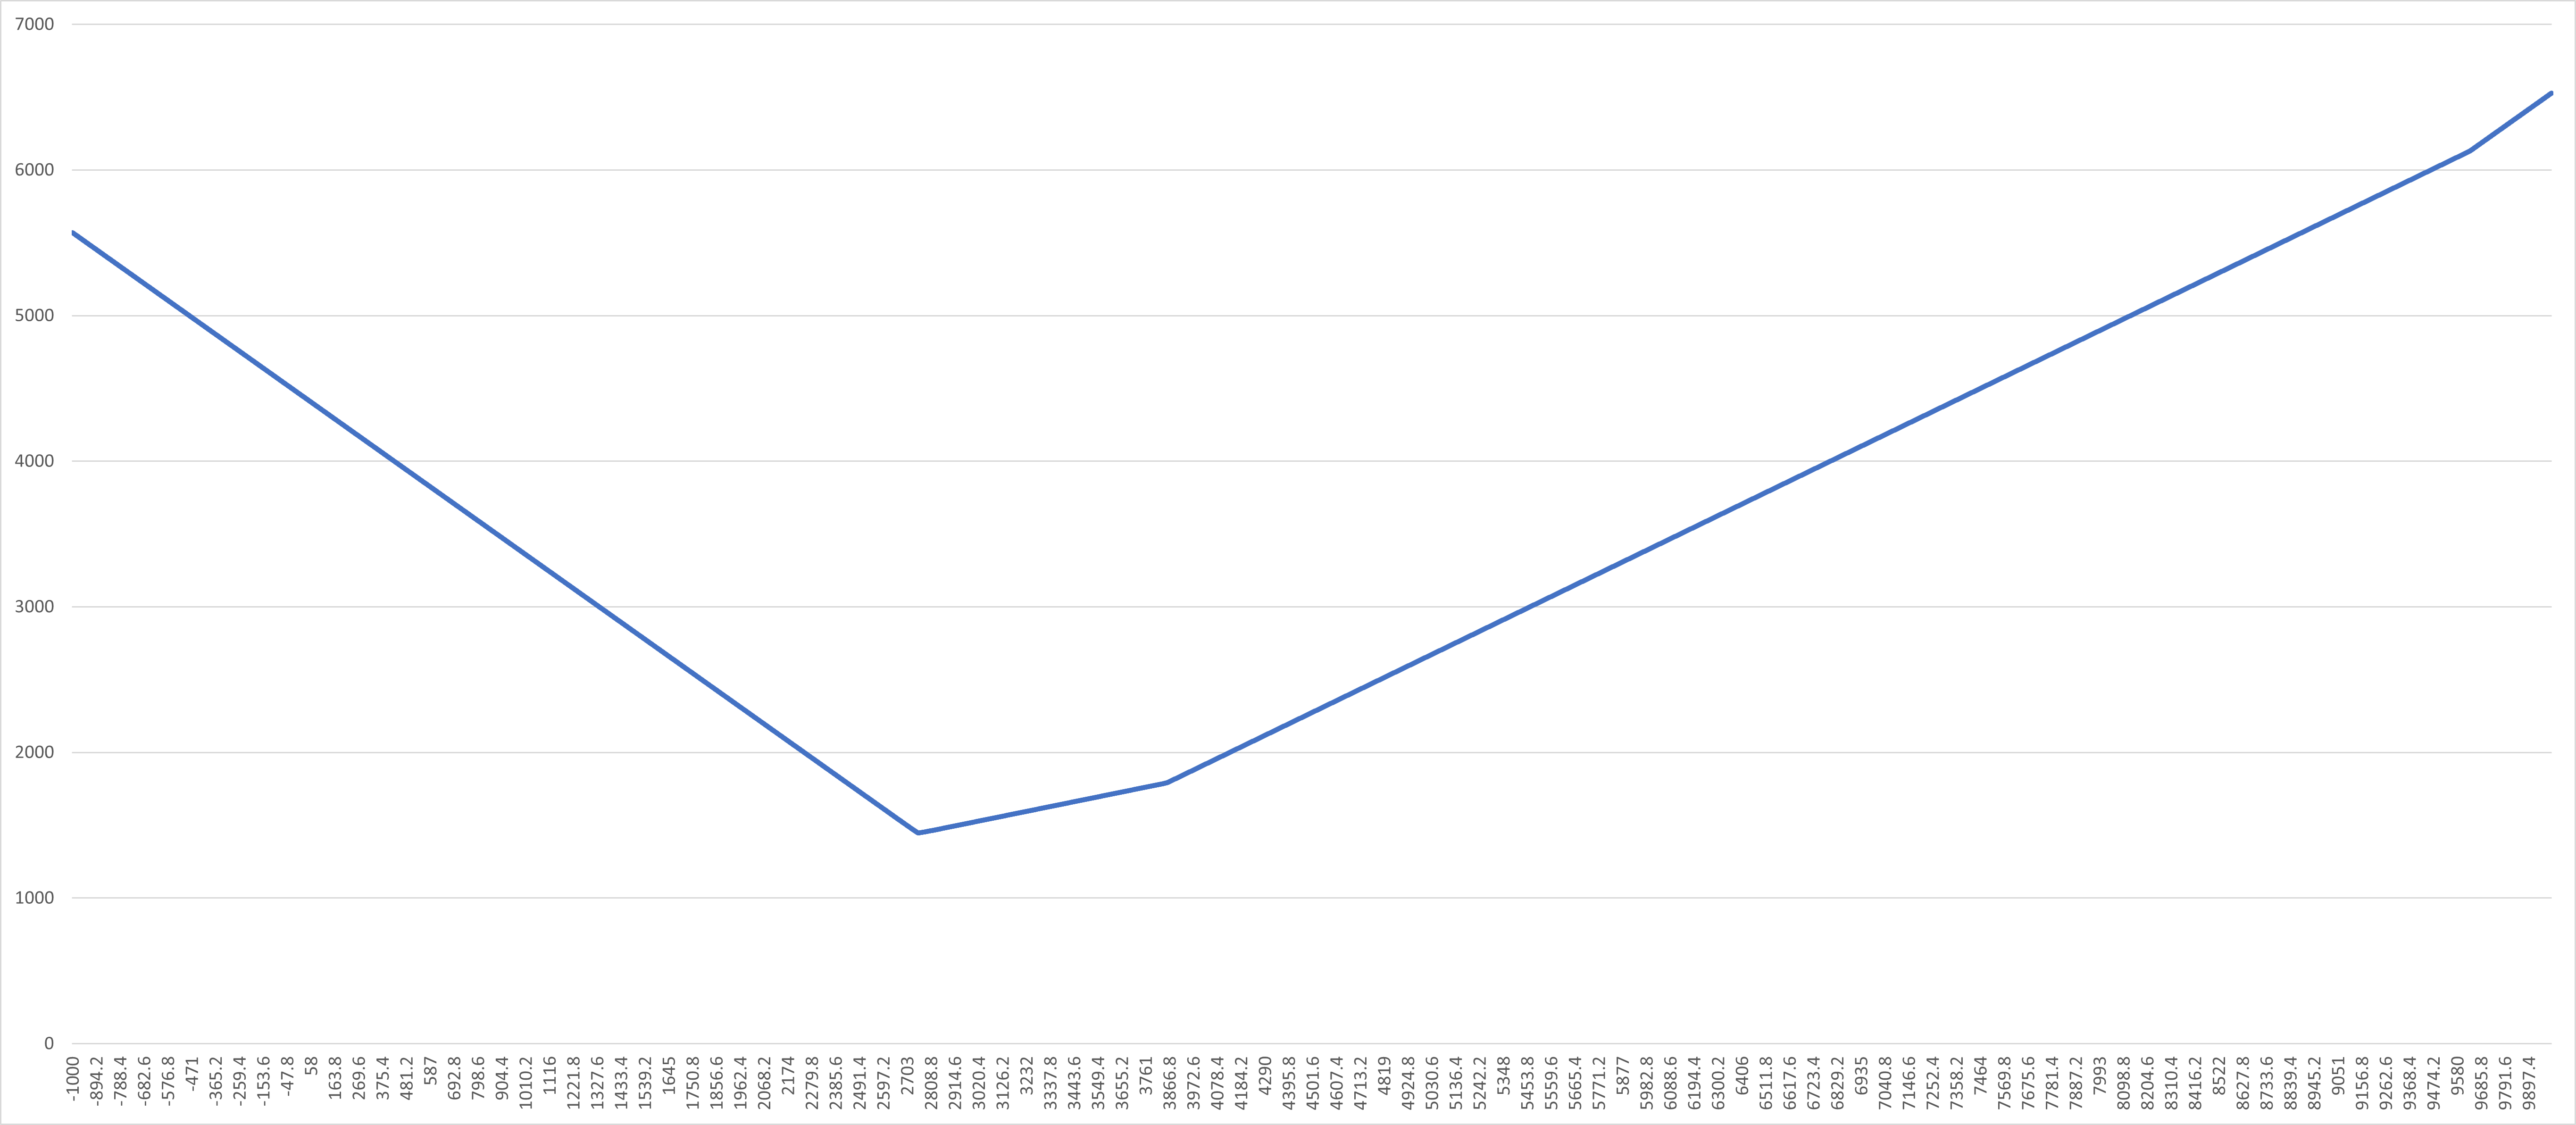
\includegraphics[scale=.33]{optstep1.png}\label{ex_optstep1}}\\
\subfigure[$g_f(h)$ for Example 2.]{
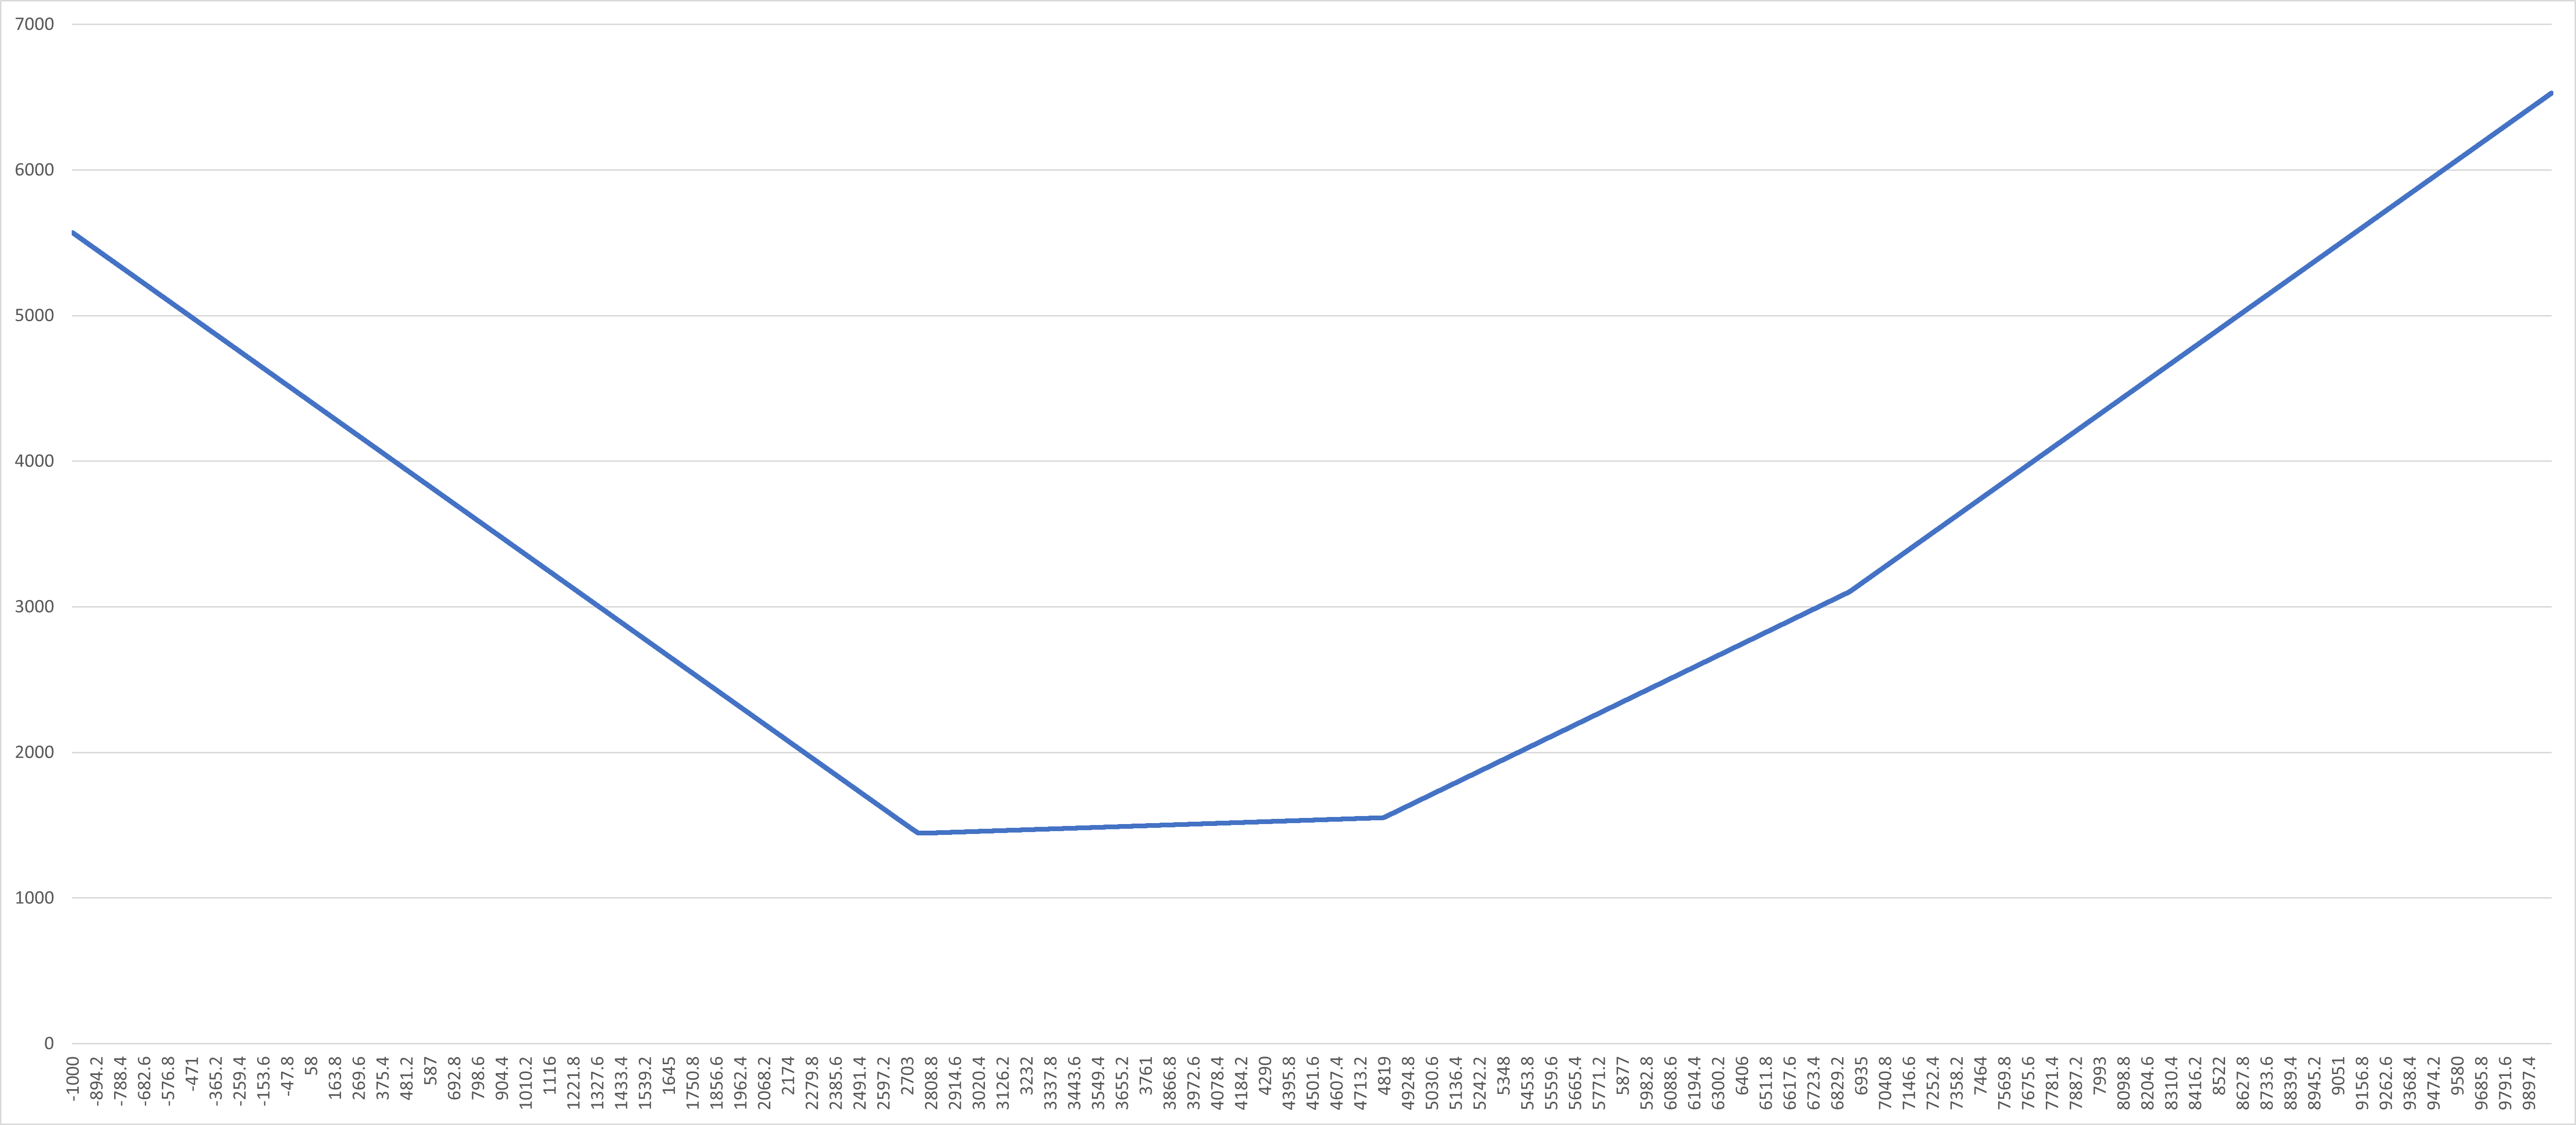
\includegraphics[scale=.33]{optstep2.png}\label{ex_optstep2}}\\
\subfigure[$g_f(h)$ for Example 3.]{
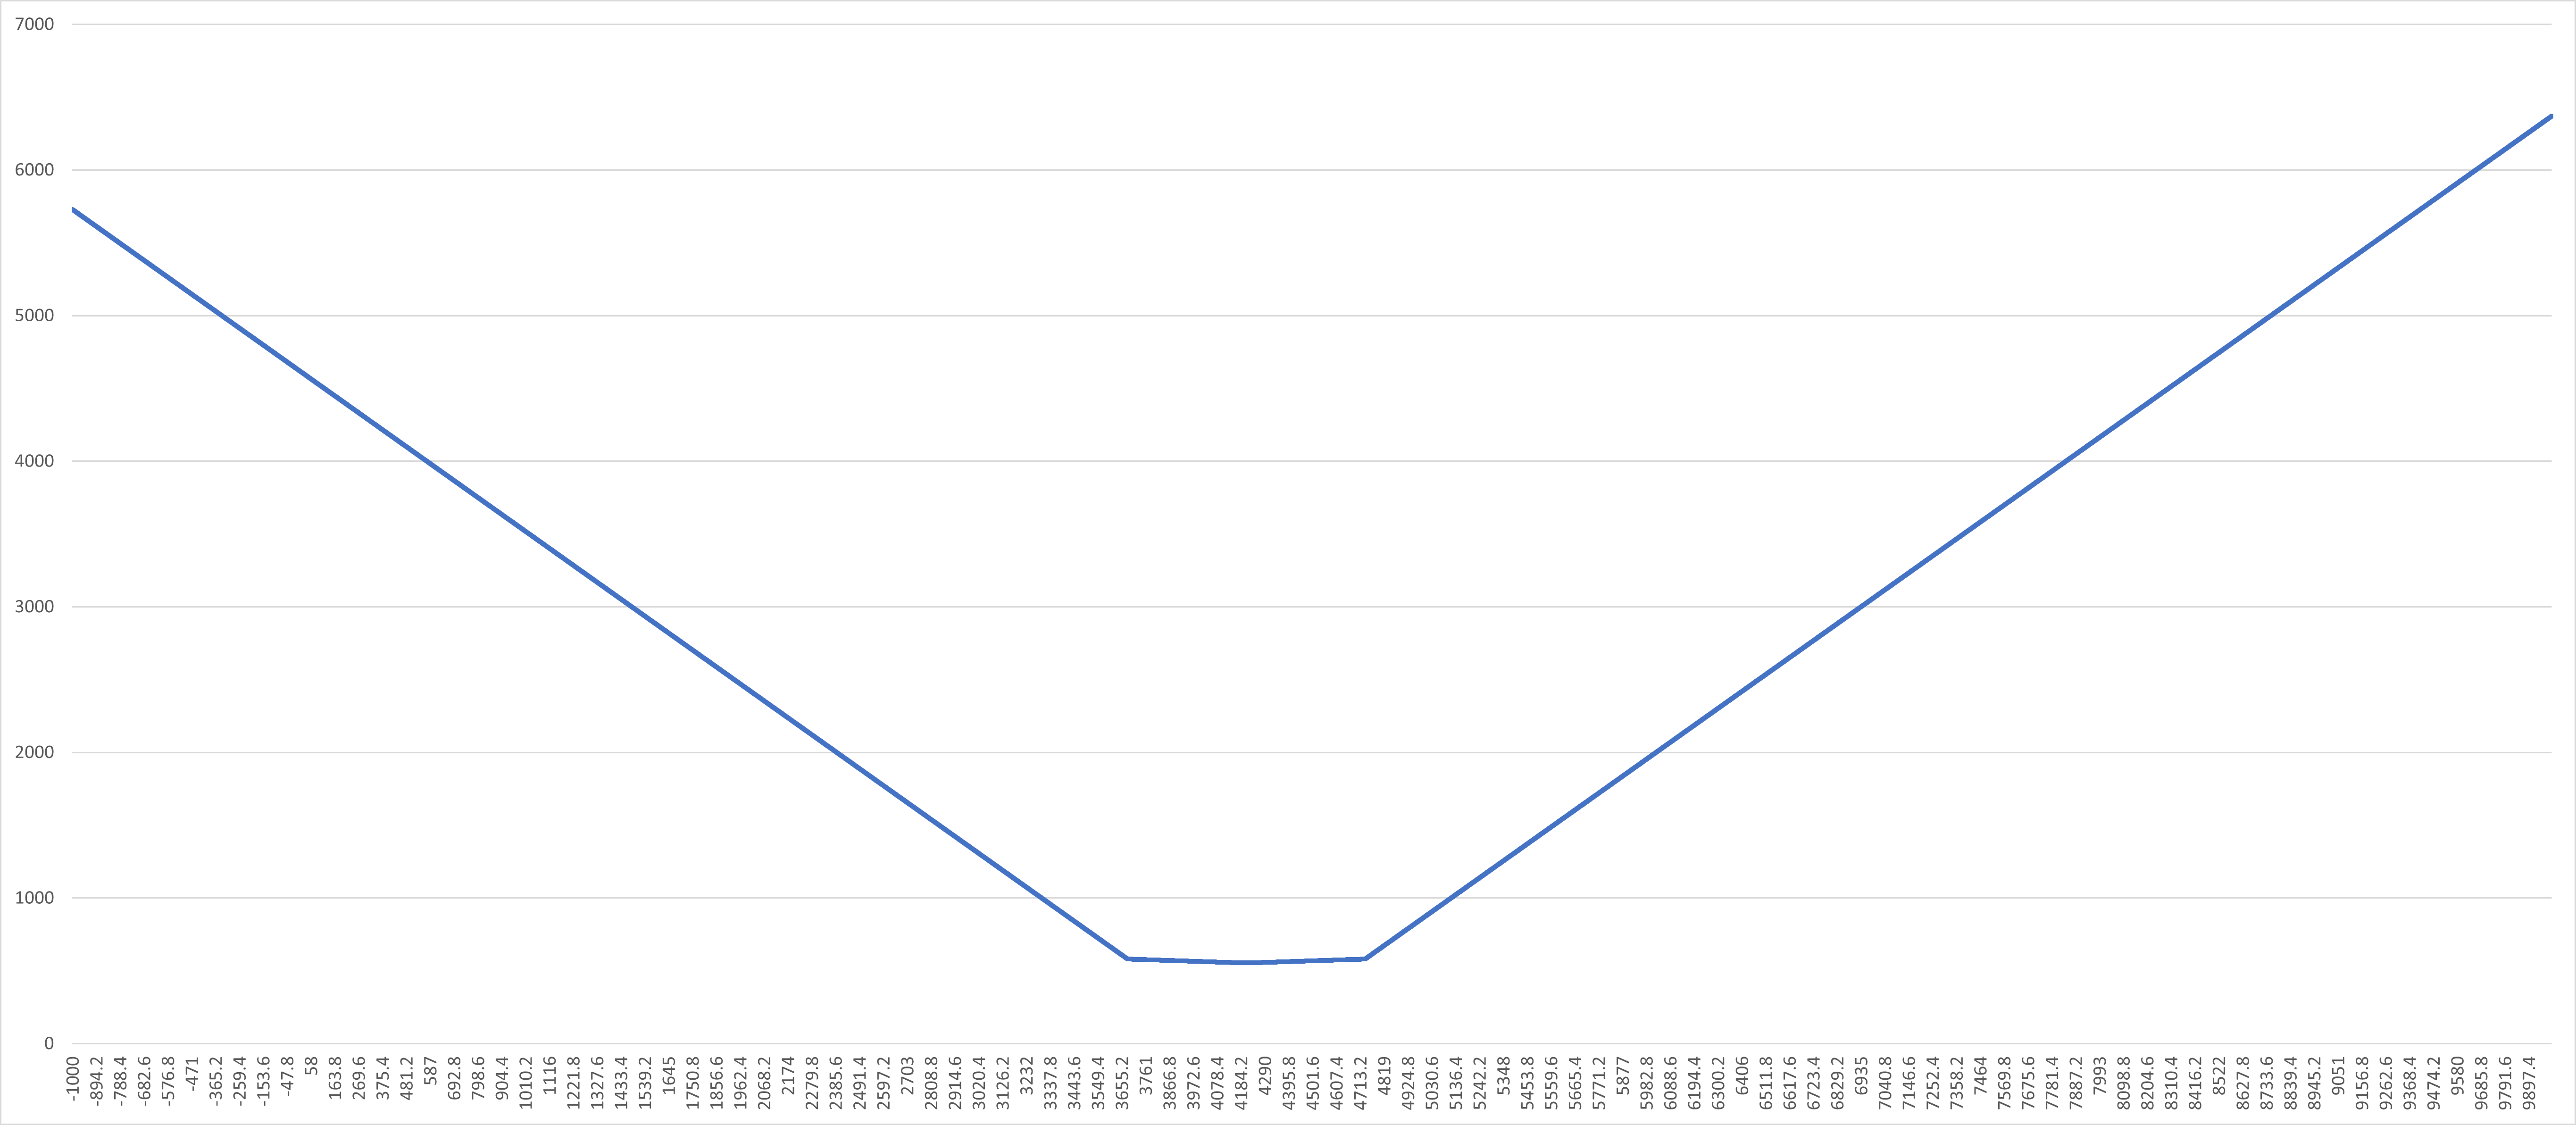
\includegraphics[scale=.33]{optstep3.png}\label{ex_optstep3}}
\caption{Examples for $g_f(h)$. }
\label{ex_optstep}
\end{figure}

\begin{figure}
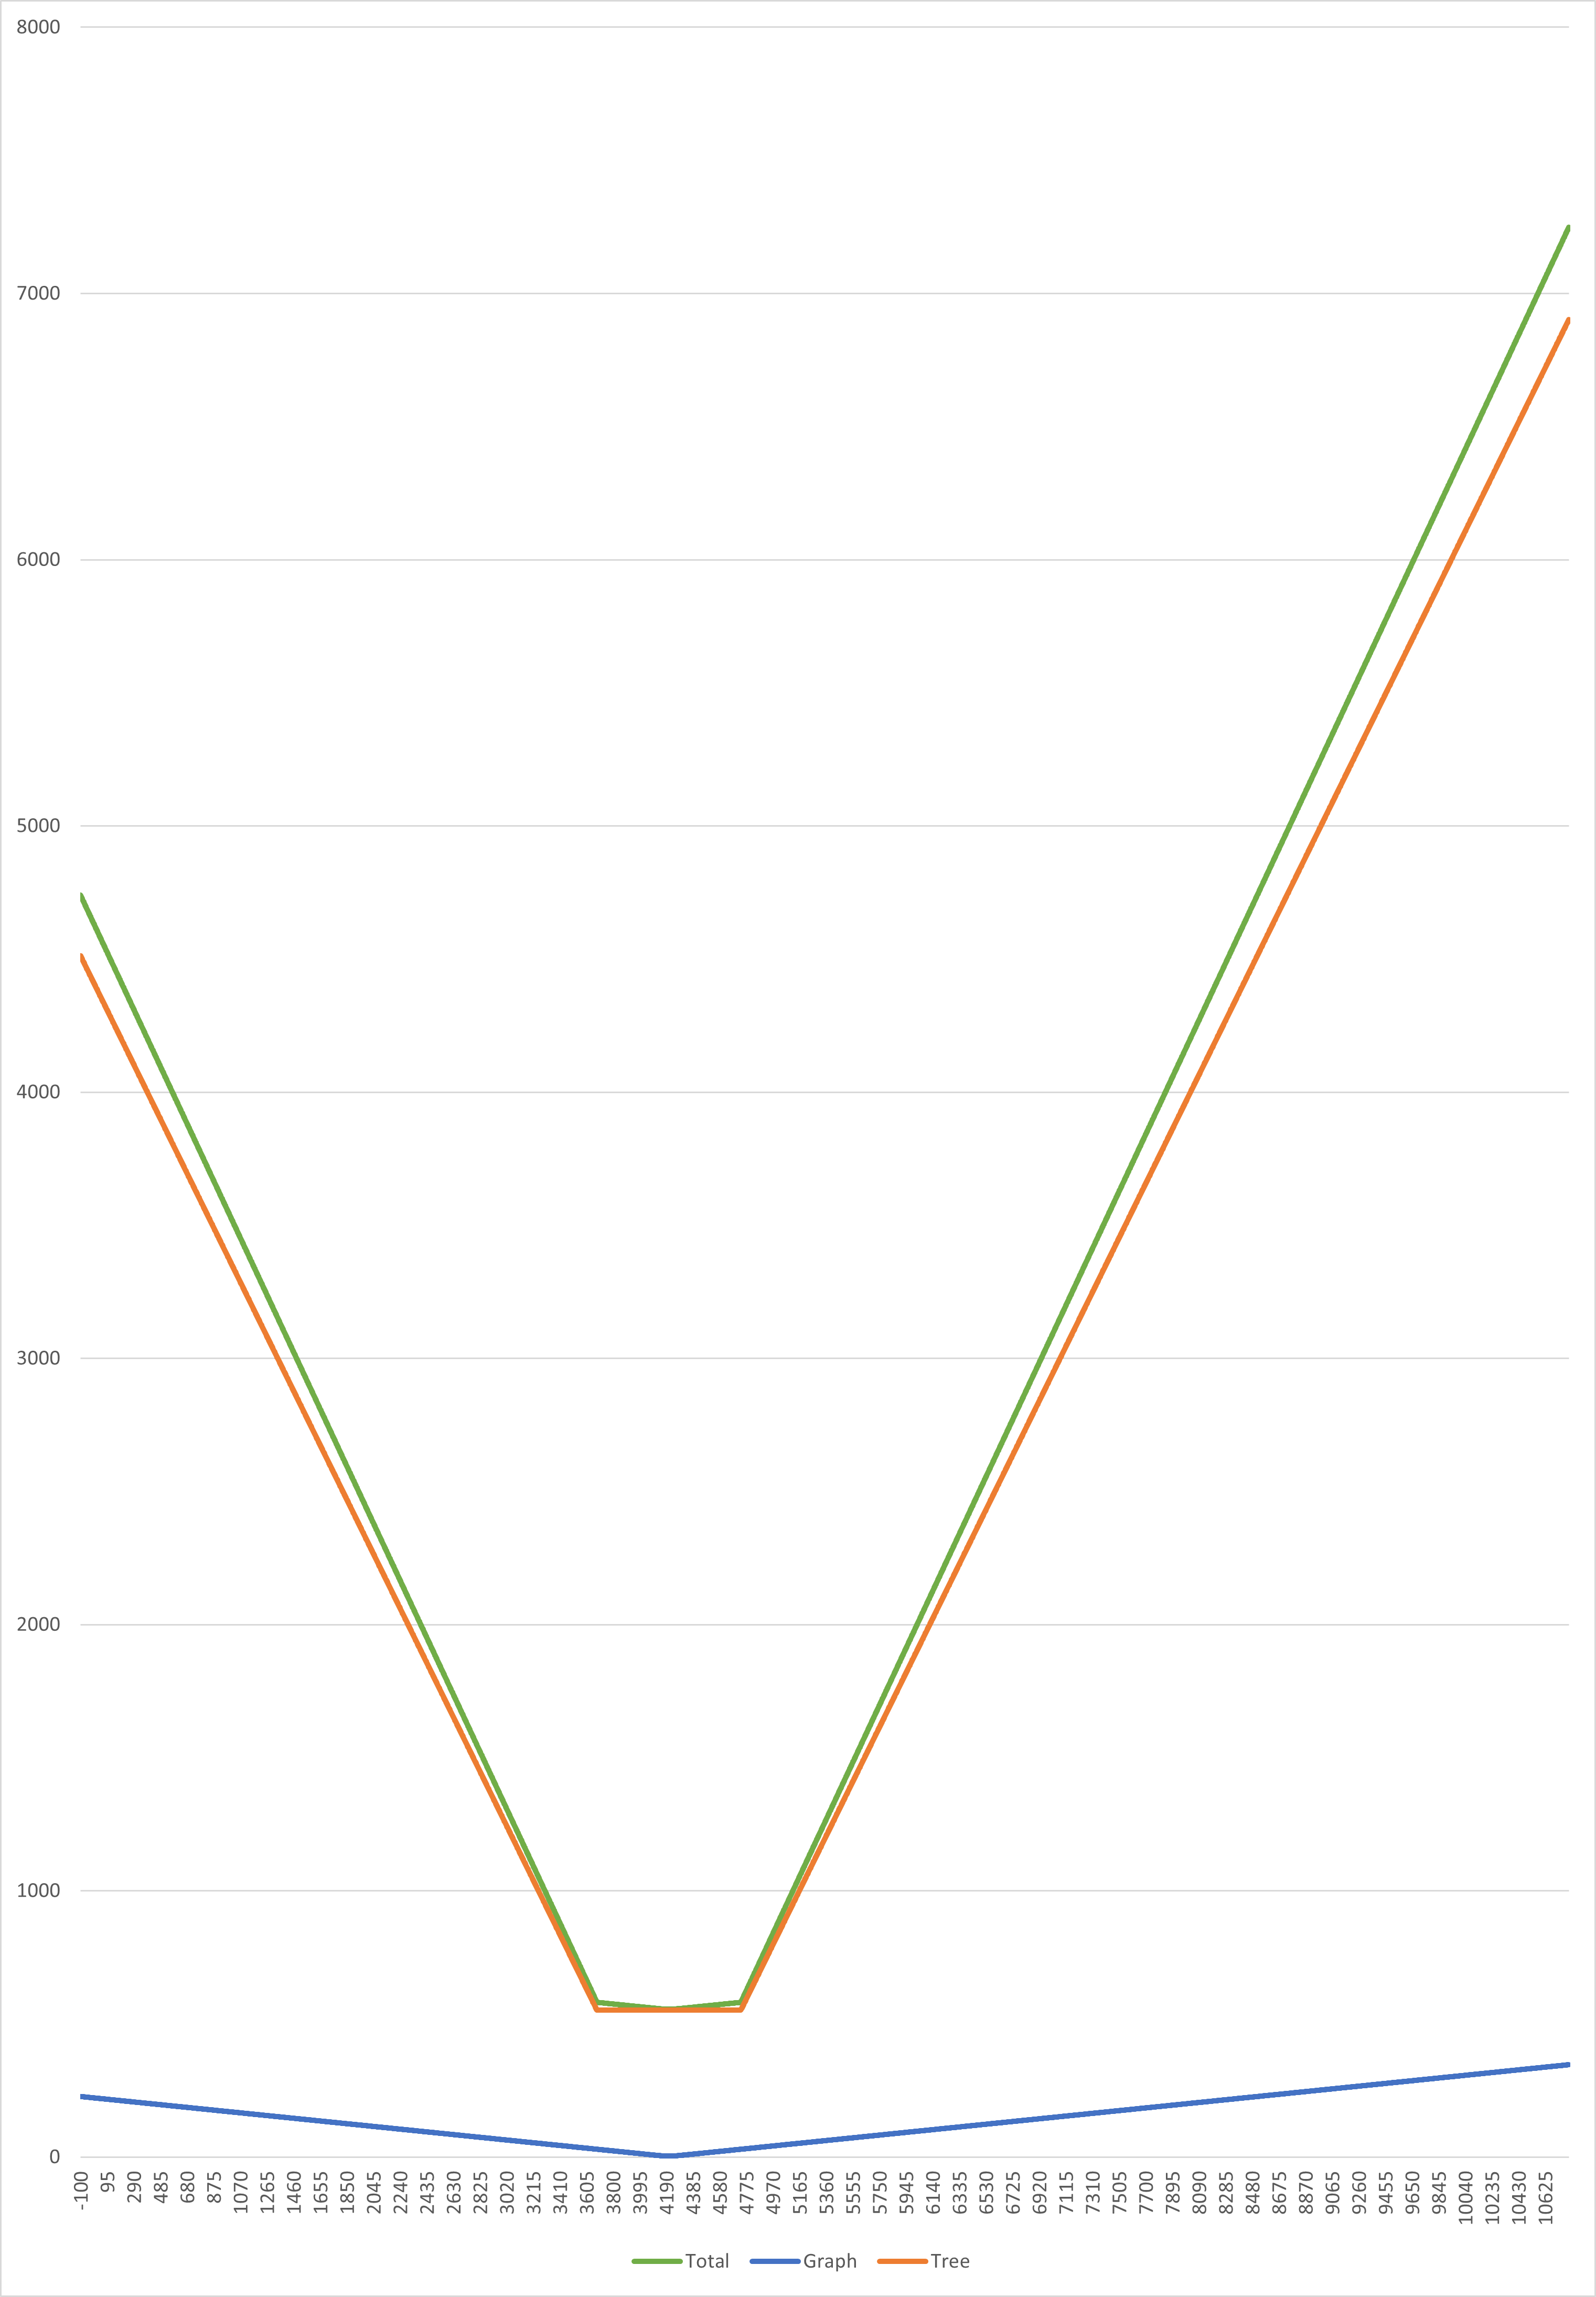
\includegraphics[scale=.62]{optstep3diff.png}
\caption{$g_f(h)$ for Example 3, split into $\phi=\phi_G+\phi_T$.}
\label{ex_optstep3diff}
\end{figure}
\begin{figure}
\subfigure[$g_f(h)$ for Example 3, refined.]{
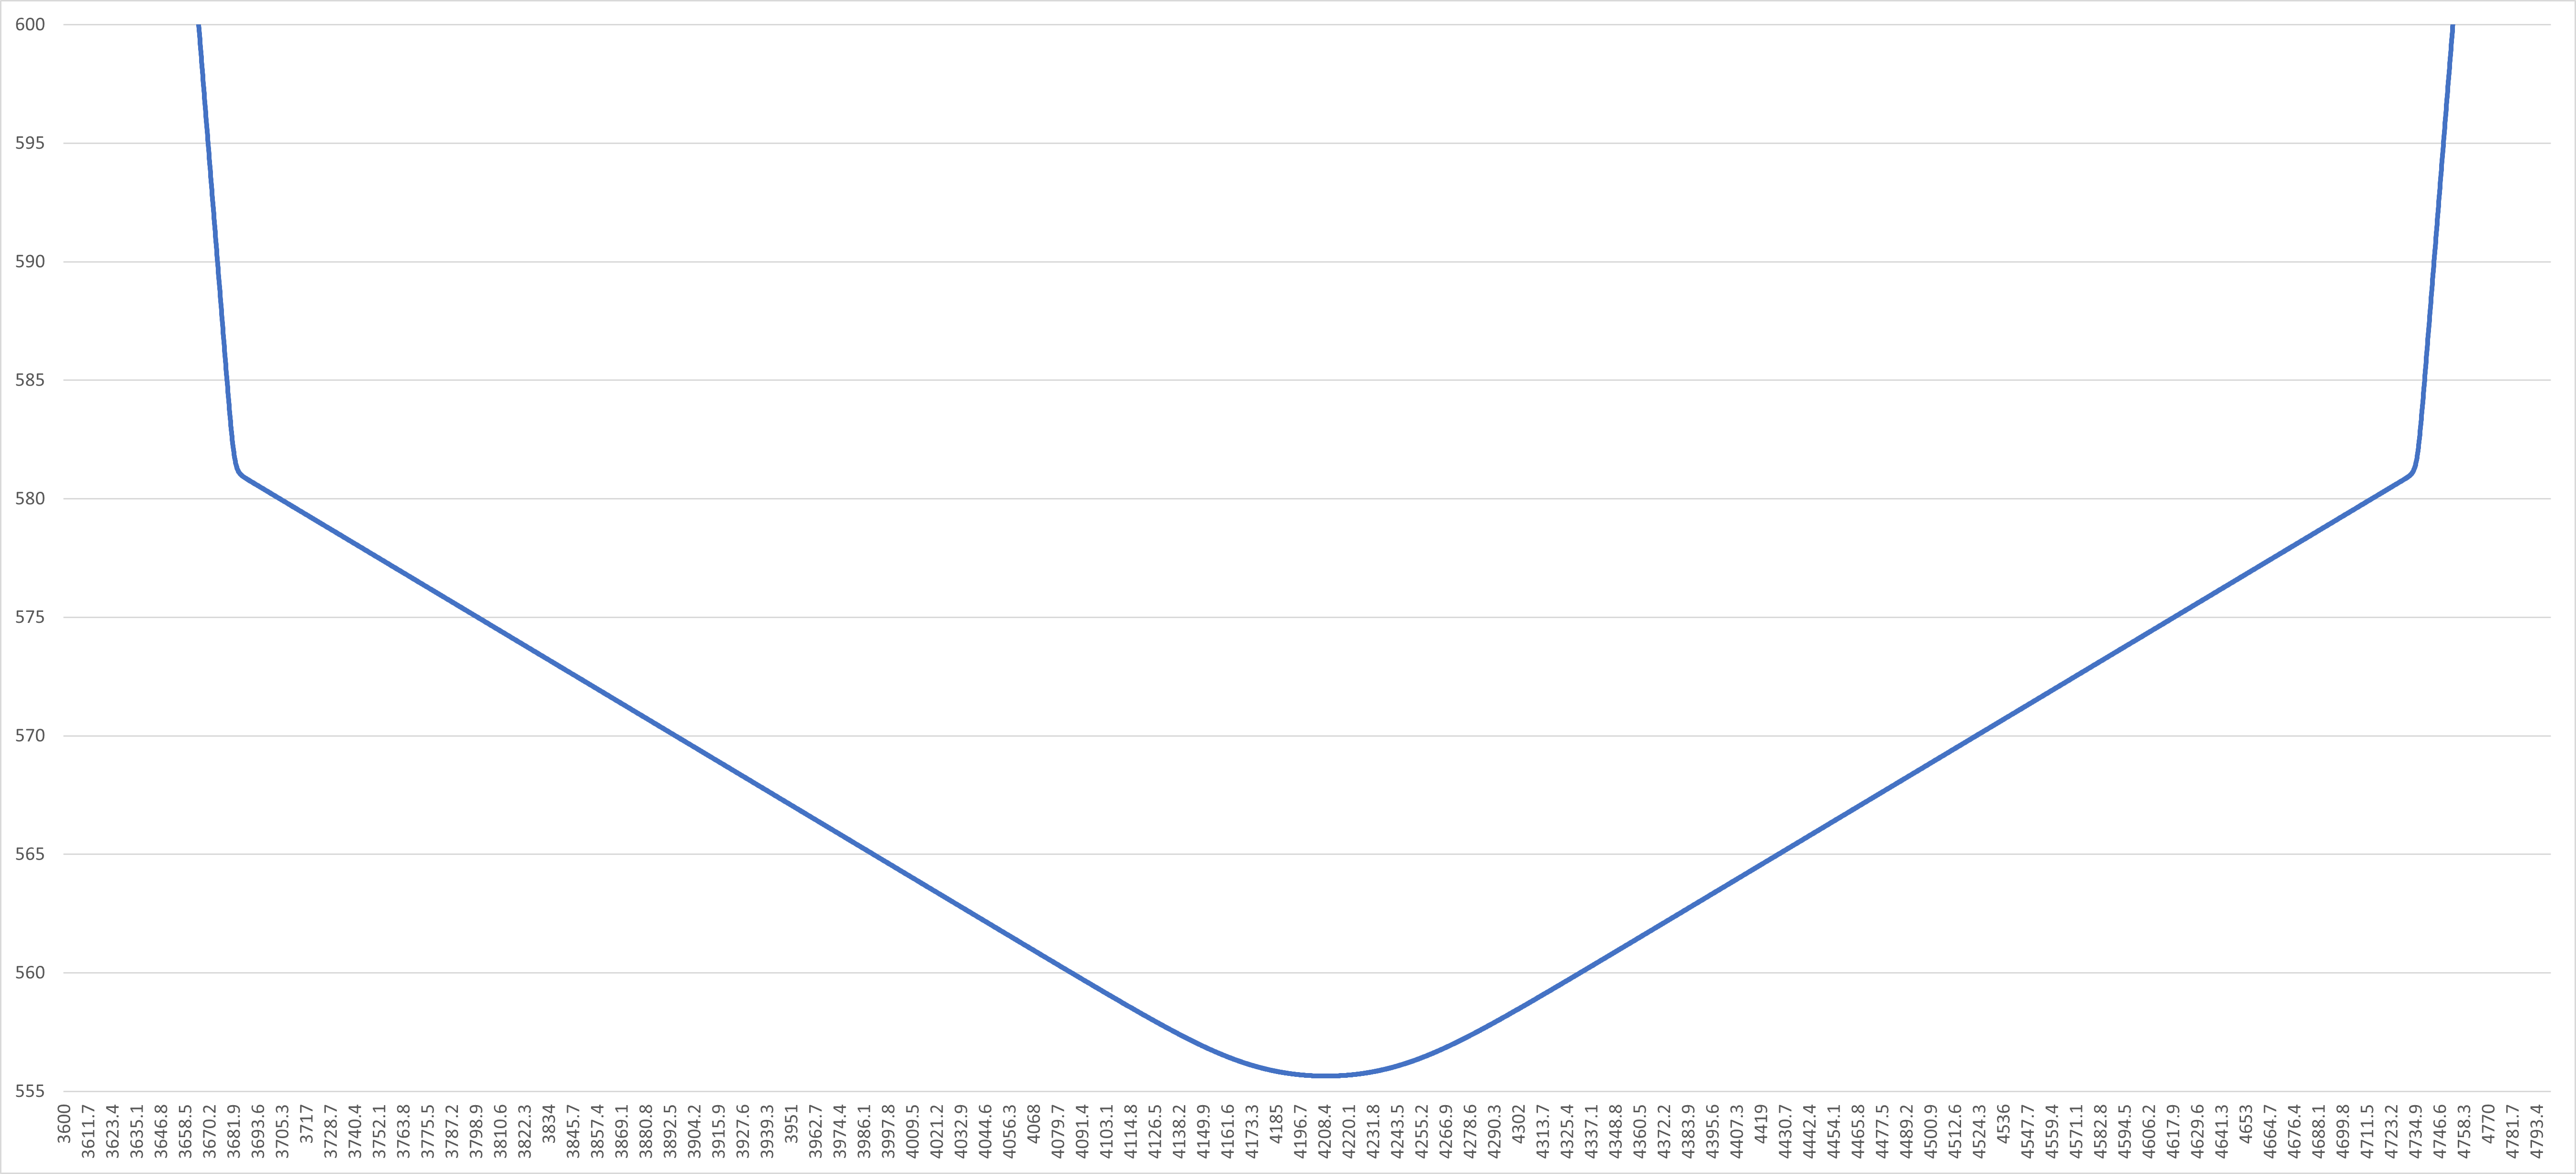
\includegraphics[scale=.33]{optstep3ref1.png}\label{ex_optstep3ref1}}\\
\subfigure[$g_f(h)$ for Example 3, further refined.]{
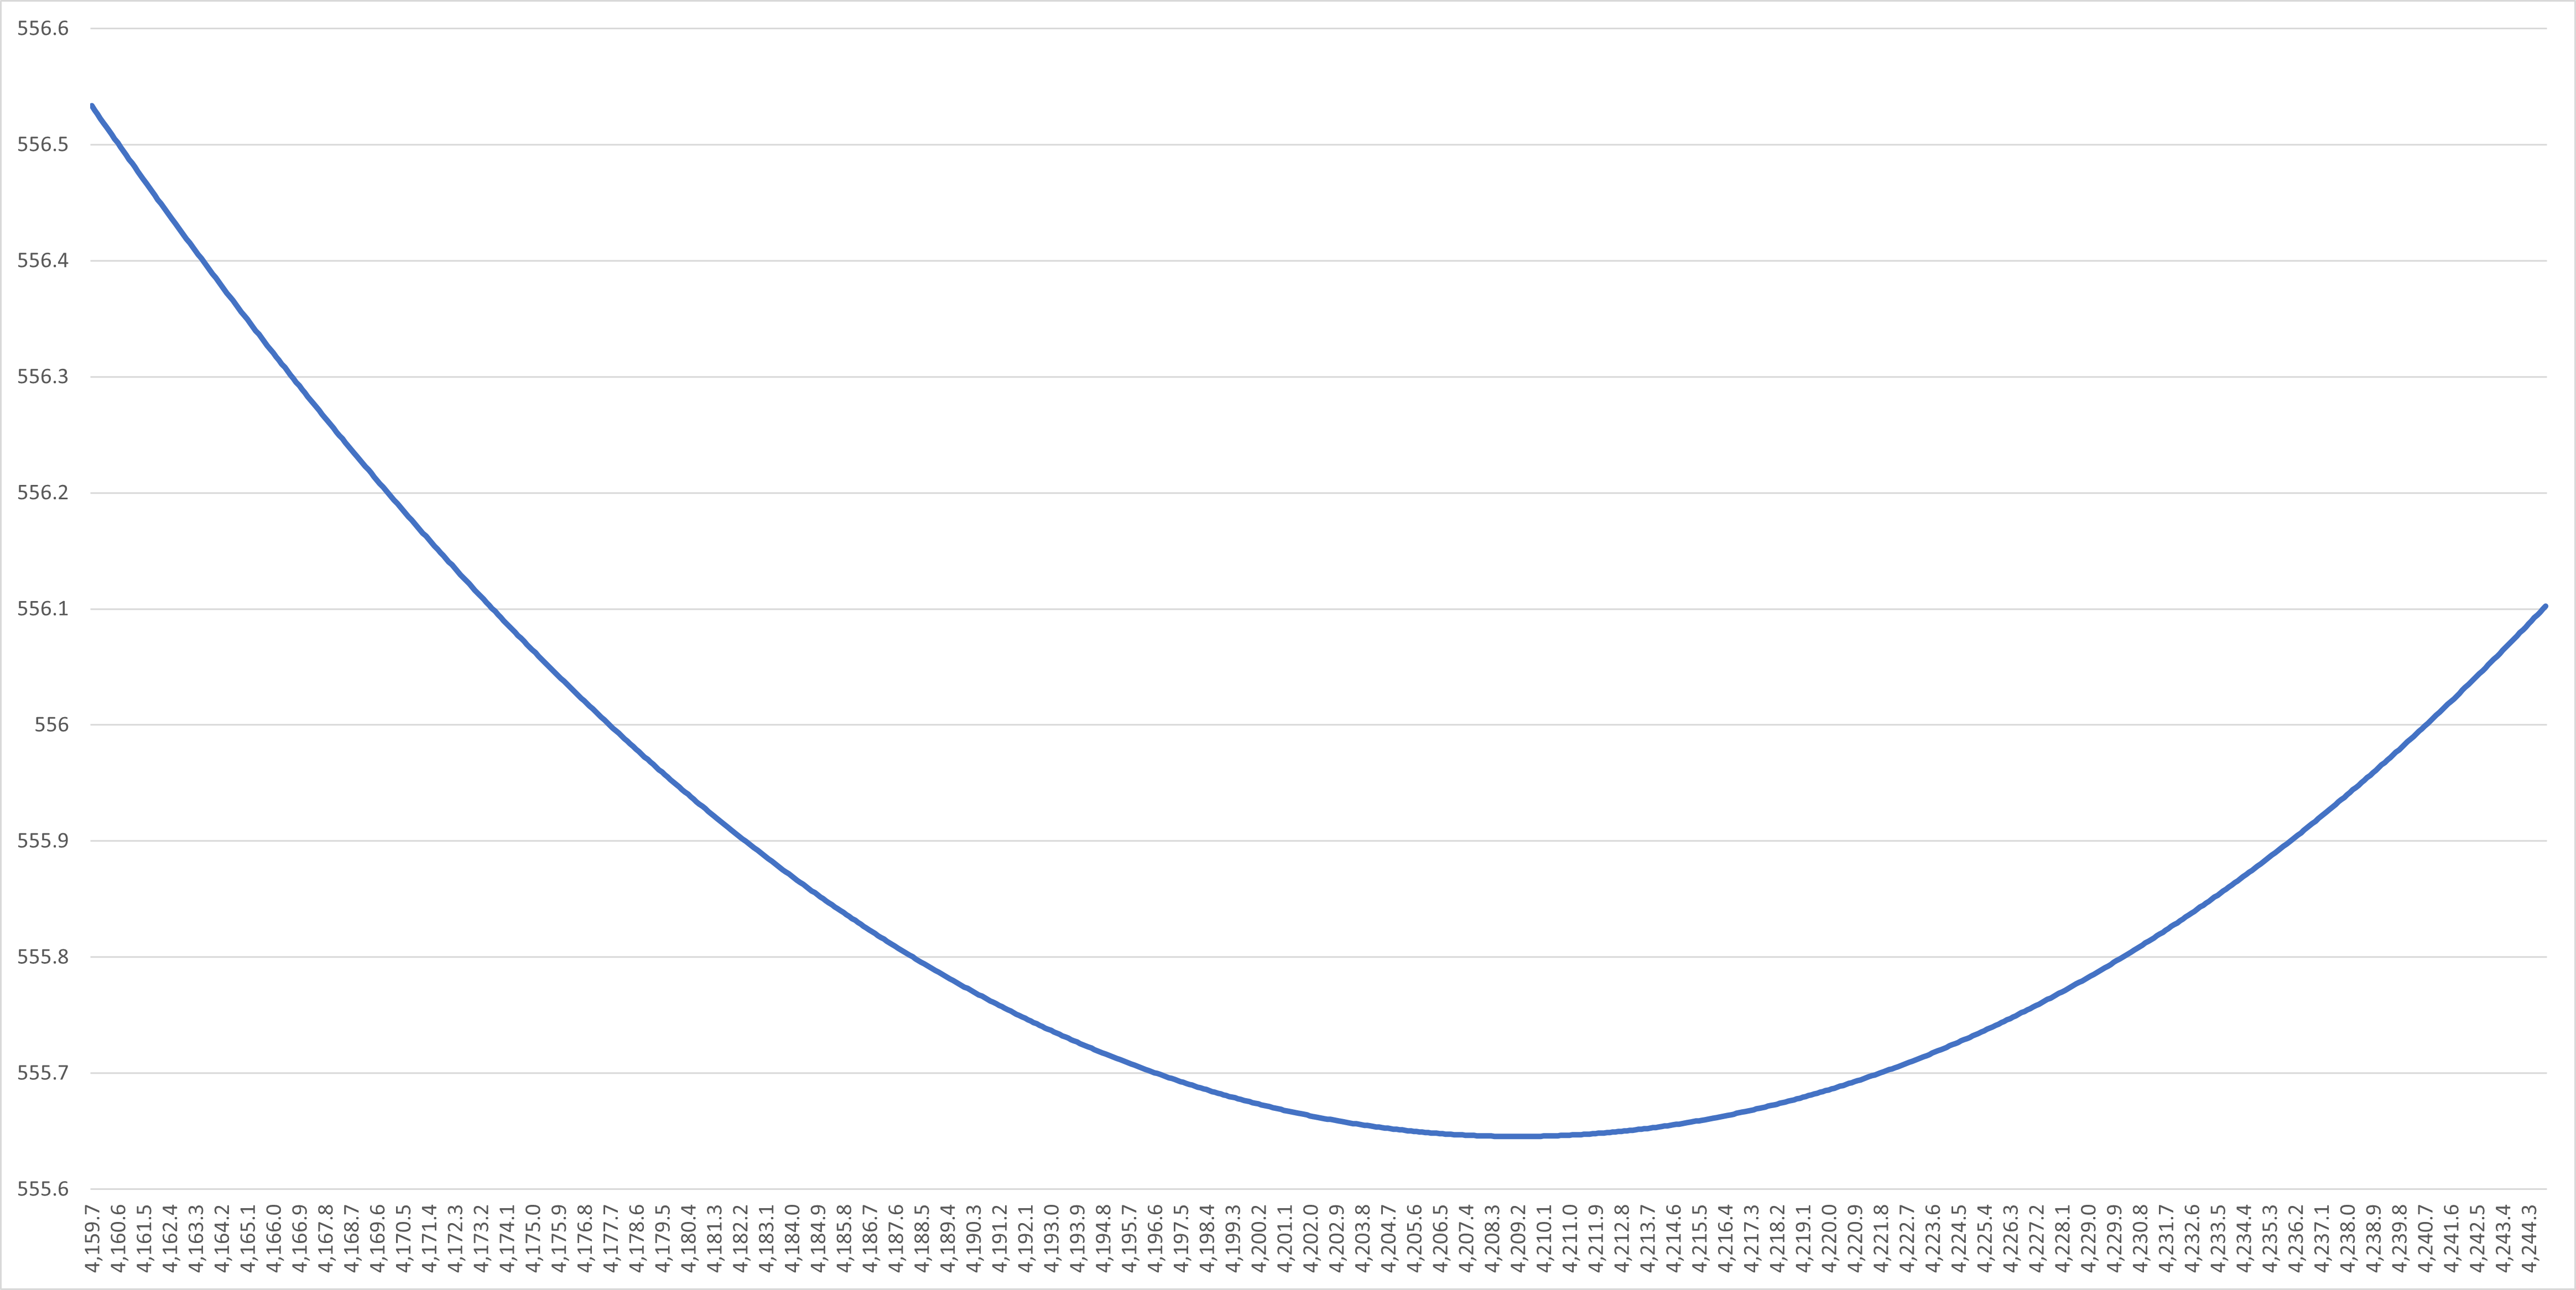
\includegraphics[scale=.38]{optstep3ref2.png}\label{ex_optstep3ref2}}
\caption{Refinements of $g_f(h)$ for Example 3, showing more detailed regions around the minimum.}
\label{ex_optstep3ref}
\end{figure}
\newpage
\subsection{Approach}
With $h^*$ denoting the (local) minimum, we assume $g_f(h)$ to be strictly monotonically decreasing for $h<h^*$ and strictly monotonically increasing for $h>h^*$, and thus, $h^*$ being the only local minimum of $g_f(h)$ and hence also the global minimum. With this assumption of strict monotonicity, we can search for the minimum with following scheme:
\begin{enumerate}
\item Search for $a_0$ and $b_0$ s.t. $a_0\leq h^*\leq b_0$
\item Start with $i=0$ and repeat:
\begin{enumerate}
\item Refine the interval from $[a_i,b_i]$ to $[a_{i+1},b_{i+1}]$ s.t. $a_{i+1}\geq a_i$, $b_{i+1}\leq b_i$, $b_{i+1}-a_{i+1}<b_i-a_i$ and $a_{i+1}\leq h^*\leq b_{i+1}$
\item Increment $i$
\item Terminate at some condition and output $\arg \min_{\{a_i,b_i\}}g_f$
\end{enumerate}
\end{enumerate}
The first step can be implemented by choosing an initial parameter $h_0$ and then, searching at higher parameters $h_1,h_2,...$ until a parameter $h_k$ is reached where $g_f(h_k)\geq g_f(h_{k-1})$. This would give us the information that $h^*$ lies in $[h_{k-2},h_k]$, if $k\geq 2$. If $k<2$, $h^*$ might be smaller than $h_0$. In this case, one could iterate a sequence with subsequently smaller parameters $h_{-1},h_{-2},...$ until a parameter $h_{-\overline{k}}$ is reached where $g_f(h_{-\overline{k}})\geq g_f(h_{-(\overline{k}-1)})$. Then, we could deduce that $h^*$ lies in $[h_{-\overline{k}},h_{-\overline{k}+2}]$. If $\overline{k}<2$, $h^*$ might be bigger than $h^0$. It can only be possible (based on our assumption of strict monotonicity) that $h^*$ is in $[h_{-1},h_1]$ if both directions instantly stop at $k=1=\overline{k}$.\\
A possible choice for those sequences is to define $h_{i}\coloneqq \gamma\cdot h_{i-1}$ and $h_{-i}\coloneqq \frac{1}{\gamma}\cdot h_{-(i-1)}$ for all $i\geq 1$ with $\gamma$ as growth factor.\\
This is also the sequence we use, where we set $\gamma=2$ and $h_0=1$. We will also postpone the search at $(0,h_{-2})$ and start with $h_{-2},h_{-1},h_0$, testing $g_f(h_0)<g_f(h_{-1})$, as our first idea is to accelerate the gradient-like descent and observe the impact - if the default parameter could be optimized by more than the precision of the minimum search with a decrease, we would still be able to decrease it downto $\frac{1}{4}$. This gives us algorithm \ref{alg_h_init} (note that algorithm \ref{alg_h_init} uses the indices $i$ in the expression $h_i$ dynamically). The results were generated using Algorithm \ref{alg_h_init}, whereas inspecting results from the enhanced version, Algorithm \ref{alg_h_init2}, are postponed for temporal reasons.
\begin{algorithm}
\caption{Calculation of Initial Search Interval for Line Search}\label{alg_h_init}
\begin{algorithmic}[1]
\Procedure{InitializeSearchInterval}{$f$}
\State $\gamma\gets 2$
\State $h_2\gets 1$
\State $h_1\gets h_2/\gamma$
\State $h_0\gets h_1/\gamma$
\State $(g_0,g_1,g_2)\gets (g_f(h_0),g_f(h_1),g_f(h_2))$
\While{$g_1>g_2$}
    \State $h_0\gets h_1$
    \State $h_1\gets h_2$
    \State $h_2\gets \gamma\cdot h_2$
    \State $g_0\gets g_1$
    \State $g_1\gets g_2$
    \State $g_2\gets g_f(h_2)$
\EndWhile
\State \Return $(h_0,h_2)$
\EndProcedure
\end{algorithmic}
\end{algorithm}
\begin{algorithm}
\caption{Enhanced Version of Algorithm \ref{alg_h_init}}\label{alg_h_init2}
\begin{algorithmic}[1]
\Procedure{InitializeSearchInterval}{$f$, $\gamma$, $h_0$}
\State $h_1\gets \gamma\cdot h_0$
\State $(g_0, g_1)\gets (g_f(h_0),g_f(h_1))$
\State $i\gets 1$
\While{$g_{i-1}>g_i$}
    \State $i\gets i+1$
    \State $h_i\gets \gamma\cdot h_{i-1}$
    \State $g_i\gets g_f(h_i)$
\EndWhile
\If{$i=1$}
    \State $h_{-1}\gets h_0/\gamma$
    \State $g_{-1}\gets g_f(h_{-1})$
    \State $j\gets -1$
    \While{$g_j<g_{j+1}$}
        \State $j\gets j-1$
        \State $h_j\gets h_{j+1}/\gamma$
        \State $g_j\gets g_f(h_j)$
    \EndWhile
    \State \Return $(h_j,h_{j+2})$
\Else
    \State \Return $(h_{i-2},h_i)$
\EndIf
\EndProcedure
\end{algorithmic}
\end{algorithm}


The interval refinement can be done via Ternary Search: Select two points $l_i,r_i$ inside $[a_i,b_i]$ (``Ternary Search'' uses $l_i=a_i+\frac{1}{3}\cdot (b_i-a_i)$ and $r_i=a_i+\frac{2}{3}\cdot (b_i-a_i)$) and compare $g_f(l_i)$ with $g_f(r_i)$. As can be seen in Figure \ref{ex_ls5}, we now can deduce from the four points we have that $h^*$ is either in one or two out of our three intervals. In all cases, we can be sure that at least one interval does not contain the minimum, based on our assumptions, namely $[a_i,l_i)$, if $g_f(l_i)\geq g_f(r_i)$, or $(r_i,b_i]$, if $g_f(l_i)\leq g_f(r_i)$. This interval is discarded.\\
Since the function evaluation is \textit{very} expensive relatively to the rest of the iteration, we use the Golden-Section Search, which works just like the Ternary Search, but has less function evaluations and a better interval shrinking factor. \\
Before elaborating further, we will shortly discuss the termination condition.
Usually, one is interested in having the function \textit{parameter}, $h$ in our case, as precisely as possible, so a fitting termination condition would be that $\vert a_i-b_i\vert$ is below some threshold. This is not the case for us, as we are only interested in a function \textit{value} that is as small as possible, so a termination condition concerning the precision of the function value would be more fitting. This is a bit more tricky, as we don't have a precision estimate, since, for the parameter with $h^*\in[a_i,b_i]$, we can only use $g_f(h^*)\leq \min\{g_f(a_i),g_f(b_i)\}$. With the current assumptions, it would be possible for $h^*$ to be arbitrarily small. But it is \textit{very likely} that $g_f(h)$ is also convex, so linear extrapolation at $[a_i\leftrightarrow l_i\rightarrow]$ for $(l_i,b_i]$ or at $[\leftarrow r_i\leftrightarrow b_i]$ for $[a_i,r_i)$ could be used to estimate the maximum error of the function \textit{value} of $g_f(h^*)$, based on the new assumption.\\
This will be implemented in the future, but for now, we will use $\vert g_f(l_i)-g_f(r_i)\vert<\rho$ as termination condition for some precision parameter $\rho$. Note that this is bad design, but an easy condition to start with, as it is a necessary, but not sufficient indicator that our approximation is precise. The results shown later use this ``bad'' termination condition.
\begin{figure}
\subfigure[3 Points, conclusive]{
\begin{tikzpicture}
  \begin{axis}[
      domain=-3:3,
      ticks=none,
      %axis x line=bottom,
      %axis y line=left,
      xlabel = $h$,
      ylabel = $g_f(h)$,
      width = 0.5 \textwidth,
      height = 3.3cm,
    ]
    \addplot[Green, no marks, restrict x to domain=-1:1] {0.2*x^2+1};
    \addplot[blue, no marks, restrict x to domain=1:2] {0.2*x^2+1};
    \addplot[blue!20, no marks, restrict x to domain=-3:-1] {0.2*x^2+1};
    \addplot[blue!20, no marks, restrict x to domain=2:3] {0.2*x^2+1};
    \addplot[only marks, Green, samples at={-1,1,2}]{0.2*x^2+1};
  \end{axis}
\end{tikzpicture}\label{ex_ls1}}%
\subfigure[3 Points, inconclusive]{
\begin{tikzpicture}
  \begin{axis}[
      domain=-1.2:1.2,
      ticks=none,
      %axis x line=bottom,
      %axis y line=left,
      xlabel = $h$,
      %ylabel = $g_f(h)$,
      width = 0.5 \textwidth,
      height = 3.3cm,
    ]
    \addplot[blue!20, no marks, restrict x to domain=-1.2:-1] {0.15*x^4+0.25*x^3+0.85*x^2-0.25*x};
    \addplot[cyan!20, no marks, restrict x to domain=-1.2:-1] {0.15*x^4-0.25*x^3+0.85*x^2+0.25*x};
    \addplot[blue, no marks, restrict x to domain=-1:1] {0.15*x^4+0.25*x^3+0.85*x^2-0.25*x};
    \addplot[cyan, no marks, restrict x to domain=-1:1] {0.15*x^4-0.25*x^3+0.85*x^2+0.25*x};
    \addplot[blue!20, no marks, restrict x to domain=1:1.2] {0.15*x^4+0.25*x^3+0.85*x^2-0.25*x};
    \addplot[cyan!20, no marks, restrict x to domain=1:1.2] {0.15*x^4-0.25*x^3+0.85*x^2+0.25*x};
    \addplot[only marks, red, samples at={-1,0,1}]{0.15*x^4+0.25*x^3+0.85*x^2-0.25*x};
  \end{axis}
\end{tikzpicture}\label{ex_ls2}}\\
\subfigure[4 Points, minimum at border]{
\begin{tikzpicture}
  \begin{axis}[
      domain=-3:3,
      ticks=none,
      %axis x line=bottom,
      %axis y line=left,
      xlabel = $h$,
      ylabel = $g_f(h)$,
      width = 0.5 \textwidth,
      height = 3.3cm,
    ]
    \addplot[blue, no marks, restrict x to domain=-1:2.8] {0.2*x^2+1};
    \addplot[blue!20, no marks, restrict x to domain=-3:-1] {0.2*x^2+1};
    \addplot[blue!20, no marks, restrict x to domain=2.7:3] {0.2*x^2+1};
    \addplot[only marks, Green, samples at={-1,1,1.7,2.7}]{0.2*x^2+1};
  \end{axis}
\end{tikzpicture}\label{ex_ls3}}%
\subfigure[4 Points, minimum at center]{
\begin{tikzpicture}
  \begin{axis}[
      domain=-3:3,
      ticks=none,
      %axis x line=bottom,
      %axis y line=left,
      xlabel = $h$,
      %ylabel = $g_f(h)$,
      width = 0.5 \textwidth,
      height = 3.3cm,
    ]
    \addplot[blue, no marks, restrict x to domain=-2:2] {0.2*x^2+1};
    \addplot[blue!20, no marks, restrict x to domain=-3:-2] {0.2*x^2+1};
    \addplot[blue!20, no marks, restrict x to domain=2:3] {0.2*x^2+1};
    \addplot[only marks, Green, samples at={-2,-1,1,2}]{0.2*x^2+1};
  \end{axis}
\end{tikzpicture}\label{ex_ls4}}\\
\subfigure[Conclusion from strict monotonicity assumption]{
\begin{tikzpicture}
  \begin{axis}[
      domain=-3:3,
      ticks=none,
      %axis x line=bottom,
      %axis y line=left,
      xlabel = $h$,
      ylabel = $g_f(h)$,
      width = 0.5 \textwidth,
      height = 3.3cm,
    ]
    \addplot[blue!20, no marks, restrict x to domain=-3:-2.8] {0.2*x^2+1};
    \addplot[blue!20, no marks, restrict x to domain=2.8:3] {0.2*x^2+1};
    \addplot[blue, no marks, restrict x to domain=-2.8:-1] {0.2*x^2+1};
    \addplot[blue, no marks, restrict x to domain=1:2.8] {0.2*x^2+1};
    \addplot[Green, no marks, restrict x to domain=-1:1] {0.2*x^2+1};
    \addplot[only marks, blue, samples at={-2.8,-2,-1,1,2,2.8}]{0.2*x^2+1};
    \addplot[mark=*,Green] coordinates {(0,1)};
  \end{axis}
\end{tikzpicture}\vspace{0.2cm}
\begin{tikzpicture}
  \begin{axis}[
      domain=-3:3,
      ticks=none,
      %axis x line=bottom,
      %axis y line=left,
      xlabel = $h$,
      %ylabel = $g_f(h)$,
      width = 0.5 \textwidth,
      height = 3.3cm,
    ]
    \addplot[blue!20, no marks, restrict x to domain=-3:-2.8] {0.2*x^2+1};
    \addplot[blue!20, no marks, restrict x to domain=2.8:3] {0.2*x^2+1};
    \addplot[blue, no marks, restrict x to domain=-2.8:-1] {0.2*x^2+1};
    \addplot[blue, no marks, restrict x to domain=1:2.8] {0.2*x^2+1};
    \addplot[Green, no marks, restrict x to domain=-1:1] {0.2*x^2+1};
    \addplot[only marks, blue, samples at={-2.8,-2,2,2.8}]{0.2*x^2+1};
    \addplot[only marks, Green, samples at={-1,1}]{0.2*x^2+1};
  \end{axis}
\end{tikzpicture}
\label{ex_ls5}}
\label{ex_linesearch}
\caption{Visualization of the cases during line search. The function is assumed to have a local minimum between the two border points, for which the function strictly monotonically decreases before and strictly monotonically increases after this minimum (strict monotonicity assumption).}
\end{figure}

\subsection{Golden-Section Search}
The Golden-Section Search uses intermediate points $l_i=b_i-\frac{b_i-a_i}{\varphi}$ and $r_i=a_i+\frac{b_i-a_i}{\varphi}$, where $\varphi\coloneqq\frac{1+\sqrt{5}}{2}$ is called ``golden section''. Directly matching the expression to the quadratic formula shows the fact $\varphi^2-\varphi-1=0$, from which we can also derive $\varphi(\varphi-1)=1$, $\varphi^2=\varphi+1$ and $\frac{1}{\varphi}=\varphi-1$.\\
When we sort out the interval $(r_i,b_i]$, the new interval would be $[a_{i+1},b_{i+1}]$ with $a_{i+1}=a_i$, $b_{i+1}=r_i$, size $b_{i+1}-a_{i+1}=\frac{b_i-a_i}{\varphi}$, $l_{i+1}=b_{i+1}-\frac{b_{i+1}-a_{i+1}}{\varphi}$ and $r_{i+1}=a_{i+1}+\frac{b_{i+1}-a_{i+1}}{\varphi}$. We can now prove that $r_{i+1}=l_i$:
\begin{align*}
r_{i+1}&=a_{i+1}+\frac{b_{i+1}-a_{i+1}}{\varphi}\\
&=a_i+\frac{b_i-a_i}{\varphi^2}\\
&=a_i+(b_i-a_i)\cdot (\varphi-1)^2\\
&=a_i+(b_i-a_i)\cdot (\varphi^2-2\varphi+1 )\\
&=a_i+(b_i-a_i)\cdot (2-\varphi)\\
&=(b_i-a_i)+a_i+(b_i-a_i)\cdot (1-\varphi)\\
&=b_i-(b_i-a_i)\cdot (\varphi-1)\\
&=b_i-\frac{b_i-a_i}{\varphi}\\
&=l_i~.~\square
\end{align*}
This proof can be done symmetrically for $l_{i+1}=r_i$ for the other case of sorting out $[a_i,l_i)$. This fact implies that we only need to evaluate the function at one intermediate point, while the other intermediate point is already evaluated, as it is conserved from iteration $i$.
\subsection{Possible Enhancements}
As already mentioned, there are many possible enhancements or alternatives at this stage, but they are postponed for temporal reasons, for example:
\begin{itemize}
\item Extend initial phase to both directions (see Algorithm \ref{alg_h_init2})
\item Optimized growth factor in initial phase
\item Extrapolation-based precision estimate for $\frac{\min\{g_f(a_i),g_f(b_i)\}}{g_f(h^*)}$ and better extrapolation techniques as described earlier
\item Implementation of $g_f'$, enabling Binary Search or a better extrapolation
\item Case-distinction between 4-point-minimum at border or at intermediate points
\begin{itemize}
\item If 4-point-minimum at border point, two intervals can be ruled out, shrinking the interval to size $\frac{b-a}{\varphi^2}$ in one instead of two iterations (1 iteration skipped)
\item Would require two new function evaluations, resulting in the same ratio of function evaluations per total shrink factor
\item ``Lazy'' function evaluation, i.e. only evaluating a second intermediate point if its interval wasn't ruled out yet (first border lower than first intermediate point), could skip some function evaluations
\item For lazy evaluation: choose the first of both intermediate points in the direction of the 2-point minimum of the border points (s.t. the other one could lie in a then already ruled-out interval)
\end{itemize}
\item Usage of a root approximator on $g_f'$
\end{itemize}

 
\section{Empiric Search for $\alpha$}
\label{sec_esalpha}
In Section \ref{sec_gridapprox}, $\alpha$ was defined within the definition of the grid approximator. When $R$ and $b$ are given, we can calculate $\Vert R(b)\Vert_\infty$ as well as $\text{opt}(b)$. We can deduce the (in-)equation $1\leq \frac{\text{opt}(b)}{\Vert R(b)\Vert_\infty}\leq \alpha$. Note that the first inequality is always satisfied for our approximator: While our formula for $\text{opt}(b)$ uses \textit{solutions for $f$ that satisfy $b$}, the approximator $R$ only calculates \textit{restrictions} about the optimality that a solution for $f$ \textit{could} have \textit{at most}. Each value of $R(b)$ is related to exactly one cut, and represents the total flow that has to be routed into this cut, divided by its capacity. When looking at $\Vert R(b)\Vert_\infty$, it is clear that no solution for $f$ could achieve a lower maximum congestion than this value, as both the nodes inside the cut can't be satisfied with lower flow into this cut, and the capacity of the cut can't be exceeded, as this would mean that some edge capacity would be exceeded as well.\\
As the algorithm's runtime scales in quadratic order of $\alpha$, it is beneficial to find the minimal $\alpha$ s.t. $R$ is an $\alpha$-approximator. A choice with perfect precision would be $\alpha=\inf_b\left\{\frac{\text{opt}(b)}{\Vert R(b)\Vert_\infty}\right\}$. However, it is not trivial to find the value of this infimum, even for one-dimensional unit-capacity grid graphs (``chain graph''). It is even possible to construct several demands $b$ that all satisfy $\Vert R(b)\Vert_\infty=\text{opt}(b)$, e.g. by forcing a cut that is represented in $R$ to send/receive flow equal to its capacity. When experimenting with algorithms, it is thus possible by chance to only iterate with demands $\vec{b}_1,...,\vec{b}_I$ that satisfy $\text{opt}(\vec{b}_k)\leq \alpha_I\cdot \Vert R(\vec{b}_k)\Vert_\infty$ with $\alpha_I< \alpha$ for all $k=1,...,I$, even with $\alpha_I=1$ (though very unlikely). \\
We will now discuss some properties of unit-capacity grid graphs and provide some algorithms for an empiric search for $\alpha$.
\subsection{Random Sampling for $d=1$}
One-dimensional grid graphs are trees. Hence, a valid demand $b=(b_1,...,b_n)^T$ with $\sum_{i=1}^nb_i=0$ has a unique solution for a flow, which can be calculated by leaf elimination. When we look at $(v_{i+1},v_i)$, representing the edge $\{v_i,v_{i+1}\}$, we see that it has to route exactly the value of the cut $(\{v_1,...,v_i\},\{v_{i+1},...,v_n\})$, which is $\sum_{j=1}^ib_j$. Since we have unit-capacity edges, this gives us the formula $\text{opt}(b)=\max_{i=1,...,n-1}\left\vert\sum_{j=1}^ib_j\right\vert$.\\
For this dimension, we will make a random sampling. When constructing a random demand $b$, it is important to consider two things in order for a solution $f$ to fulfil the capacity constraints: firstly, each cut can only have total demand less or equal to its capacity, and secondly, the total demand of the graph has to equal $0$. One idea is to just generate random numbers between $-1$ and $1$ for the edges, and then calculate the excess flow at each vertex. With the formula for the cut capacity, we can also work in the opposite direction: if we already chose the demands $b_1$ to $b_i$, we know that the edge $(v_{i+1},v_i)$ has value $\sum_{j=1}^ib_j$, so if the next edge also has a random value between $-1$ and $1$, this is just the same as stating that the excess flow at $v_{i+1}$, $b_{i+1}$, has a random value between $-1-\sum_{j=1}^ib_j$ and $1-\sum_{j=1}^ib_j$. This has the advantage of generating $b$ directly. This gives an iterative approach, where the last demanded excess $b_n$ can be calculated via the restriction of total neutrality, i.e. $b_n=-\sum_{j=1}^{n-1}b_j$. An algorithm for generating a sample is given with Algorithm \ref{alg_sample1d}, containing one further adjustment that will be discussed in the next paragraph.\\
\begin{algorithm}
\caption{Algorithm for generating a Random Sample for a 1-dimensional grid graph with $n$ nodes, with its optimal value limited to $\varsigma$. Returns both the random demand $b$ and the actual value of $\text{opt}(b)$.}\label{alg_sample1d}
\begin{algorithmic}[1]
\Procedure{GenerateSample}{$n$, $\varsigma$}
\State $bsum\gets 0.0$
\State $\text{opt}\gets 0.0$
\For{$j\gets 1,n-1$}
    \State $val\gets \texttt{Random.Uniform}(-\varsigma,+\varsigma)-bsum$
    \State $b_j\gets val$
    \State $bsum\gets bsum+val$
    \If{$\text{opt}<\vert bsum\vert$}
        \State $\text{opt}\gets \vert bsum\vert$
    \EndIf
\EndFor
\State $b_n\gets -bsum$
\State \Return $b, \text{opt}$
\EndProcedure
\end{algorithmic}
\end{algorithm}
There is no ``bad'' sample in our case, but there are ``good'' ones: the question is, how high the ratio $\frac{\text{opt}(b)}{\Vert R(b)\Vert_\infty}$ can be, where a ``good'' sample has this ratio as high as possible, and all samples that are ``worse'' will just be omitted for this estimate. Yet, there are ways to avoid generating ``good'' samples: for example, if we just randomly pick the flow value at edges, it is highly probable that an edge will have flow value near to its capacity. There is also a high chance that this will occur in some cut represented by the approximator metrics. This would mean that the estimate for $\alpha$ at this sample will be near its limit of $1$, so we would get no good estimate. It is therefore reasonable to introduce classes with lower values of $\text{opt}(b)$ in the sampling. A simple approach would be to define a class with \textit{maximal} optimal value $\varsigma$, as we don't want the randomness to pick the optimal value itself, but to limit it. This can be done by modifying the random choice of $b_{i+1}$ to a random value between $-\varsigma-\sum_{j=1}^ib_j$ and $\varsigma-\sum_{j=1}^ib_j$.\\
Note that for $n=4$, $\alpha=1$, as each edge also represents a cut in the 1-dimensional case, and all the cuts are also represented in the approximator tree for $n=4$. For $n\in \{5,6\}$, this can also be the case. Consider the tree structures $S_1^5=[[[L,L],L],[L,L]]$, $S_2^5=[[L,[L,L]],[L,L]]$, $S_3^5=[[L,L],[[L,L],L]]$ and $S_4^5=[[L,L],[L,[L,L]]]$. $S_1^5$ and $S_4^5$ also represent an $(\alpha=1)$-approximator. Consider $S_1^6=[[[L,L],L],[[L,L],L]]$, $S_2^6=[[[L,L],L],[L,[L,L]]]$, $S_3^6=[[L,[L,L]],[[L,L],L]]$ and $S_4^6=[[L,[L,L]],[L,[L,L]]]$. $S_2^6$ also would be an $(\alpha=1)$-approximator. The reason behind this is the symmetry of the cuts $(S,V\setminus S)$ and $(V\setminus S,S)$ together with the possibility of structuring a three-node subtree such that there exist three nodes that, when interpreted as new subtree, have consecutively all three possible ``heads'' of the leaf series ($(l_1), (l_1,l_2), (l_1,l_2,l_3)$). Thus, all three sums that are in the form of the explicit formula for the optimal value will be an entry in $R(b)$. Together with the symmetry, the other subtree can also be arranged to (for $n=6$) or already does (for $n=5$) contain the remaining formulae for the edge flow values. This means that the optimal value is then contained in $R(b)$. (Note: the splitting algorithm in our program would result in choosing the structures $S_1^5$ and $S_1^6$.)\\
For $n\geq 7$, the aforementioned strategy for designing $(\alpha=1)$-approximators won't work further, as $7/2>3$ and hence, there will be a subtree with more than $3$ leaves.
\subsubsection{Extension to Higher Dimensions}
We can reuse the strategy from $d=1$ to some extent in higher dimensions. With $d\geq 2$ and $\vec{b}^1$ as one-dimensional reference demand, we pick a dimension $d_l$ and set all demands to $(\vec{b}^1)_i$ where the position in grid coordinates $(v_1,...,v_d)$ satisfies $v_{d_l}=i$. This is our higher-dimensional demand $\vec{b}^d$, which we will handle as tensor in this section, where $(\vec{b}^d)_{v_1,...,v_d}$ denotes the demand at vertex $(v_1,...,v_d)$ in grid coordinates. \\
For each $i$, the vertices can be seen as hyperplane, each one corresponding to exactly one entry of the one-dimensional reference demand. With $N_H$ as count of vertices of any hyperplane, the net flow of this hyperplane has to equal $N_H\cdot (\vec{b}^1)_i$. Observing the cuts $(H_1\cup ...\cup H_i,H_{i+1}\cup ...\cup H_n)$ (with $H_i$ being the $i$-th hyperplane) reveals that these cuts have to route exactly $N_H\cdot \sum_{j=1}^ib_j$ from $H_{i+1}\cup ...\cup H_n$ to $H_1\cup ...\cup H_i$. With $\max_{i=1,...,n-1}\left\vert N_H\cdot \sum_{j=1}^ib_j\right\vert=N_H\cdot \max_{i=1,...,n-1}\left\vert \sum_{j=1}^ib_j\right\vert$ as biggest absolute of those cut values, we have a lower limit for the maximum congestion, that is $\frac{max_{i=1,...,n-1}\left\vert N_H\cdot \sum_{j=1}^ib_j\right\vert}{N_H}=\max_{i=1,...,n-1}\left\vert \sum_{j=1}^ib_j\right\vert=\text{opt}(\vec{b}^1)$. As we can construct a routing by sending $\sum_{j=1}^ib_j$ from each $(v_1,...,v_{d_l}+1=i+1,...,v_d)$ to $(v_1,...,v_{d_l}=i,...,v_d)$ (for $i=1,...,n-1$) that has exactly maximum congestion $\max_{i=1,...,n-1} \vert \sum_{j=1}^ib_j\vert =\text{opt}(\vec{b}^1)$, we can finally conclude that $\text{opt}(\vec{b}^d)=\text{opt}(\vec{b}^1)$. This gives us the opportunity to extend the sampling to further dimensions, where the result may not approximate $\alpha$ directly, but a lower limit for $\alpha$.

To some extent, additional logical conclusions are at reach. We start with observing aforementioned strategy for $d=2$. The splitting strategy leads to cuts $S$ that are rectangle-like subgraphs with dimensions $m_S\times n_S$. As the calculation is the same for each dimension, the ``width'' $m_S$ will \textit{always} observe the same ``horizontal'' interval as the approximator structure for the reference demand. Hence, we can conclude that $s_2=n_S\cdot s_1$, where $s_1$ and $s_2$ are the sums of the demanded excess flows inside this cut, for the one-dimensional reference cut and $S$ respectively. This means that the approximator will have $\frac{s_2}{(1+\delta_v)m_S+(1+\delta_h)n_S}$ as one metric, where $\delta_v$ and $\delta_h$ are $1$ if $S$ has neighbours to both sides in horizontal ($\delta_h$)/vertical ($\delta_v$) direction, and $0$ else. With $\beta=\frac{m_S}{n_S}$ and using the previous fact, we can conclude that this one metric will be $\frac{s_1}{(1+\delta_v)\beta+(1+\delta_h)}$. In the one-dimensional reference, the corresponding metric was $\frac{s_1}{1+\delta_h}$. Taking the maximal value among all cuts represented by the approximator structure, we get a relatively precise prediction of what the output of the higher-dimensional sampling will be for the demands we constructed, when we already have the output of the reference demand estimation. With $\beta\in(0,\infty)$, we can state that the lower limit for $\alpha$ obtained from the sampling in two dimensions is less or equal to the computed $\alpha$ of one dimension. Since we can always take the dimension with smallest node count for comparison with a reference, we can even restrict $\beta$ to $(0,1]$ when sampling accordingly.
\subsection{Randomized Cut with Maximum Congestion}
To obtain a randomized cut with maximum congestion, a relatively easy strategy would be the following, where we construct a flow with optimal maximum congestion:
\begin{enumerate}
\item Choose an arbitrary (e.g. random) cut $S$.
\item Calculate the capacity $\text{cap}(S)=c_S$.
\item Choose a maximum congestion $\varsigma$. 
\item Set the flow value $f_e$ for all edges $e$ that connect $S$ and $V\setminus S$ to $\varsigma$, where the direction is uniformly out of $S$ or uniformly into $S$. This way, $\varsigma\cdot c_S$ flow have to be routed into (or out of) $S$ in total.
\item Set all other flow values to an arbitrary (e.g. random) value between $-\varsigma$ and $\varsigma$.
\item Calculate the excess flows via $b_R=B(f)$.
\item The demand $b_R$ satisfies $\text{opt}(b_R)=\varsigma$.
\end{enumerate}
This approach could also be seen as observing the ``missing metrics'' of our grid approximator, as the optimal value is $\text{opt}(b_R)=\varsigma=\frac{\varsigma\cdot c_S}{c_S}=\frac{b_S}{c_S}$. If the random cut is also one of the cuts represented by the approximator nodes, our approximator will just return $\Vert R(b)\Vert_\infty =\varsigma=\text{opt}(b_R)$. We thus get no information about $\alpha$ when choosing the cuts represented by the approximator nodes, so it makes sense to skip them for a random sampling.
\subsection{Pre-Calculating Optimal Maximum Congestion}
Another idea is to pre-calculate the optimal maximum congestion. We could either choose another algorithm with probably much worse running time to calculate the optimal solution, or we over-estimate $\alpha$ (i.e., $\alpha=10$ has been a huge over-estimate for all tests done for this thesis) and choose the algorithm from \cite{nmfnlt} with or without our adjustments to calculate an approximate solution. An approximate solution is enough for an empiric search, as $\alpha$ will be estimated by the upper limit of the empiric values of $\frac{\text{opt}(b)}{\Vert R(b)\Vert_\infty}$, so an inaccuracy of $\epsilon$ in the optimal congestion approximation will also lead to an inaccuracy of $\epsilon$ in the $\alpha$ estimate.\\
This approach may have a large running time to get good results, as for each sampled $b$, an approximation would be needed. But it also has the advantage of being able to handle all demands $b$ and getting a relatively precise estimate for $\alpha$ with increasing runtime.
\chapter{Results}
All datasets are included in the repository, together with a class \texttt{ApproximationRunner} that facilitates the data generation by providing some example test runs.\\

For evaluation, we use the demands $b_1$, $b_2$, $b_3$ on the $4\times 4$ $2$-dimensional grid graph, and $b_4$ on the $8\times 8$ $2$-dimensional grid graph. All evaluations in this chapter either concern \texttt{AlmostRoute} or the empiric search for $\alpha$.\\
In vector coordinates (starting at $0$), $b_1$ has demand $+1$ for $(0,j)$, demand $-1$ for $(3,j)$ and $0$ at the rest.\\
$b_2$ has demand $+1$ at $(0,0)$, $-1$ at $(3,3)$ and $0$ at the rest.\\
$b_3$ has demand $+0.2$ at $(1,1)$, $-0.4$ at $(1,2)$, $+0.5$ at $(2,1)$, $-0.3$ at $(2,2)$ and $0$ at the rest.\\
$b_4$ has demand $+1$ at $(0,0)$, $-1$ at $(7,7)$ and $0$ at the rest.\\
It is easy to see that $\text{opt}(b_1)=1$ and $\text{opt}(b_2)=\text{opt}(b_4)=0.5$. For $b_3$, the optimal congestion is $0.175$ (at least $0.7$ has to be routed over the $4$ edges $(1,j)\rightarrow (2,j)$, restricting $\text{opt}(b_3)\geq 0.7/3=0.175$, and it is also relatively easy to construct a flow with this maximum congestion; we skip giving an explicit optimal flow, since this is rather tedious than helpful).\\
For the number of iterations and the potential threshold cut optimality, the generated data for $b_1,b_2,b_3,b_4$ for each $\varepsilon=0.01,0.02,...,0.1$ are found in the Results/Iterations-Basic folder, each file containing the results from runs with several values for $\alpha$ ($0.15$, $0.7515$, $1.353$, ...) and $s$, where $s$ is a ``static'' factorization of the step size by $s$ in each step.\\
Results from an evaluation of the step size optimization are found in the Results/Stepsize-Optimization folder.\\
Note that there was an iteration limit of $500,000$. Runs with more iterations were aborted, meaning that their result is most likely not correct and can be discarded.\\
We won't show all generated data in this chapter, but some relevant examples with visualization. The other data can be accessed via the repository, where also model files with visualizations are provided. The data is formatted in CSV, the model files are formatted in Microsoft Excel Workbooks (.xlsx).
\section{Iterations}
We measure the number of iterations, depending on the parametrization of $\alpha$ and the choice of $s$.
The experimental evaluations confirm the quadratic order of $\alpha$ for the runtime of \texttt{AlmostRoute} when using naive steepest descent. Results for the number of iterations for $b_1$ can be seen in Figure \ref{res_iter001d1} for $\varepsilon=0.01$, and in Figure \ref{res_iter01d1} for $\varepsilon=0.1$. The result for $b_2$ and $\varepsilon=0.1$ can be seen in Figure \ref{res_iter01d2}.\\
The optimal choices for $\alpha$ for minimal iterations were between $1.353$ and $2.556$, out of the observed parameters. $s$ was optimal for higher values of $s$, but the step size optimization yielded results that had even less iterations.\\
Note that for $\alpha<1$, the potential is changed s.t. the penalty $\phi_T$ nearly vanishes, and \texttt{AlmostRoute} will output a flow that is close to $0$, which obviously is not what we want.
\begin{figure}
\begin{center}
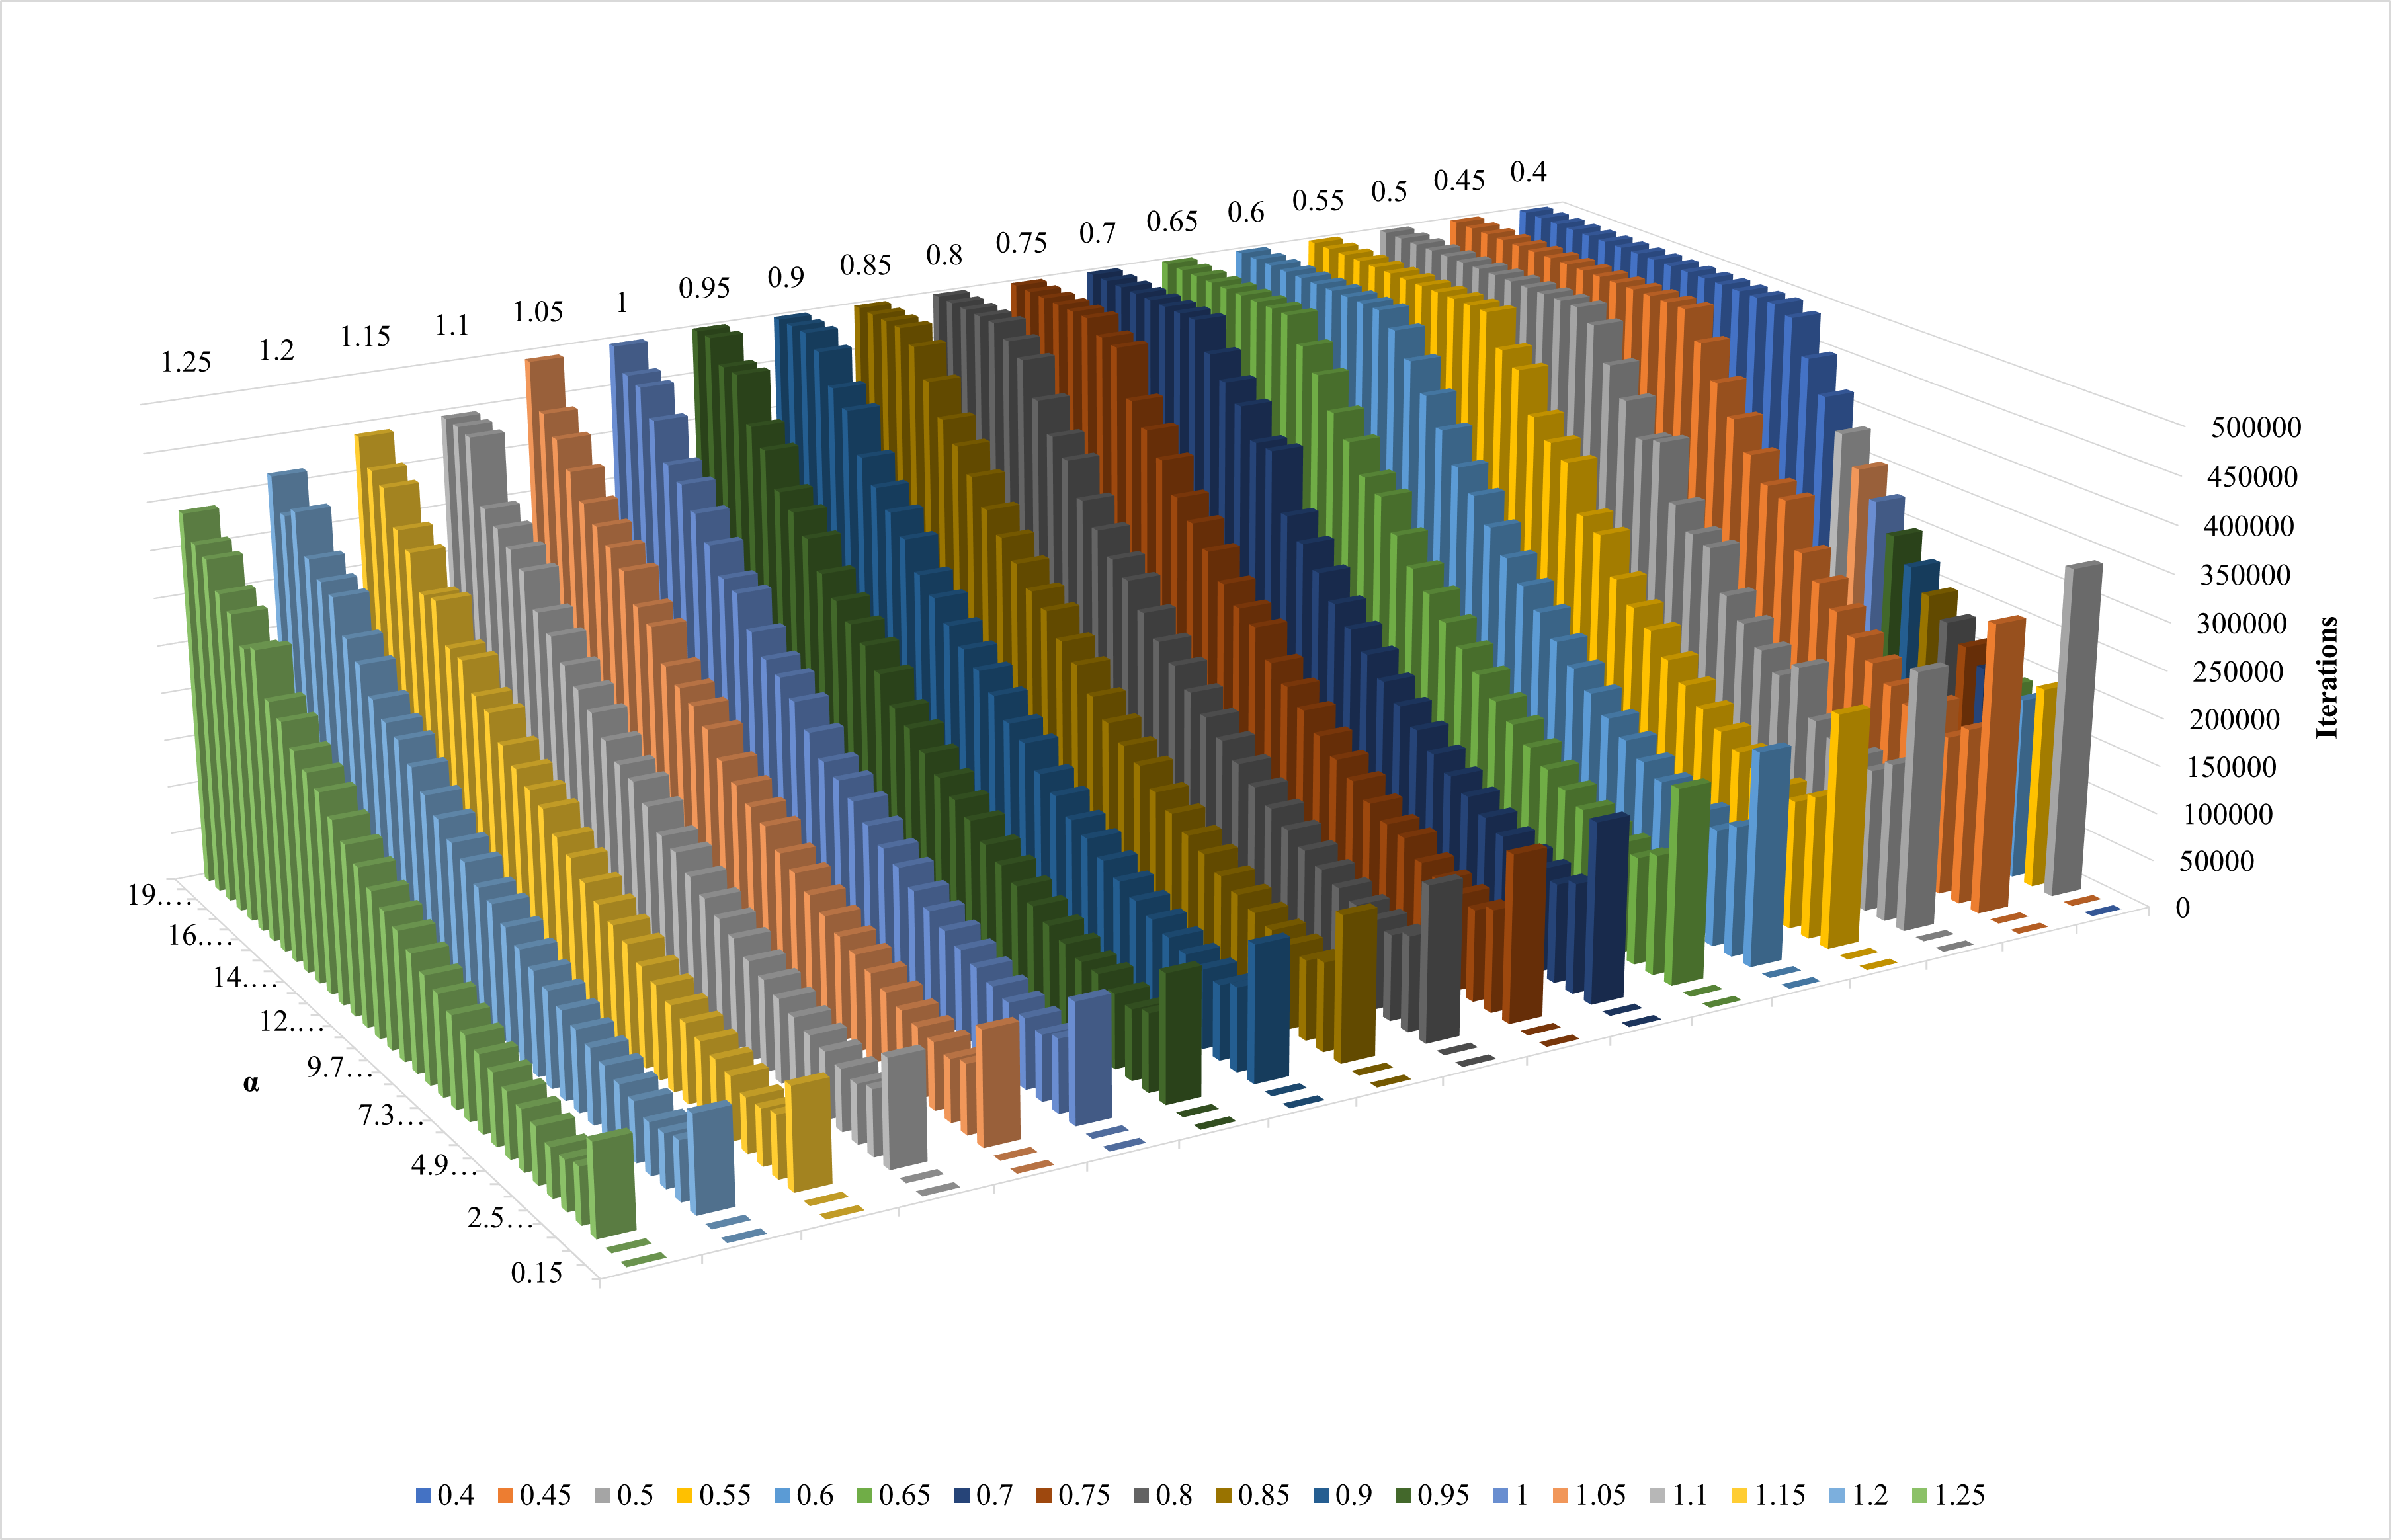
\includegraphics[scale=.55]{Iter-eps001-d1.png}
\end{center}
\caption{Number of iterations for $b_1$ and $\varepsilon=0.01$, w.r.t. $\alpha$ and $s$.}\label{res_iter001d1}
\end{figure}
\begin{figure}
\begin{center}
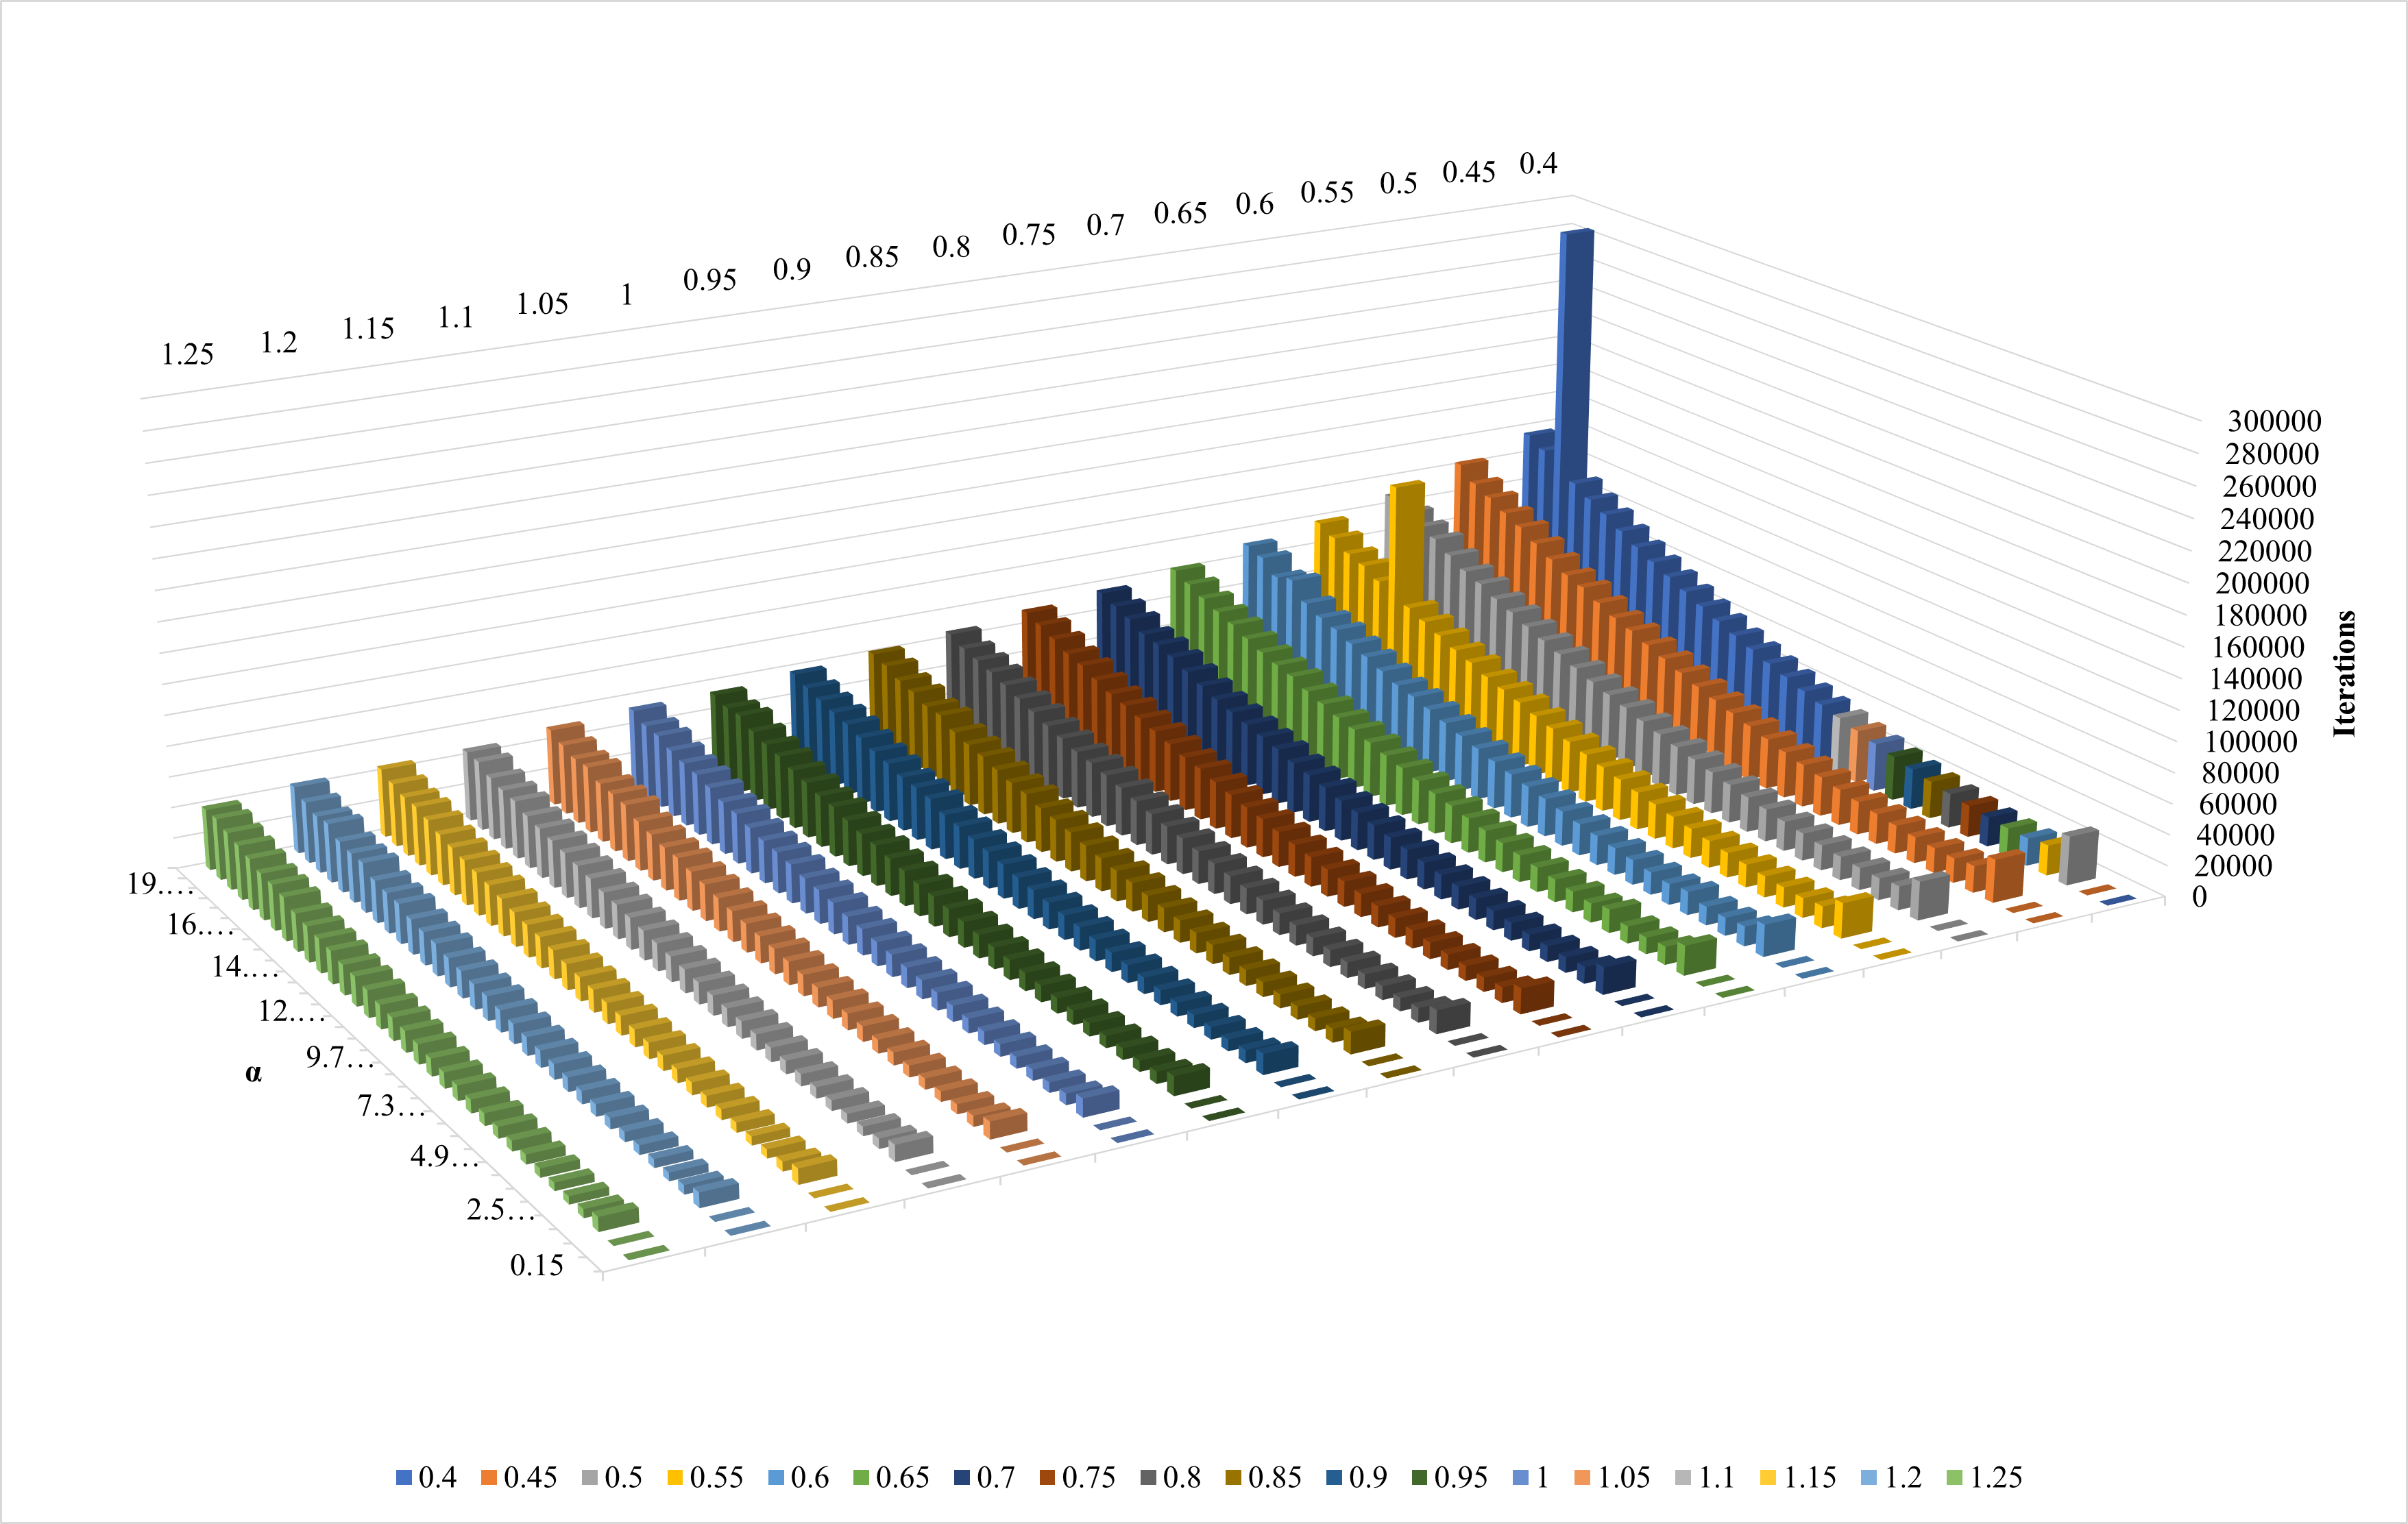
\includegraphics[scale=.55]{Iter-eps01-d1.png}
\end{center}
\caption{Number of iterations for $b_1$ and $\varepsilon=0.1$, w.r.t. $\alpha$ and $s$.}\label{res_iter01d1}
\end{figure}
\begin{figure}
\begin{center}
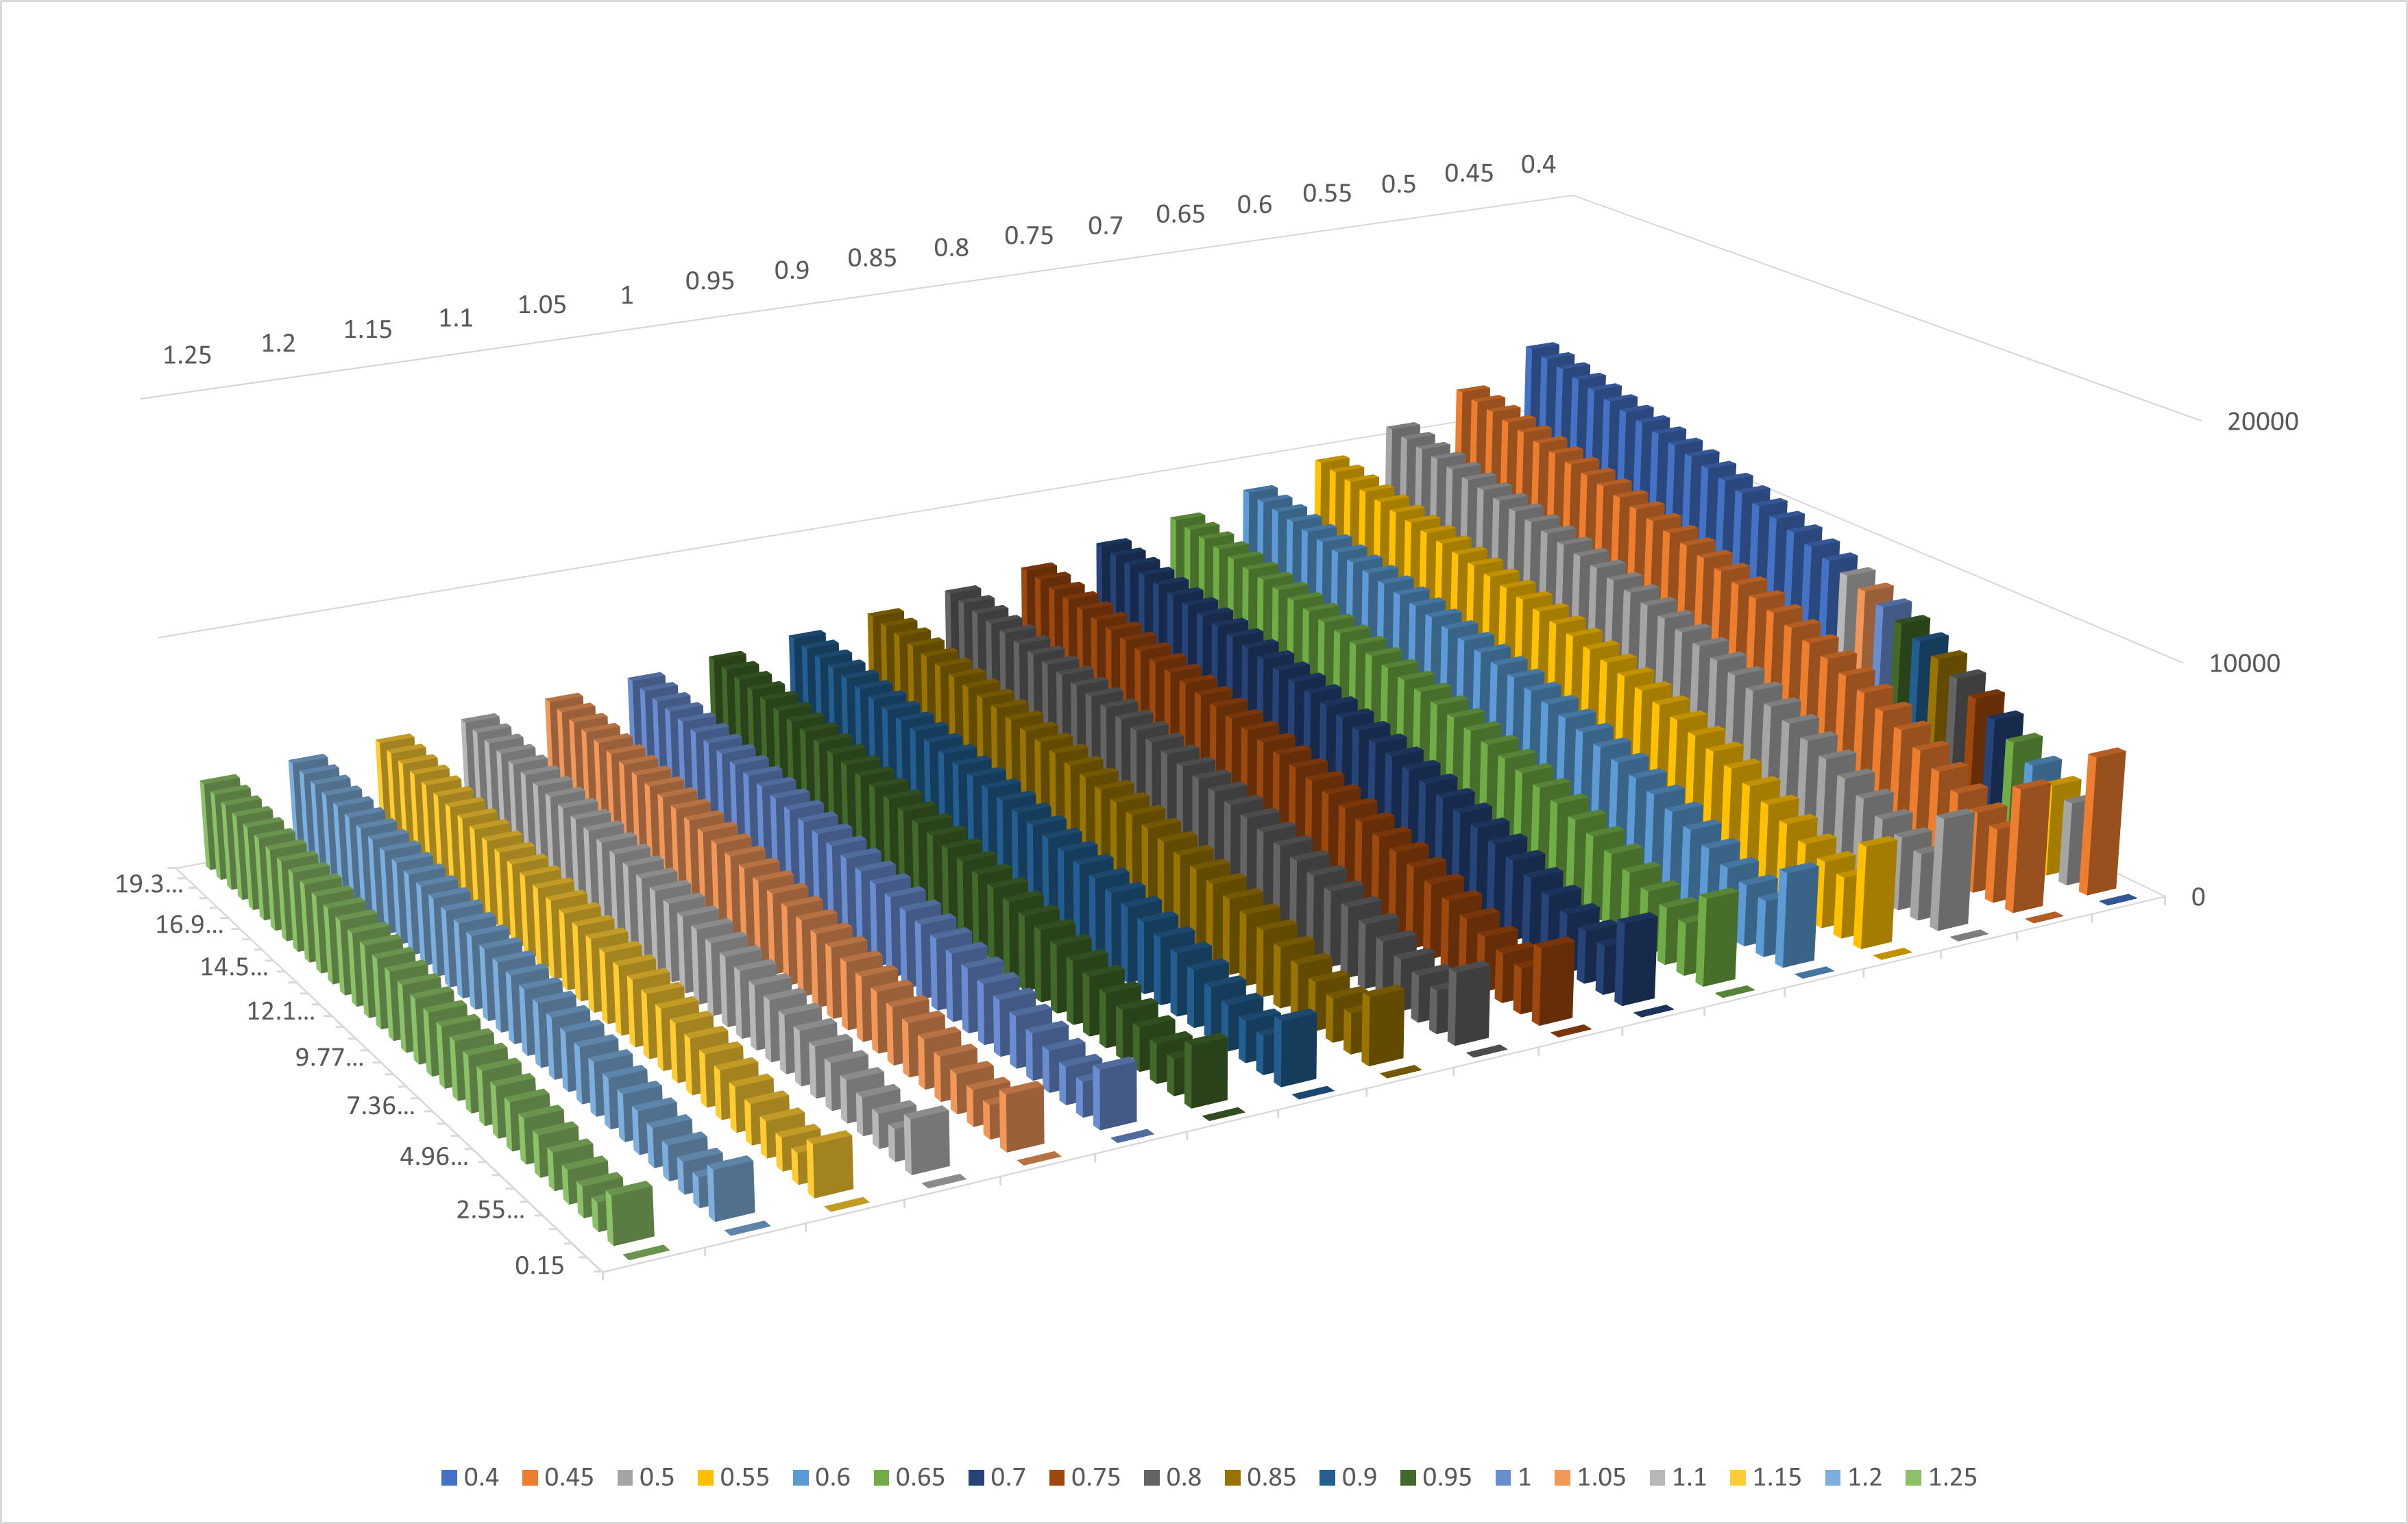
\includegraphics[scale=.55]{Iter-eps01-d2.png} 
\end{center}
\caption{Number of iterations for $b_2$ and $\varepsilon=0.1$, w.r.t. $\alpha$ and $s$.}\label{res_iter01d2}
\end{figure}


\section{Potential Threshold Cut Optimality}
The optimality of the cut that is induced by the potentials of \texttt{AlmostRoute} according to $\Phi(f)\leq (1+\varepsilon)\frac{b^Tv}{\Vert CB^Tv\Vert_1} $ with $v=R^T\nabla lmax(2\alpha R(b-Bf))$ was valid for all test runs with $\alpha>1.353$. Results for this congestion metric are shown in Figures \ref{res_lc01d1} and \ref{res_lc001d1} for $b_1$ with $\varepsilon=0.01$ and $\varepsilon=0.1$.
\begin{figure}
\begin{center}
\subfigure[$\frac{b^Tv}{\Vert CB^Tv\Vert_1}$.]{
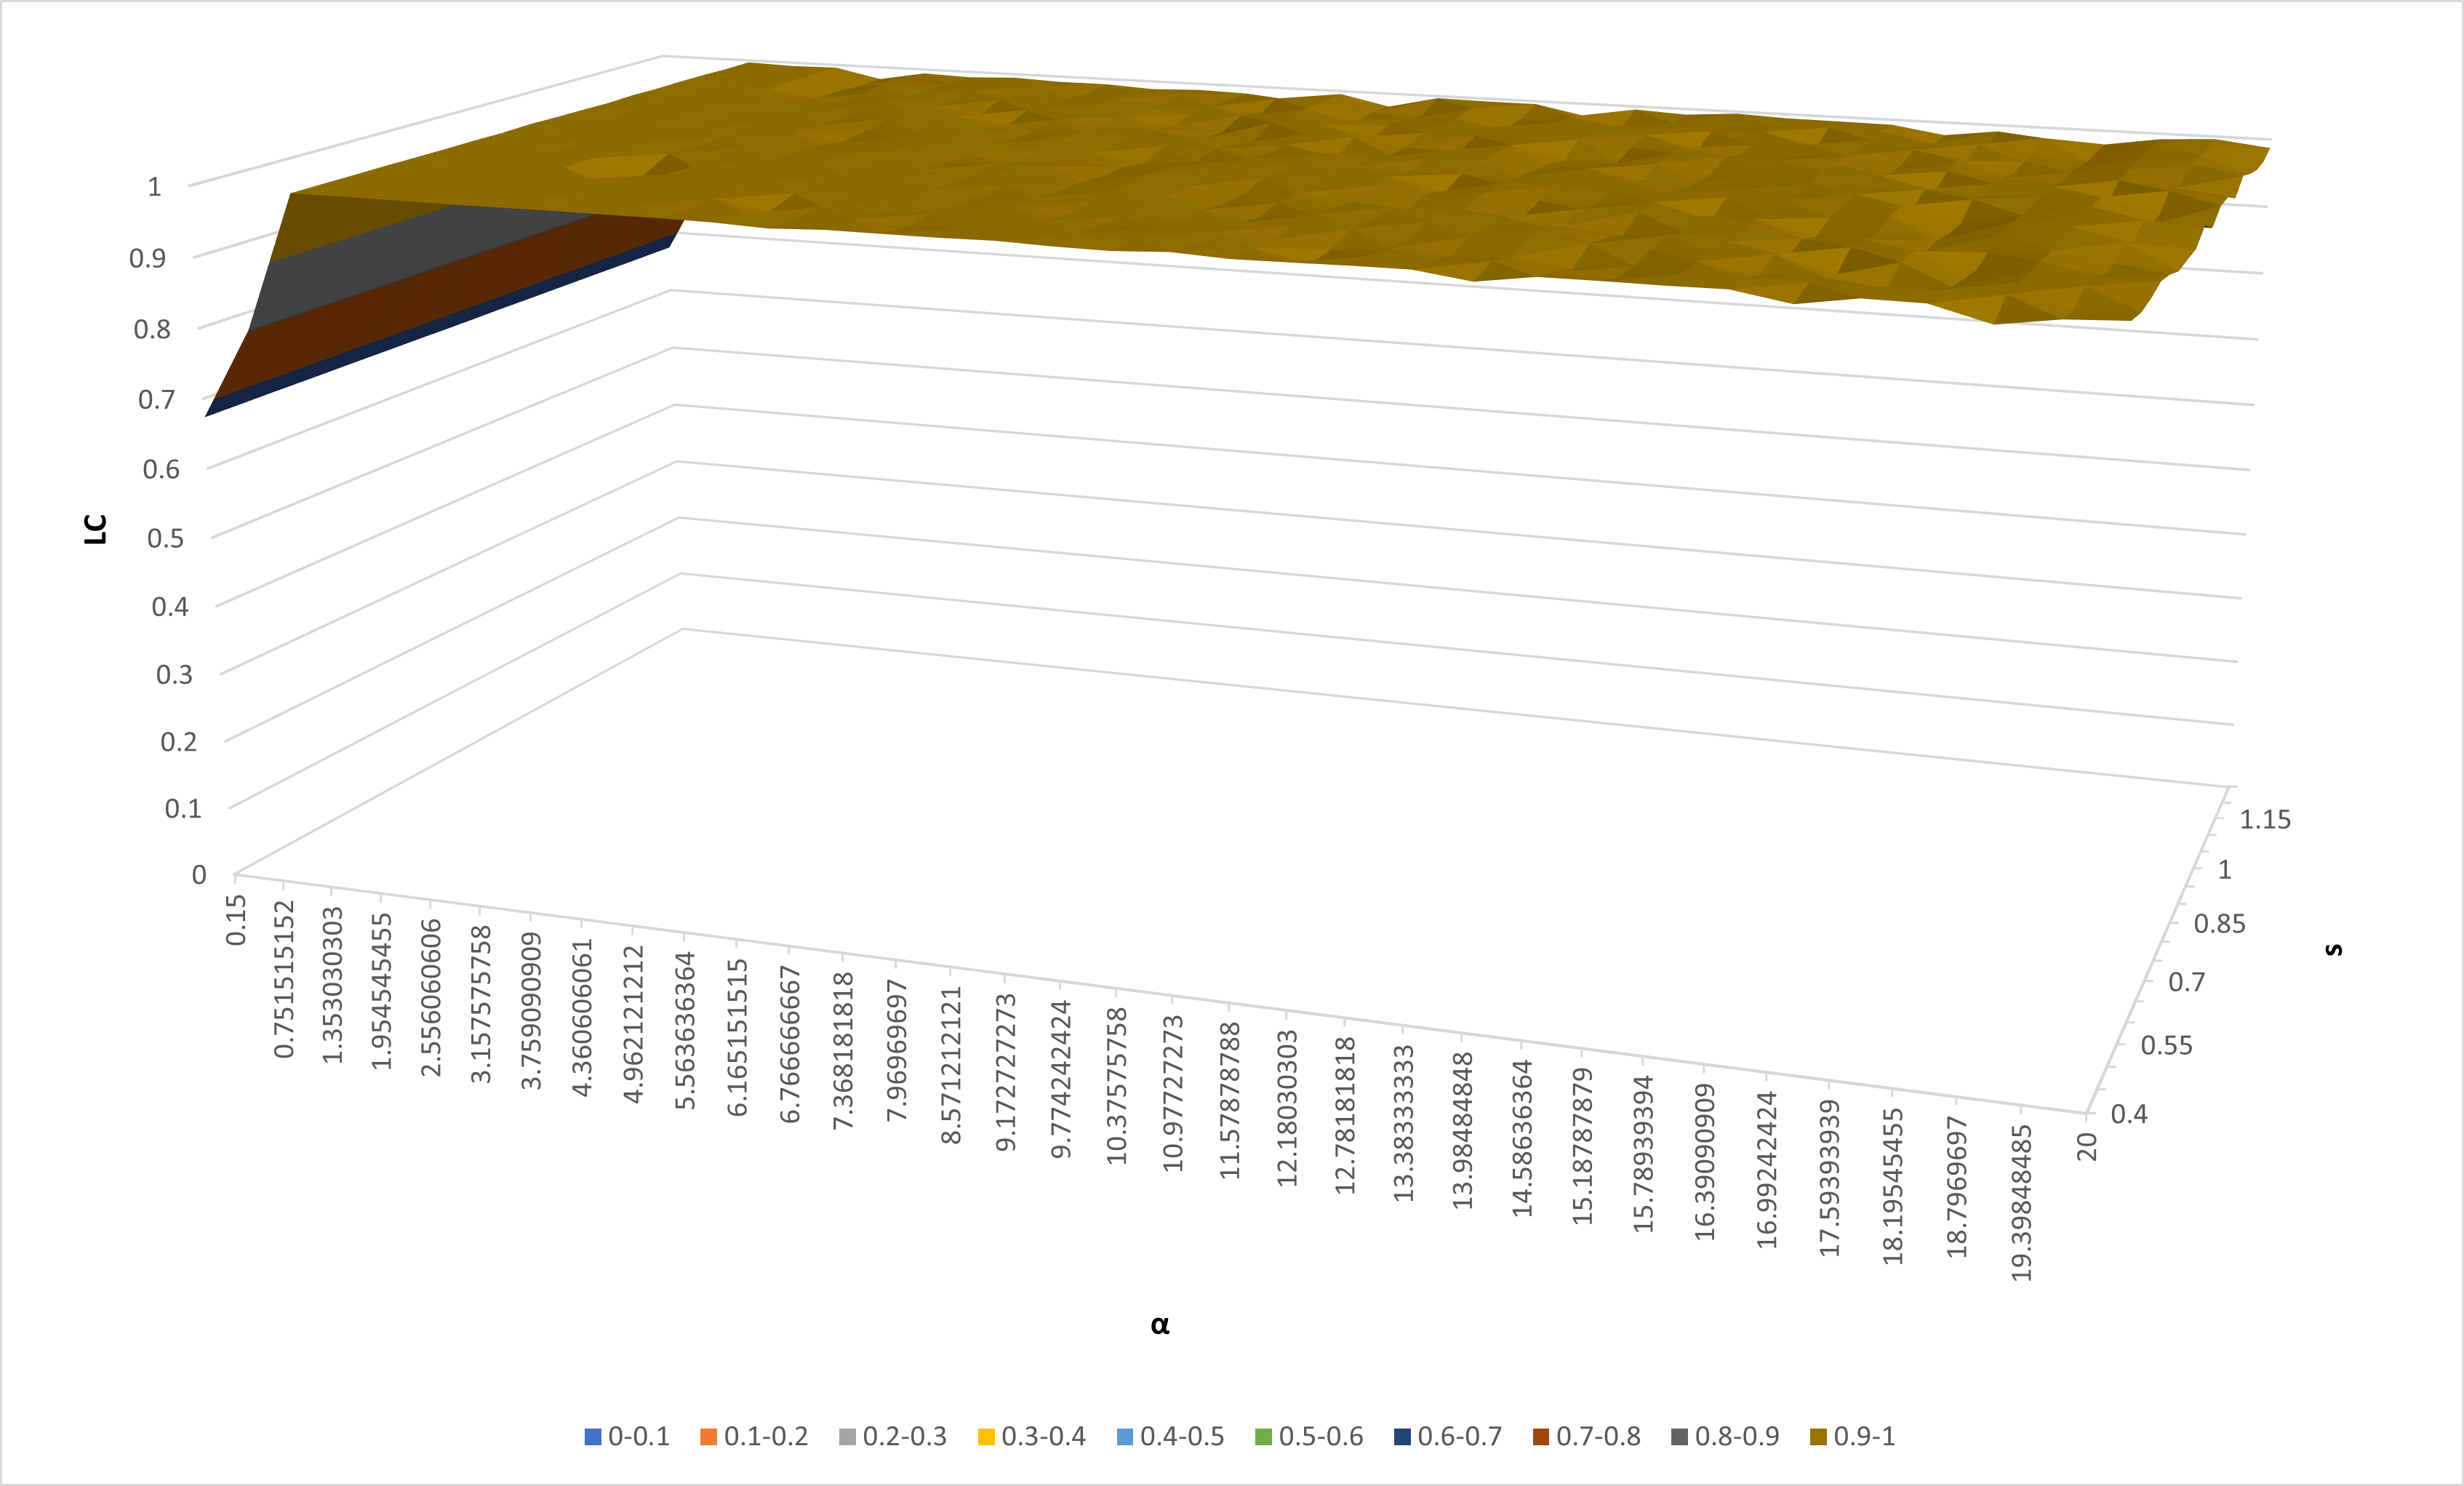
\includegraphics[scale=.55]{LC-eps01-d1.png}
}
\subfigure[$(1+\varepsilon)\frac{b^Tv}{\Vert CB^Tv\Vert_1}$.]{
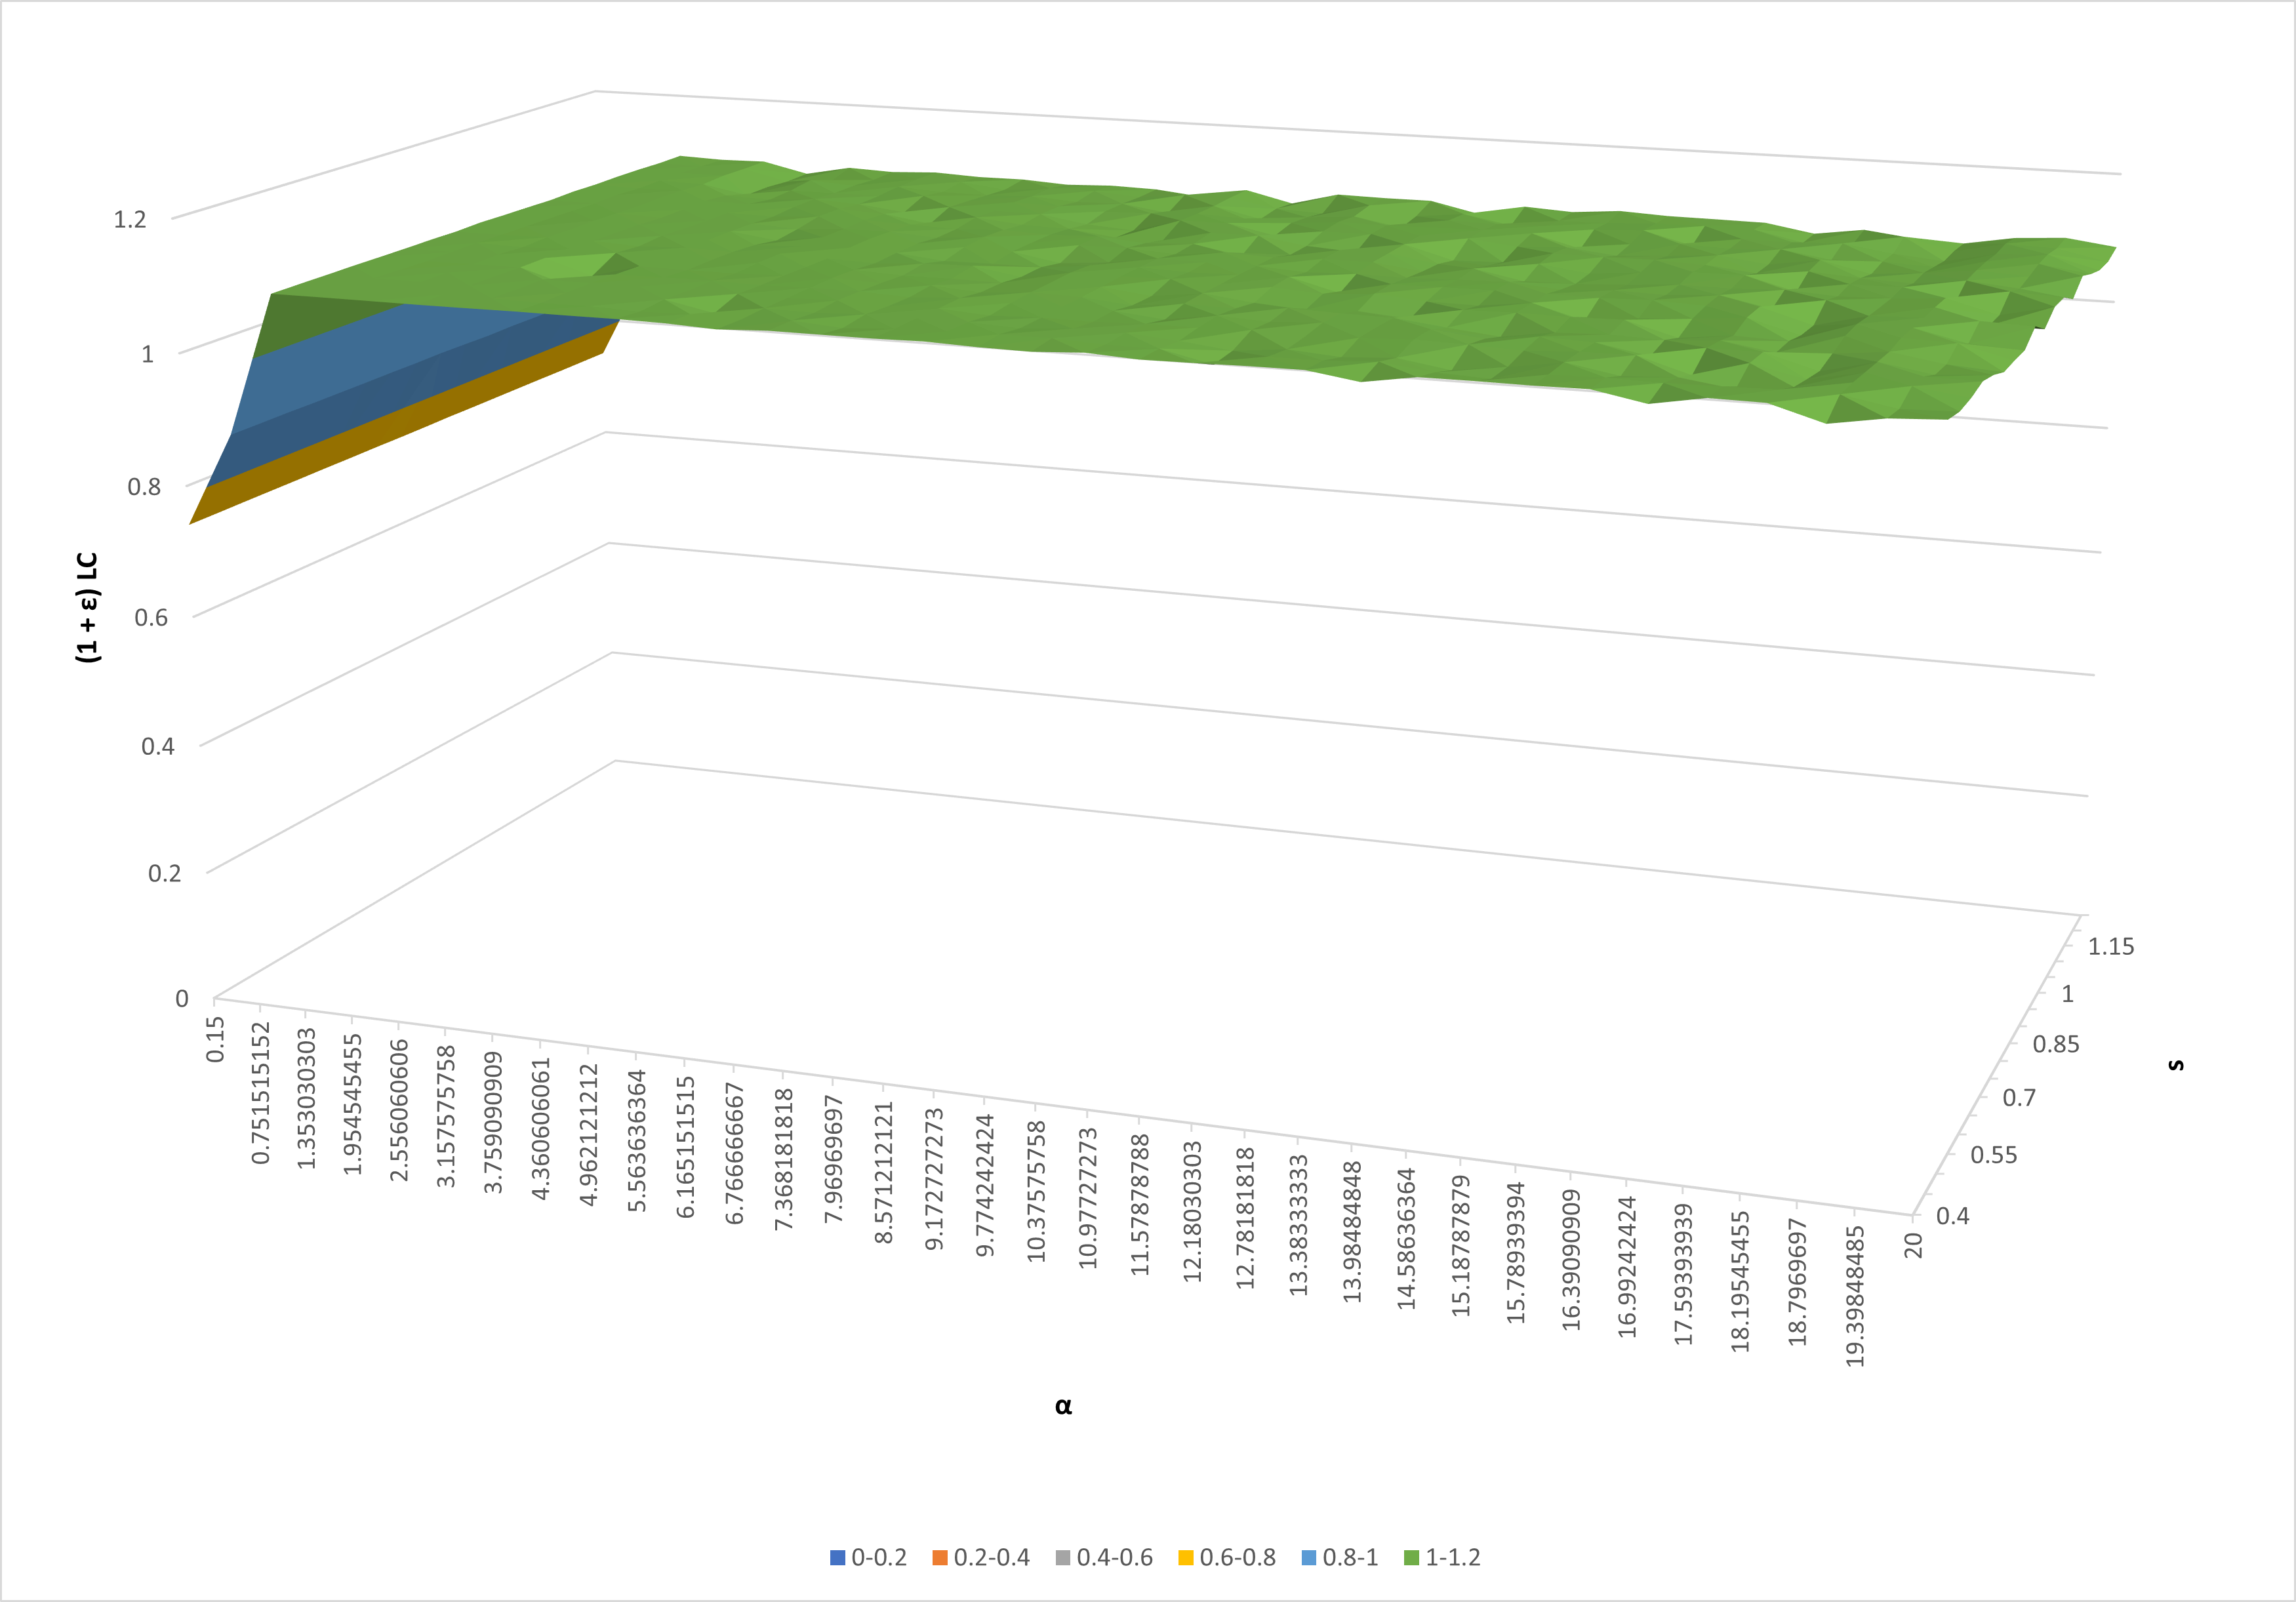
\includegraphics[scale=.55]{LCe-eps01-d1.png}
}
\end{center}
\caption{$\frac{b^Tv}{\Vert CB^Tv\Vert_1}$ and $(1+\varepsilon)\frac{b^Tv}{\Vert CB^Tv\Vert_1}$ for potentials $v$ after termination of $\texttt{AlmostRoute}(b_1,0.1)$. The optimal solution is $1$ and has to lie between both values.}\label{res_lc01d1}
\end{figure}
\begin{figure}
\begin{center}
\subfigure[$\frac{b^Tv}{\Vert CB^Tv\Vert_1}$.]{
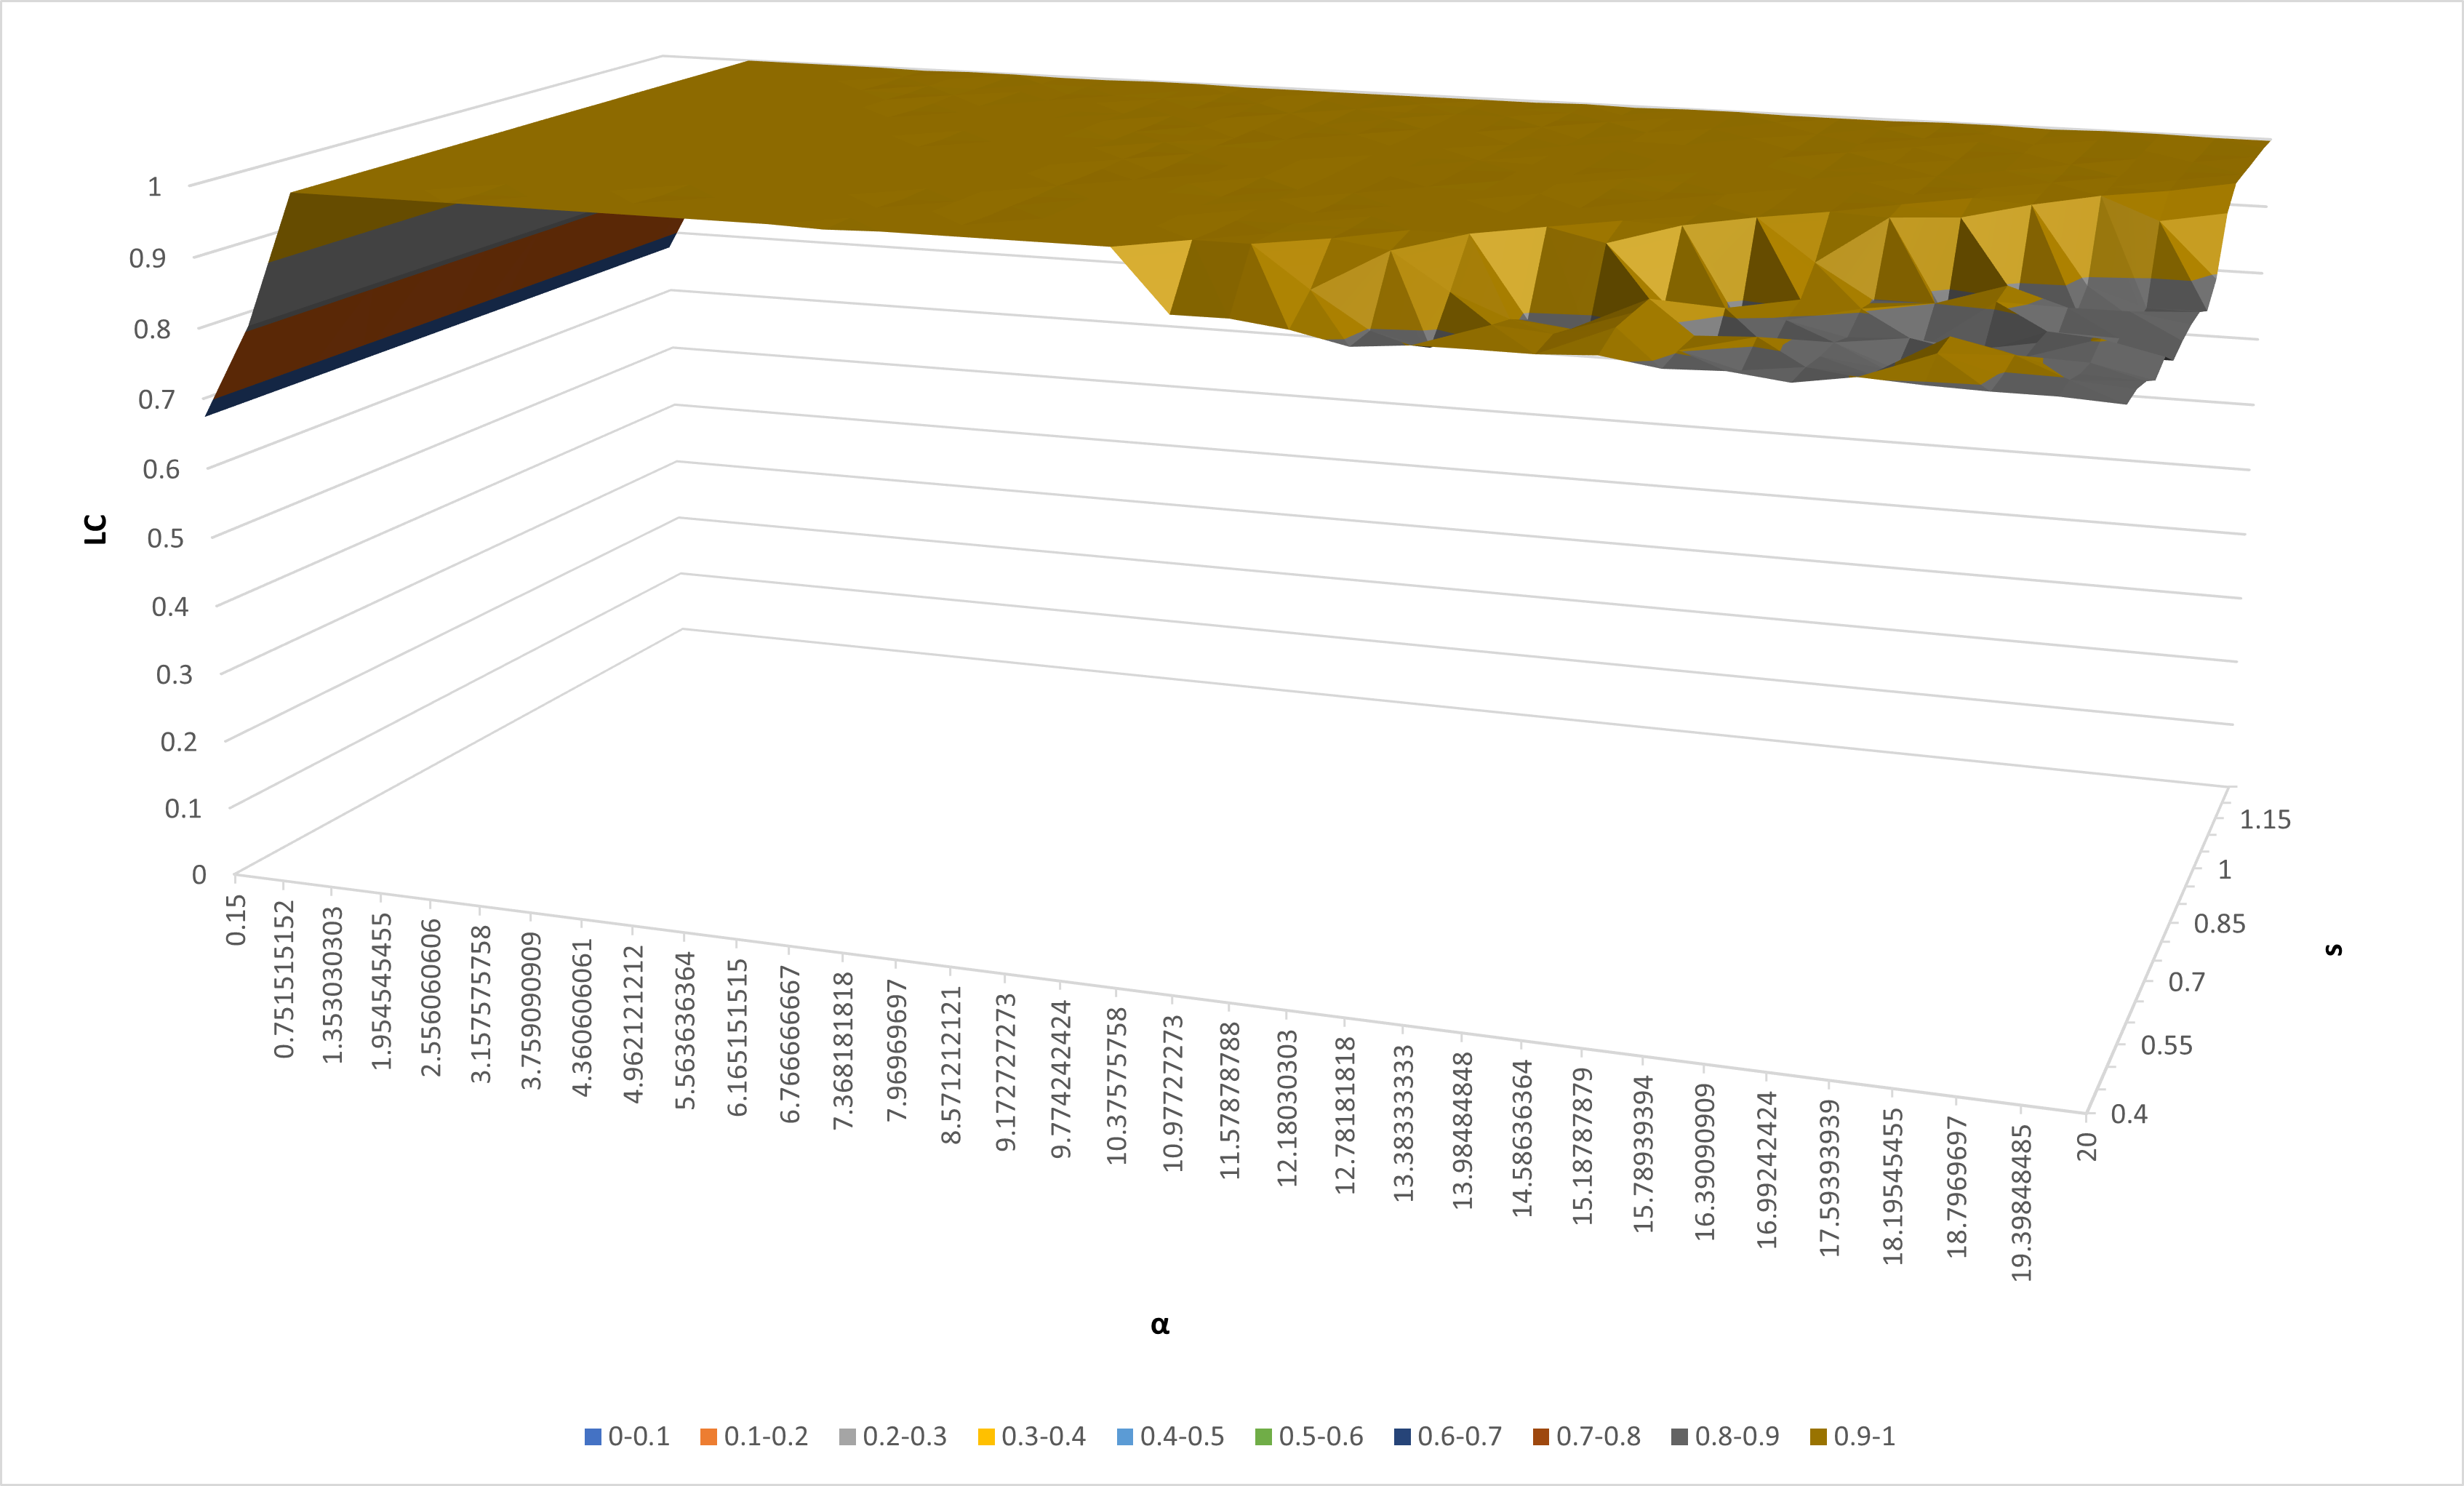
\includegraphics[scale=.55]{LC-eps001-d1.png}
}
\subfigure[$(1+\varepsilon)\frac{b^Tv}{\Vert CB^Tv\Vert_1}$.]{
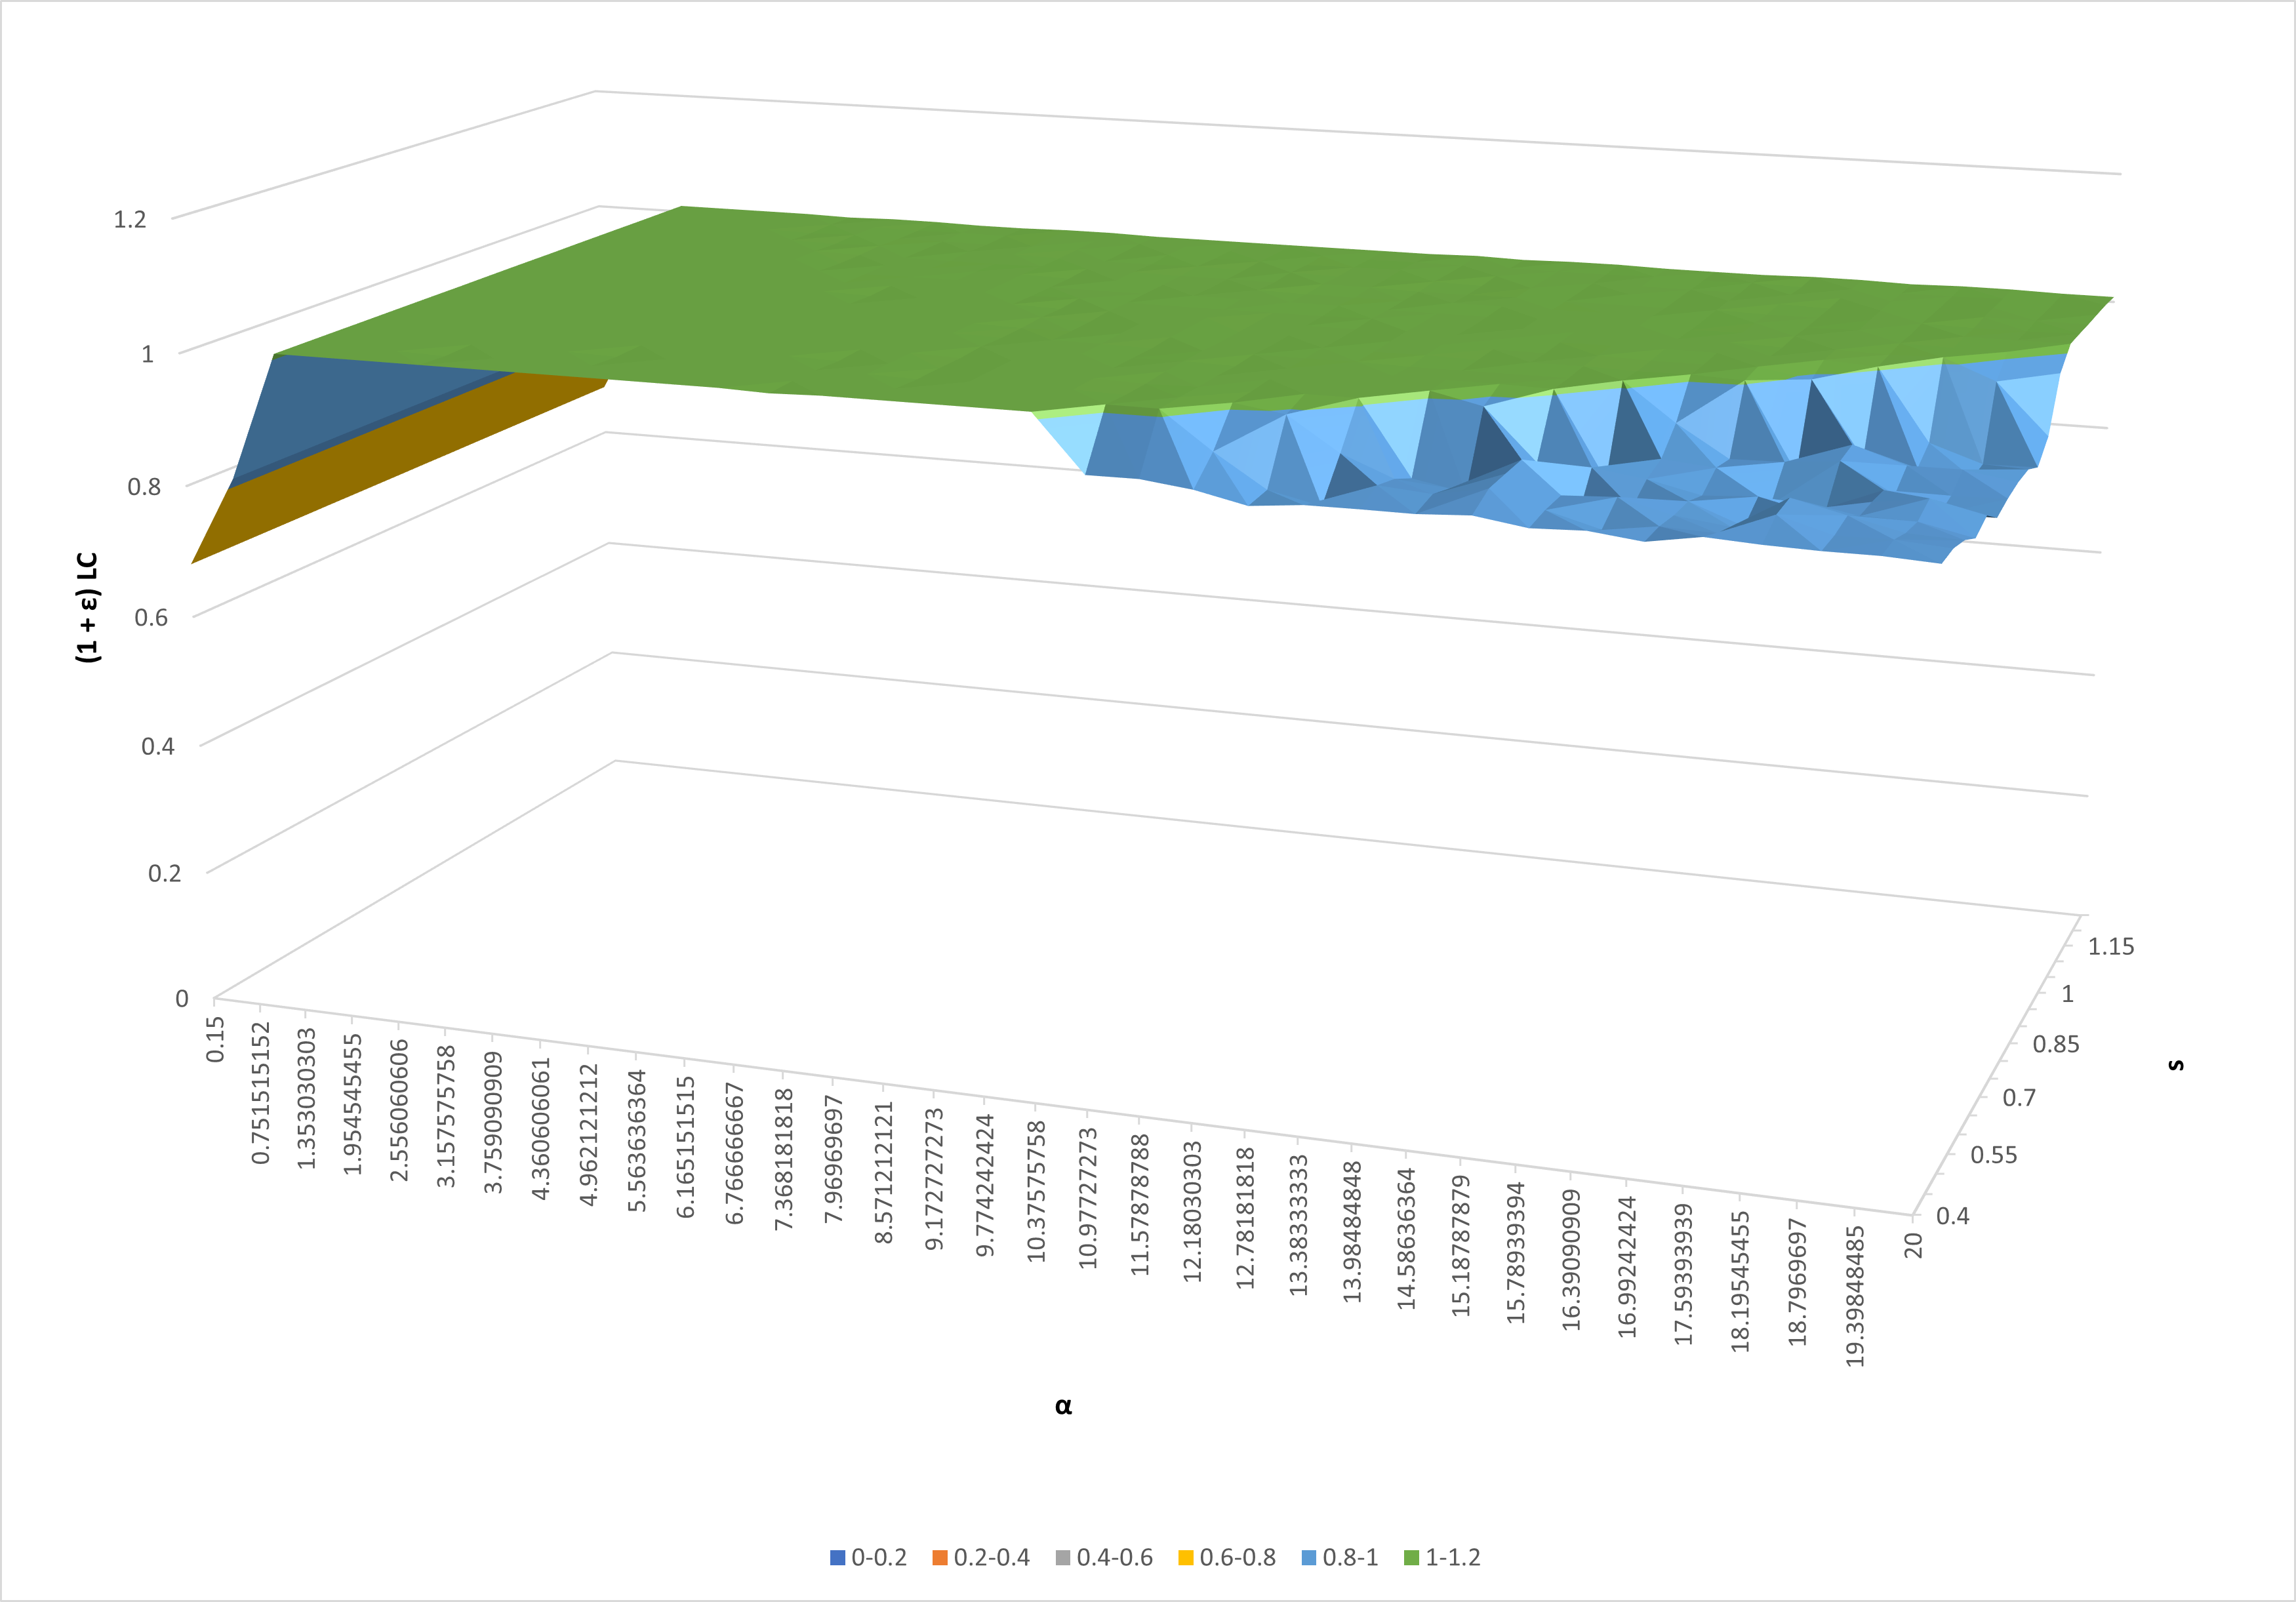
\includegraphics[scale=.55]{LCe-eps001-d1.png}
}
\end{center}
\caption{$\frac{b^Tv}{\Vert CB^Tv\Vert_1}$ and $(1+\varepsilon)\frac{b^Tv}{\Vert CB^Tv\Vert_1}$ for potentials $v$ after termination of $\texttt{AlmostRoute}(b_1,0.01)$. The optimal solution is $1$ and has to lie between both values. Note that the results from runs that took $500,000$ iterations should be ignored here, as the iteration was prematurely terminated. See Figure \ref{res_iter001d1} for iterations.}\label{res_lc001d1}
\end{figure}

\section{Step Size Optimization}
The step size optimization showed significant iteration and runtime improvements, even for our simple implementations of the ternary search and the golden section search. The runtime and iterations were slightly better with golden section search compared to ternary search for most runs, and sometimes significantly better.\\
Comparisons between an unoptimized run and runs with golden section search are shown in Figures \ref{res_gss001d1}, \ref{res_gss001d2} and \ref{res_gss01d1}.
\begin{figure}
\begin{center}
\subfigure[Comparison of iterations.]{
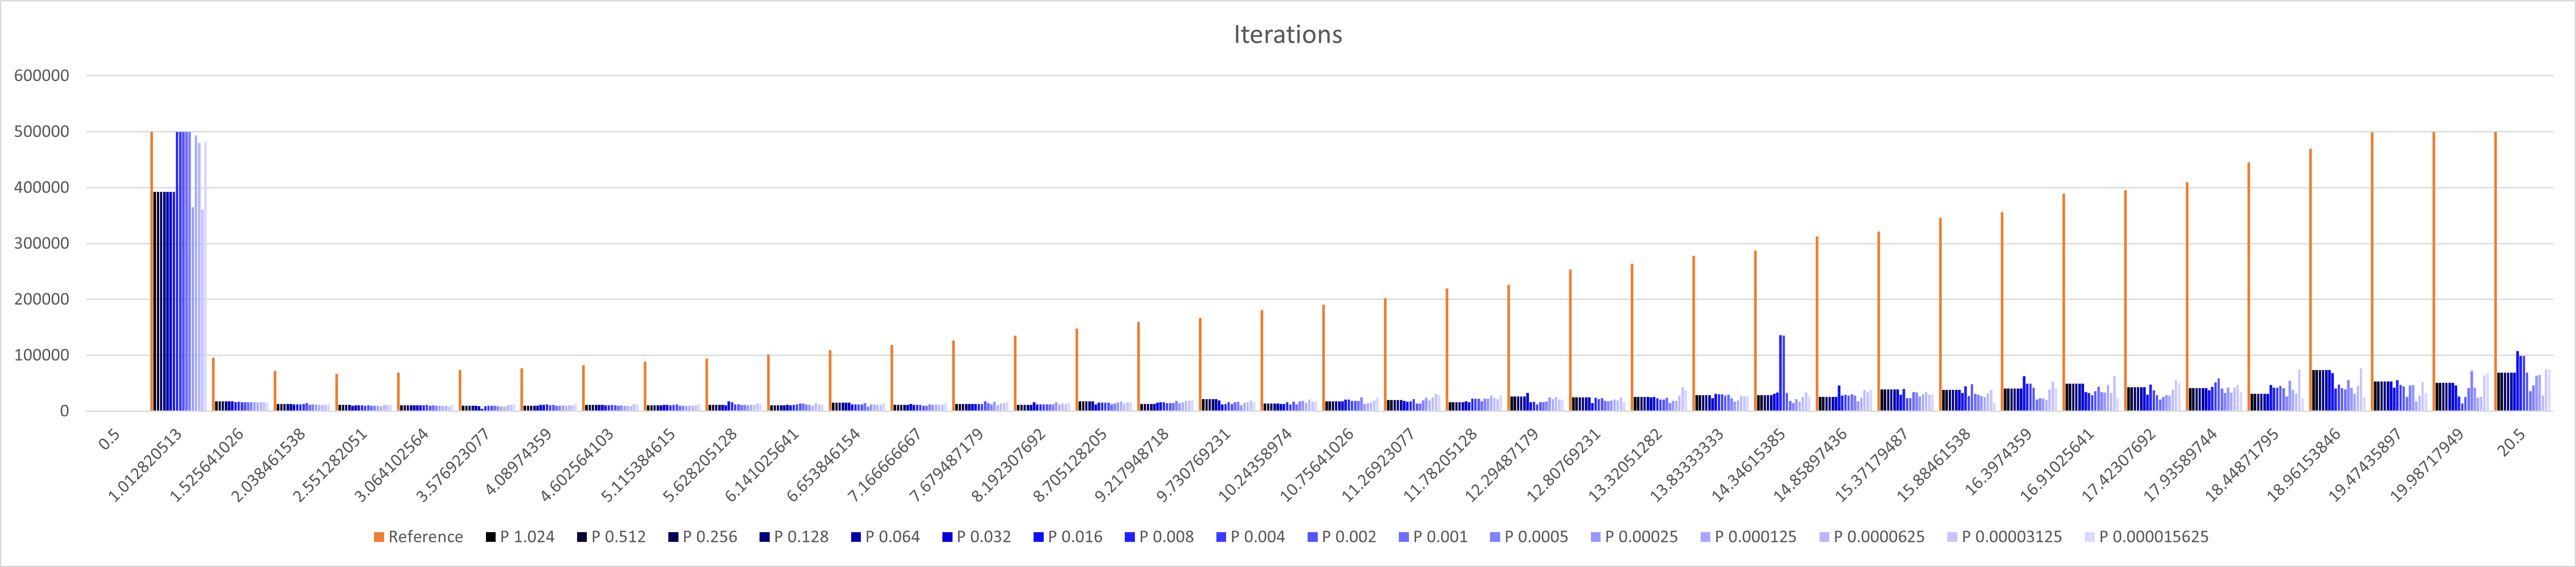
\includegraphics[scale=.35]{Iter-GSS-eps001-d1.png}
}
\subfigure[Comparisons of runtimes.]{
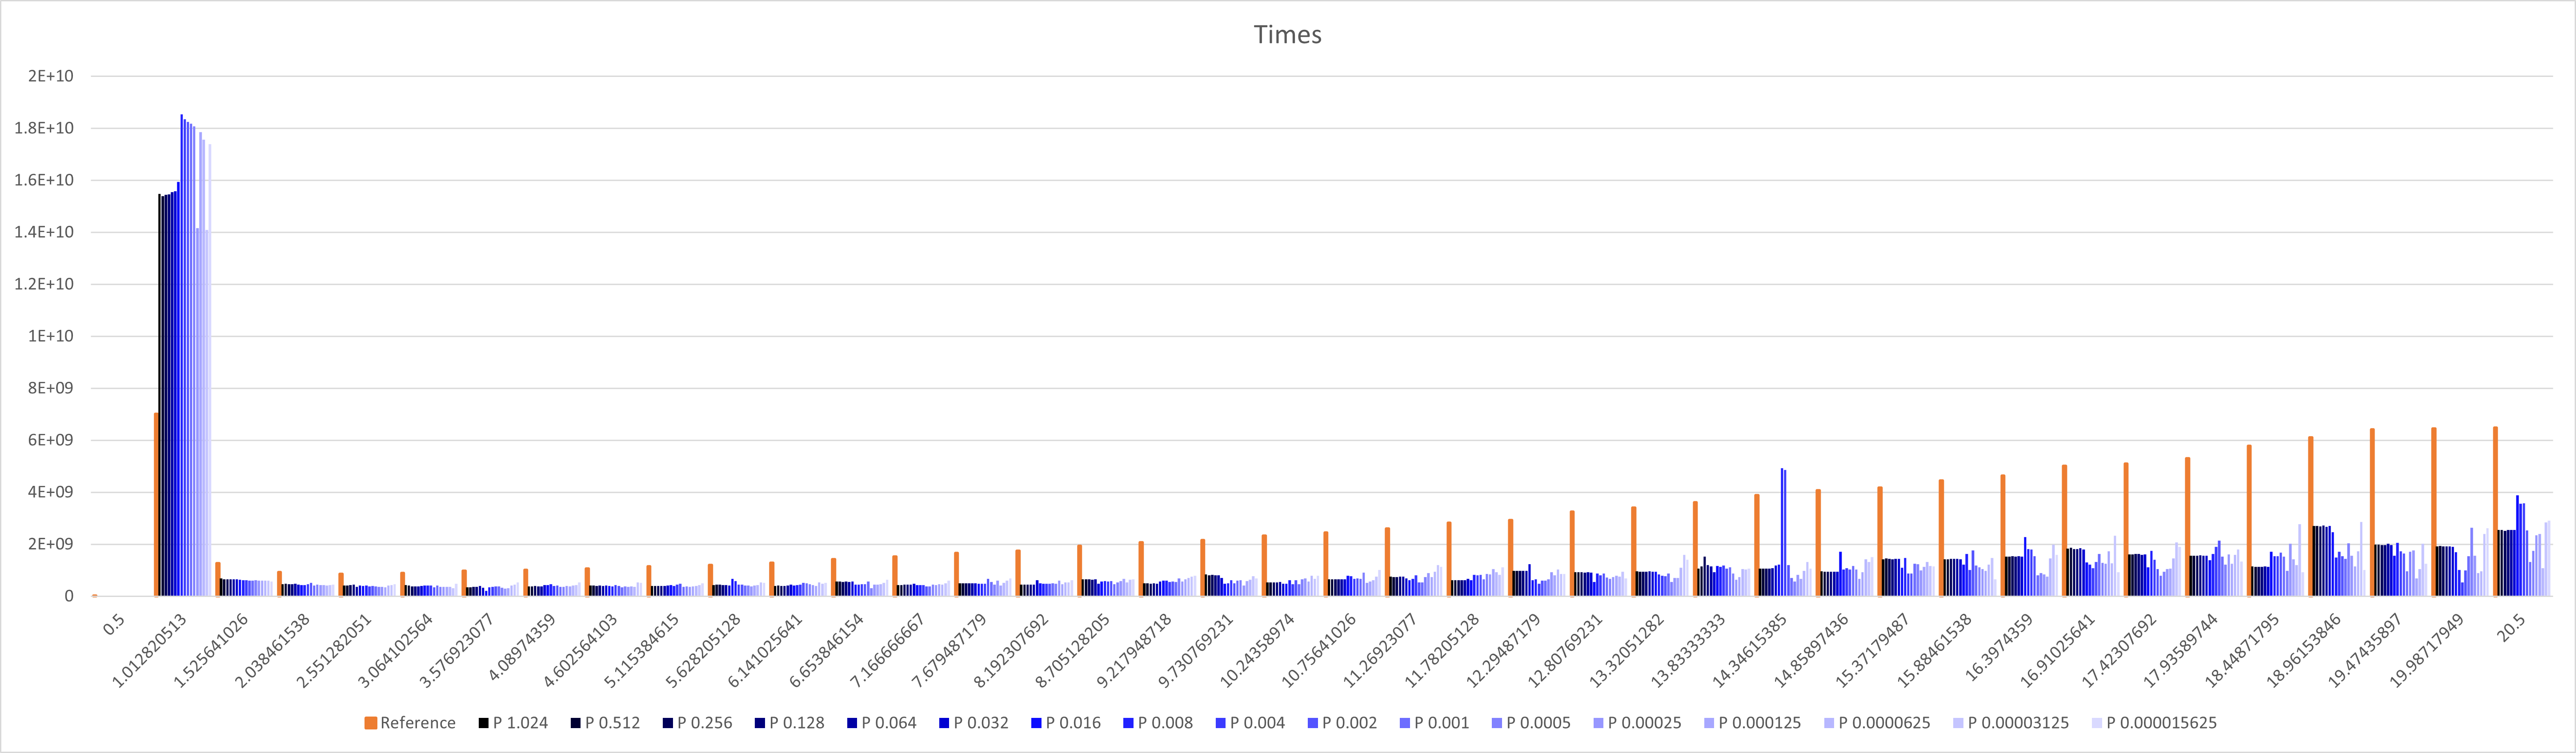
\includegraphics[scale=.35]{Times-GSS-eps001-d1.png}
}
\end{center}
\caption{Comparison of iterations and runtimes between naive steepest descent and golden section search optimization for $b_1$ and $\varepsilon=0.01$.}\label{res_gss001d1}
\end{figure}
\begin{figure}
\begin{center}
\subfigure[Comparison of iterations.]{
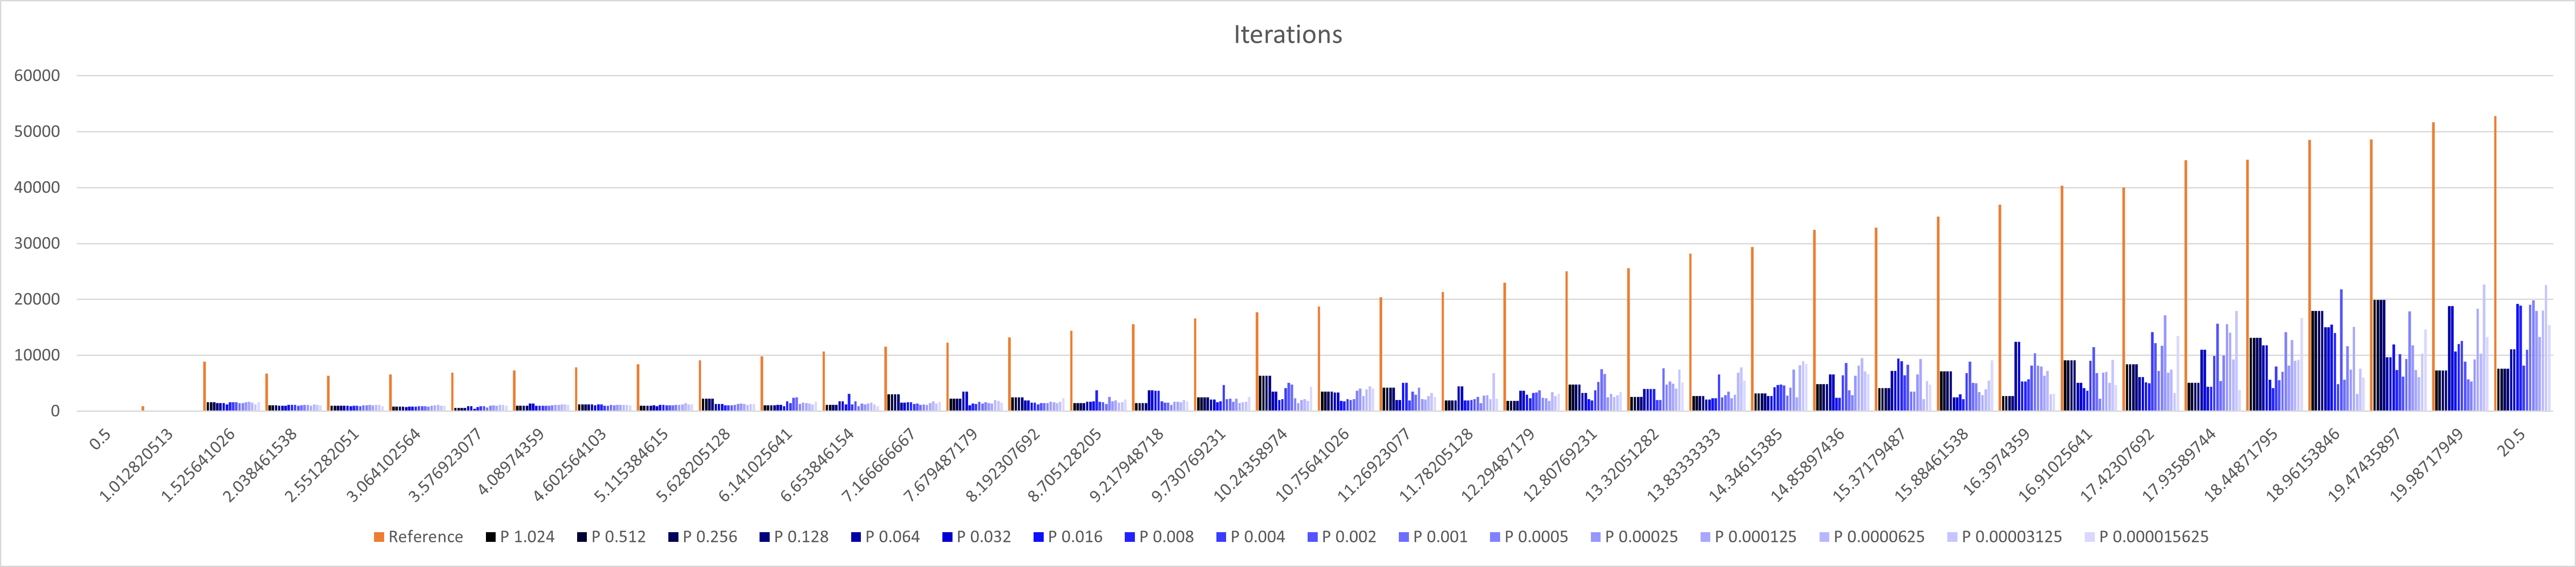
\includegraphics[scale=.35]{Iter-GSS-eps01-d1.png}
}
\subfigure[Comparisons of runtimes.]{
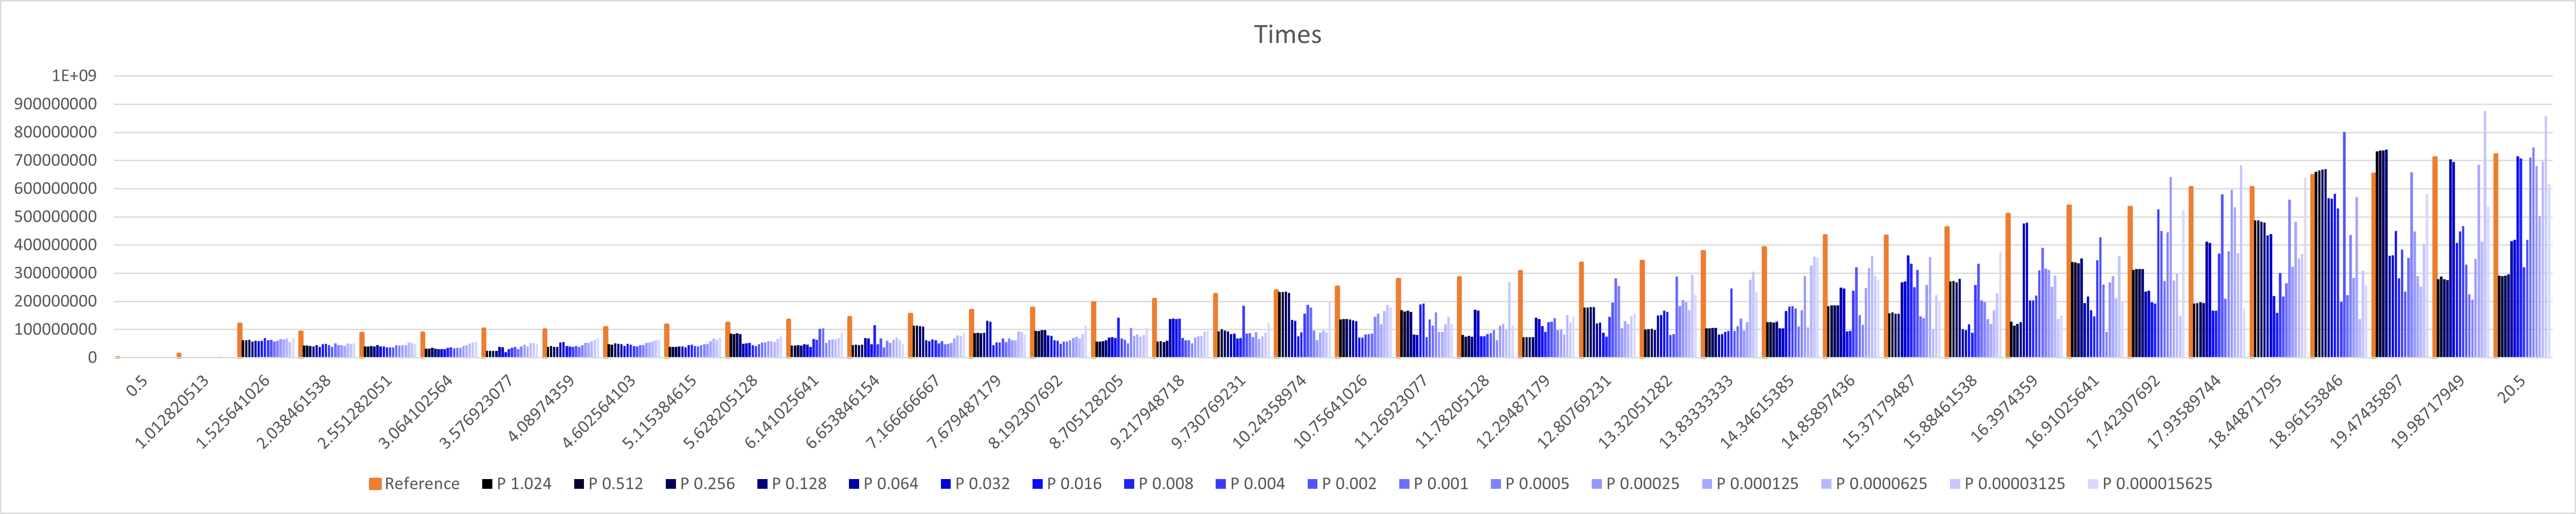
\includegraphics[scale=.35]{Times-GSS-eps01-d1.png}
}
\end{center}
\caption{Comparison of iterations and runtimes between naive steepest descent and golden section search optimization for $b_1$ and $\varepsilon=0.1$.}\label{res_gss01d1}
\end{figure}
\begin{figure}
\begin{center}
\subfigure[Comparison of iterations.]{
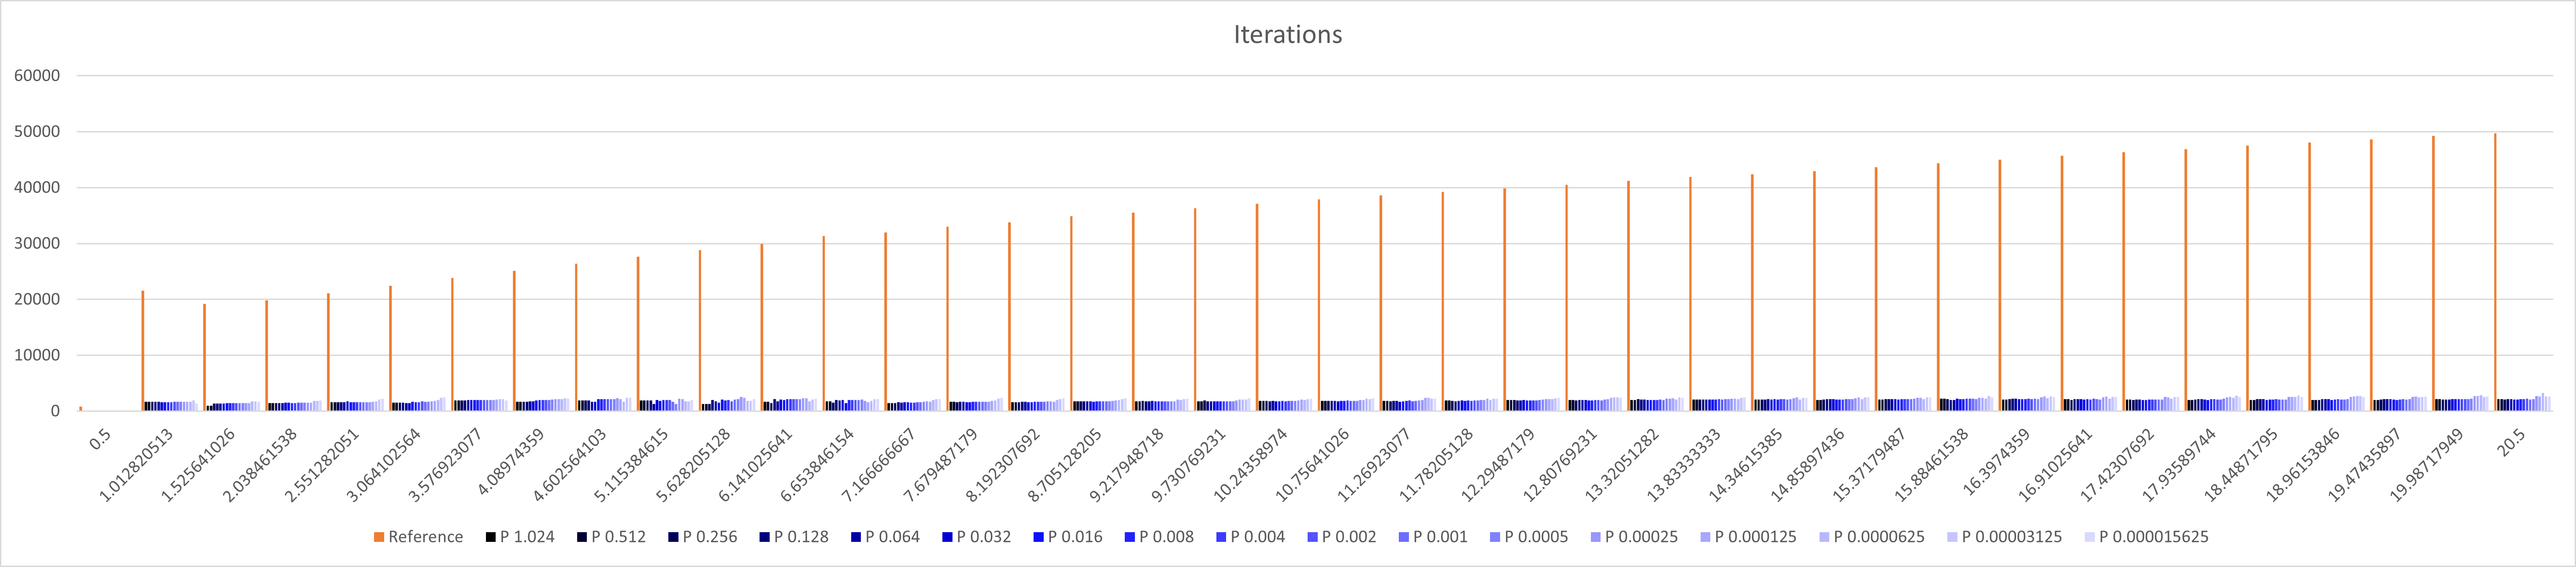
\includegraphics[scale=.35]{Iter-GSS-eps001-d2.png}
}
\subfigure[Comparisons of runtimes.]{
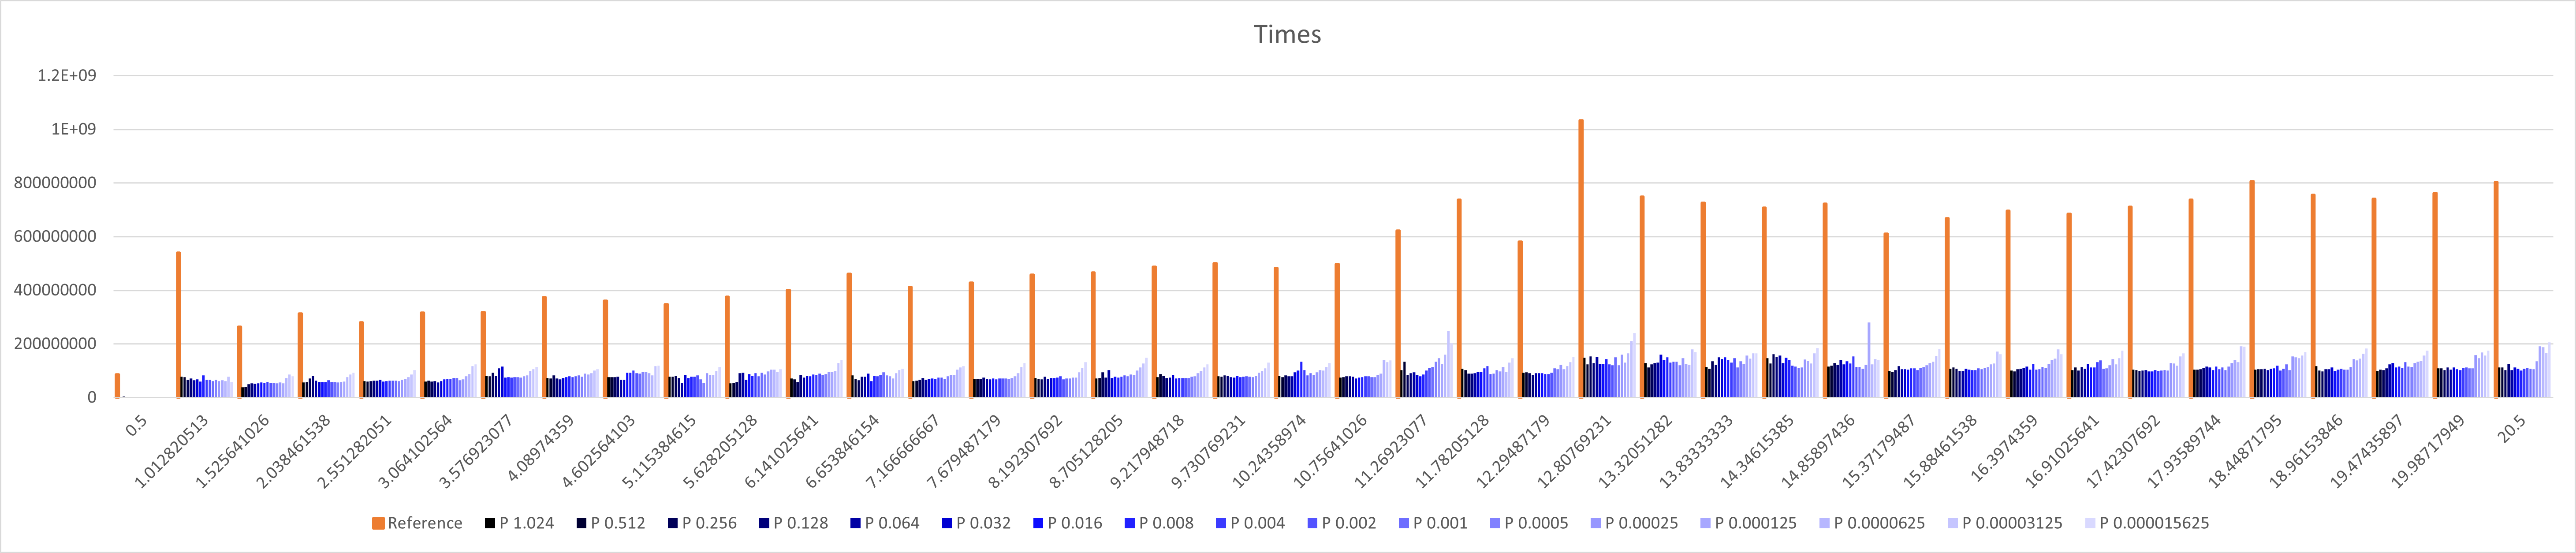
\includegraphics[scale=.35]{Times-GSS-eps001-d2.png}
}
\end{center}
\caption{Comparison of iterations and runtimes between naive steepest descent and golden section search optimization for $b_2$ and $\varepsilon=0.01$.}\label{res_gss001d2}
\end{figure}

\section{Empiric Search for $\alpha$}
For $d=1$, an extensive random sampling was performed. For millions of samples, the highest value of the sampled lower limits for $\alpha$ was outputted, condensed into a single data point. For the results, see Figure \ref{res_rsample}. As expected, $n=4,5$ have an approximator with $\alpha=1$.\\
Some smaller samplings with $\varsigma=0.02\cdot i$ and $1000$ samples for each $i\in[50]$ were also performed, outputting the value of the $\alpha$ estimate $\frac{\text{opt}(b)}{\Vert Rb\Vert_\infty}$ for each sample $b$. This gives a better overview on the distribution of this ratio. The results for $n\in\{4,8,16,32,64\}$ are shown in Figures \ref{res_rsample_4}, \ref{res_rsample_8}, \ref{res_rsample_16}, \ref{res_rsample_32} and \ref{res_rsample_64}.
\begin{figure}
\begin{center}
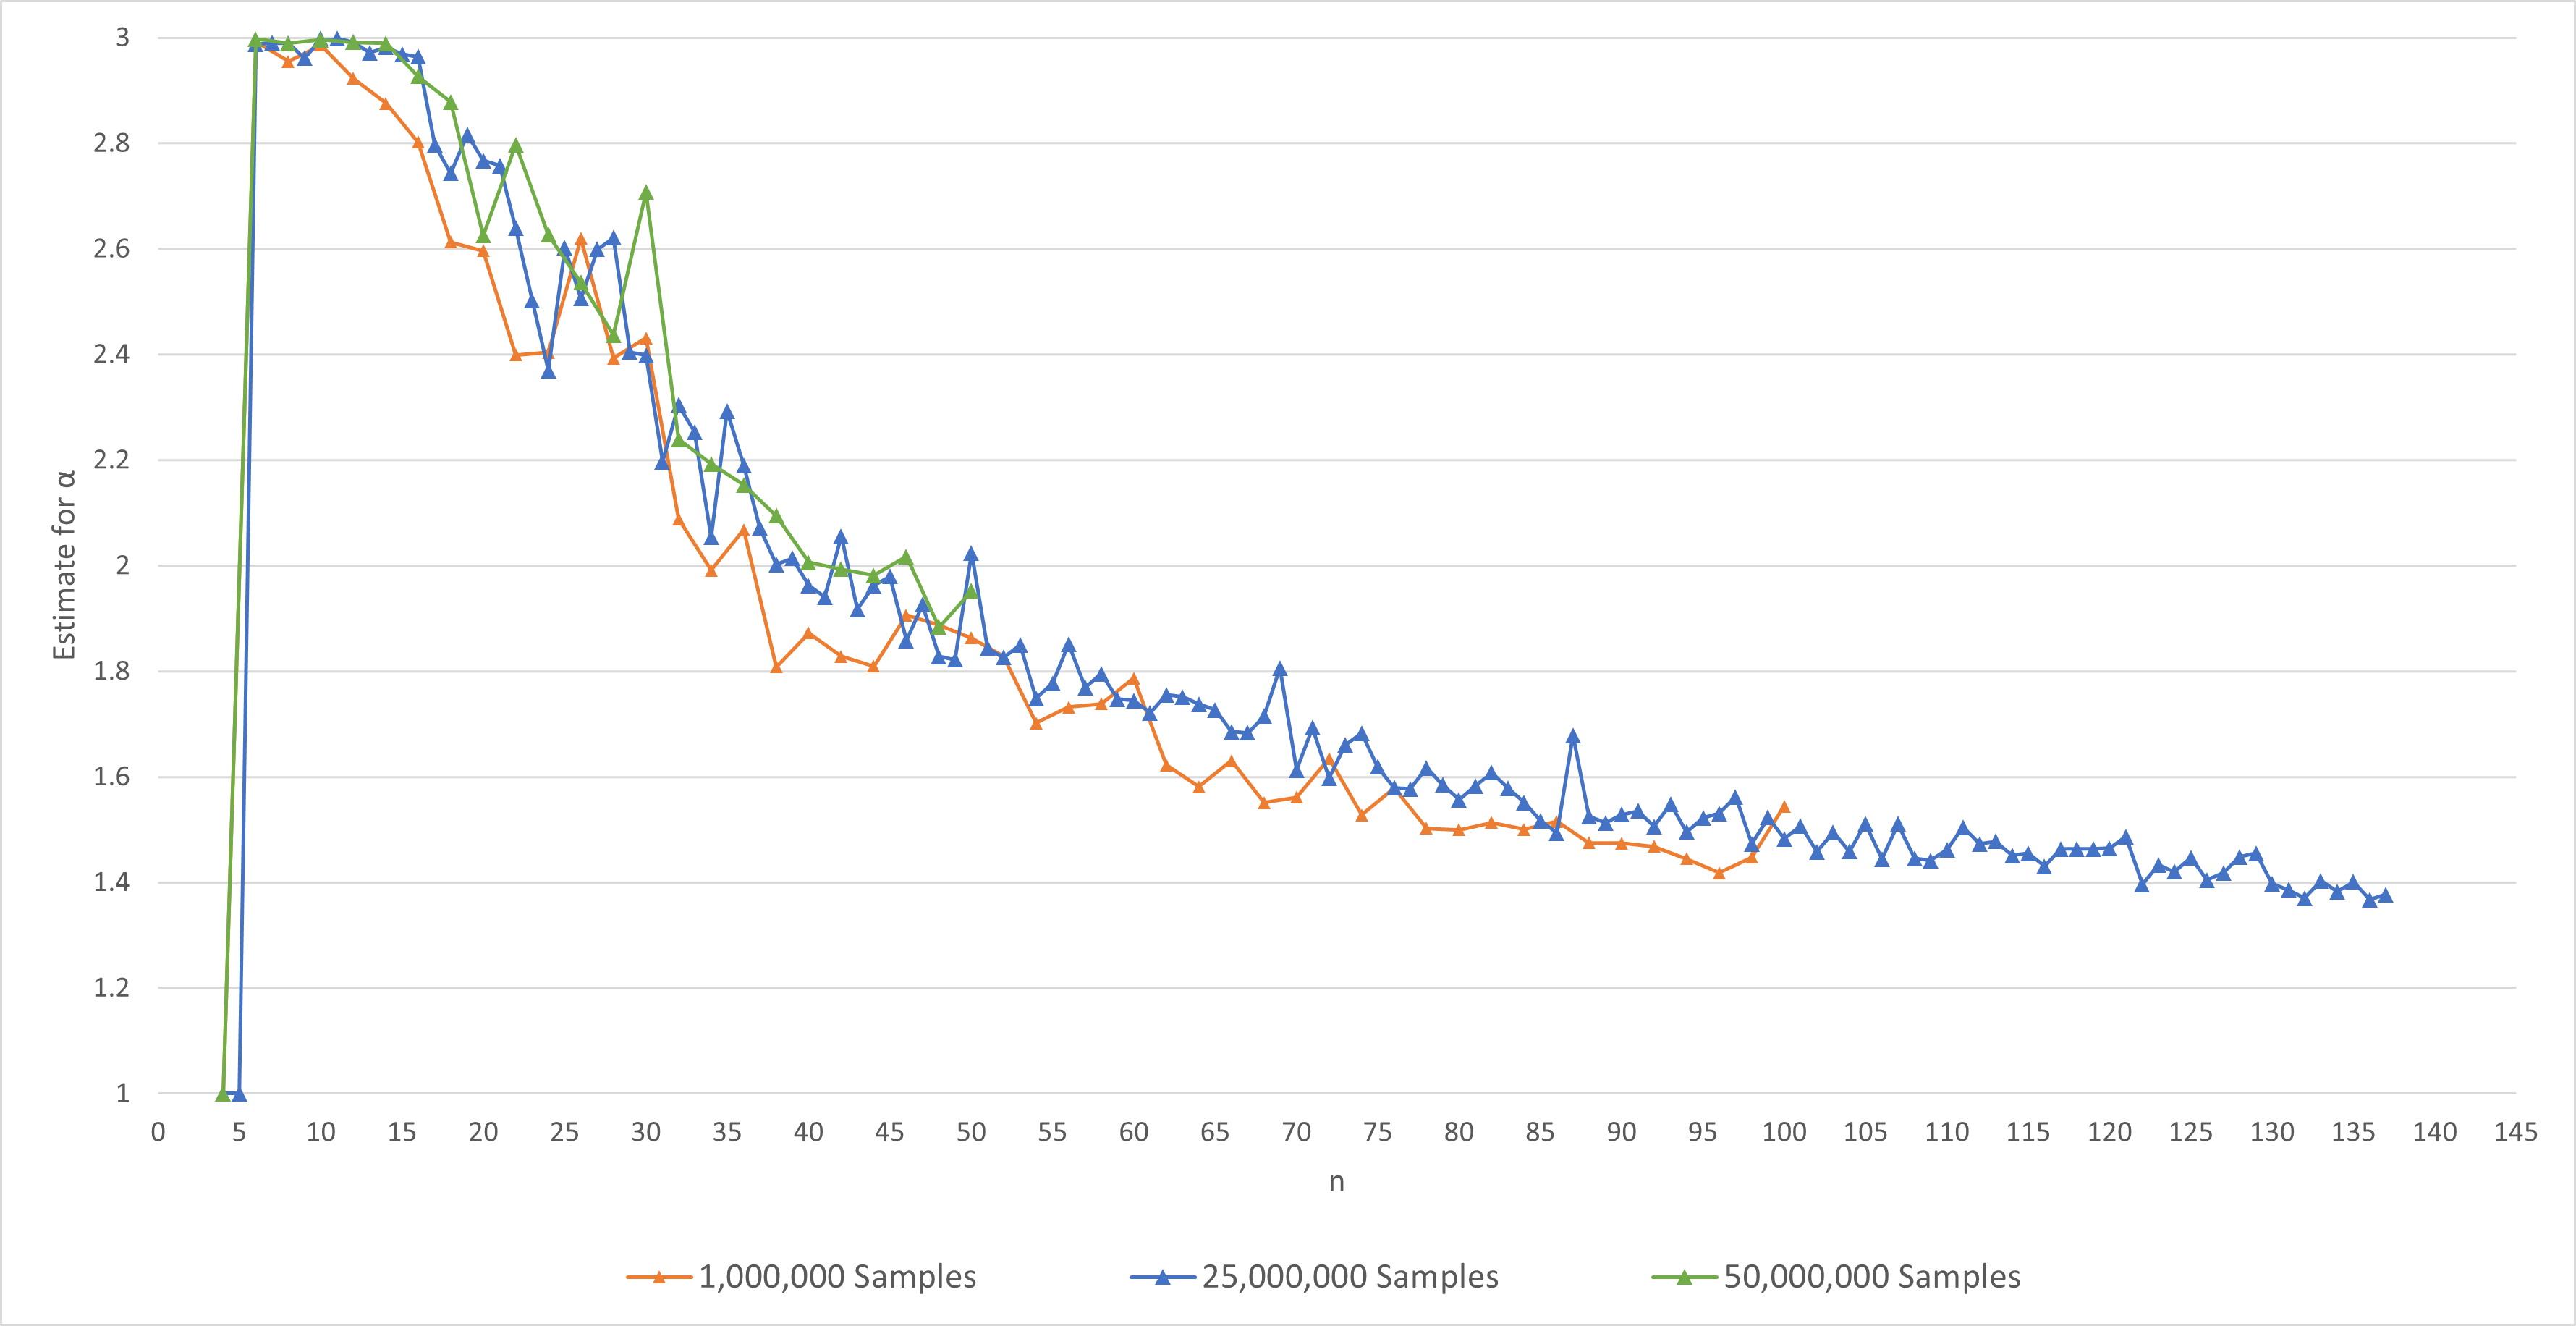
\includegraphics[scale=.55]{scatter-alpha-n-labelled.png}
\end{center}
\caption{Results of Random Sampling for $d=1$. Each data point corresponds to the result of \textcolor{RedOrange}{1} / \textcolor{MidnightBlue}{25} / \textcolor{OliveGreen}{50} million samples.}\label{res_rsample}
\end{figure}
\begin{figure}
\begin{center}
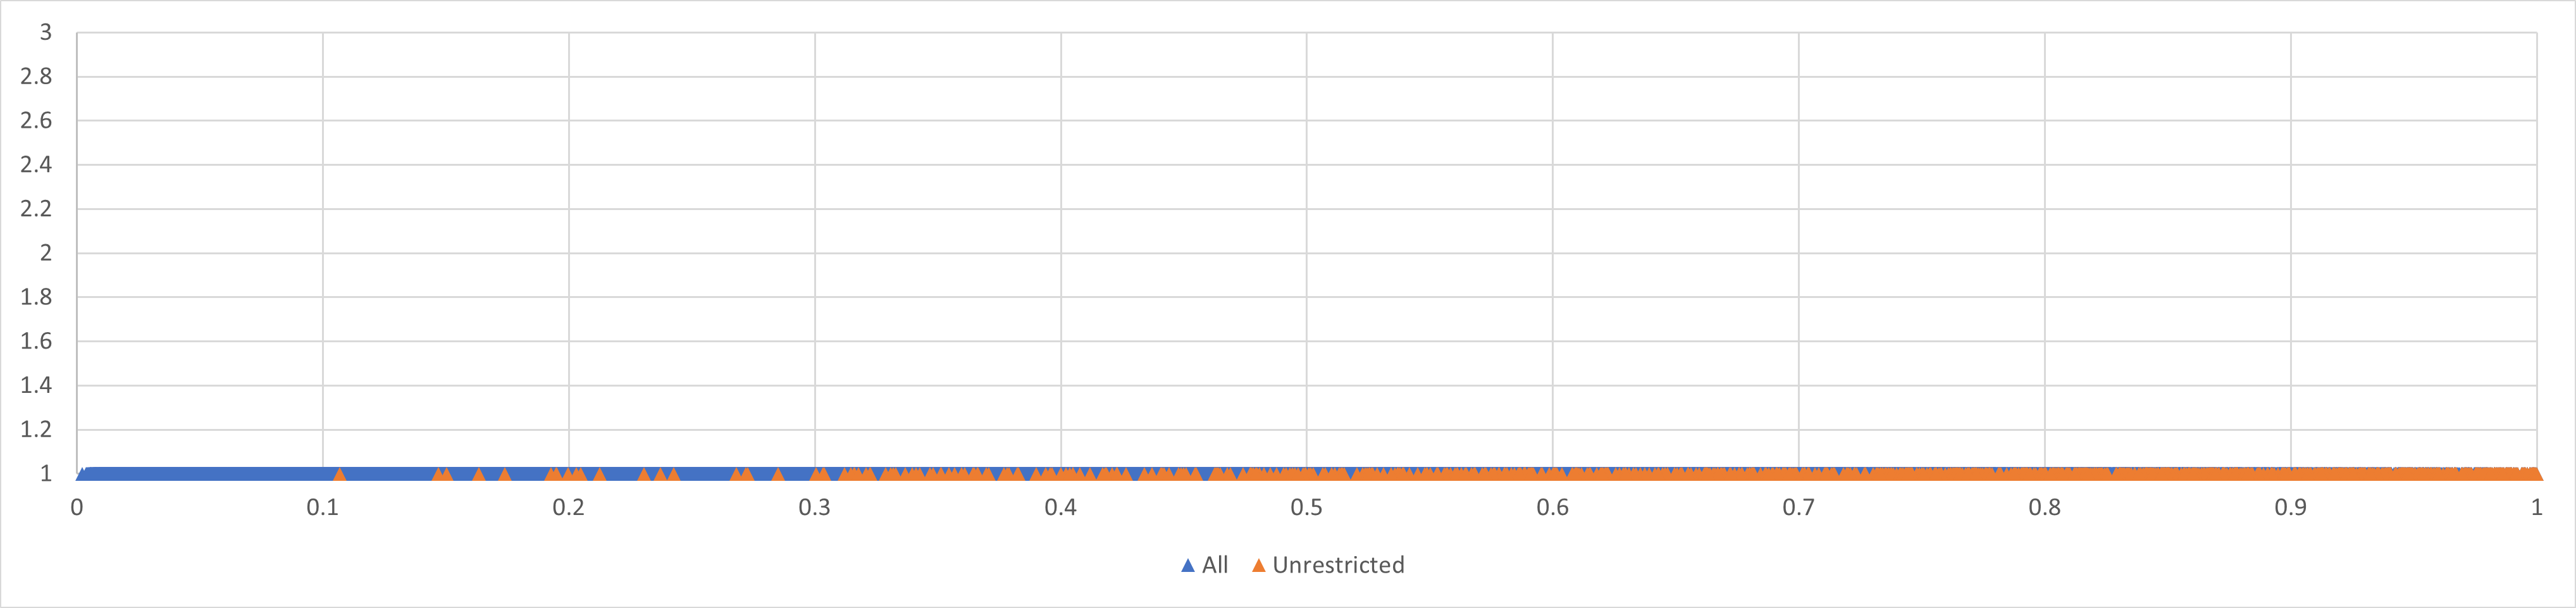
\includegraphics[scale=.48]{scatter-alpha-4-50-1000.png}
\end{center}
\caption{Results of Random Sampling for $d=1$ and $n=4$ with $50\cdot 1000$ samples. Each data point corresponds to the result of $\frac{\text{opt}(b)}{\Vert Rb\Vert_\infty}$ for one sampled $b$. The results of the unrestrictedly generated samples with $\varsigma=1$ are marked.}\label{res_rsample_4}
\end{figure}
\begin{figure}
\begin{center}
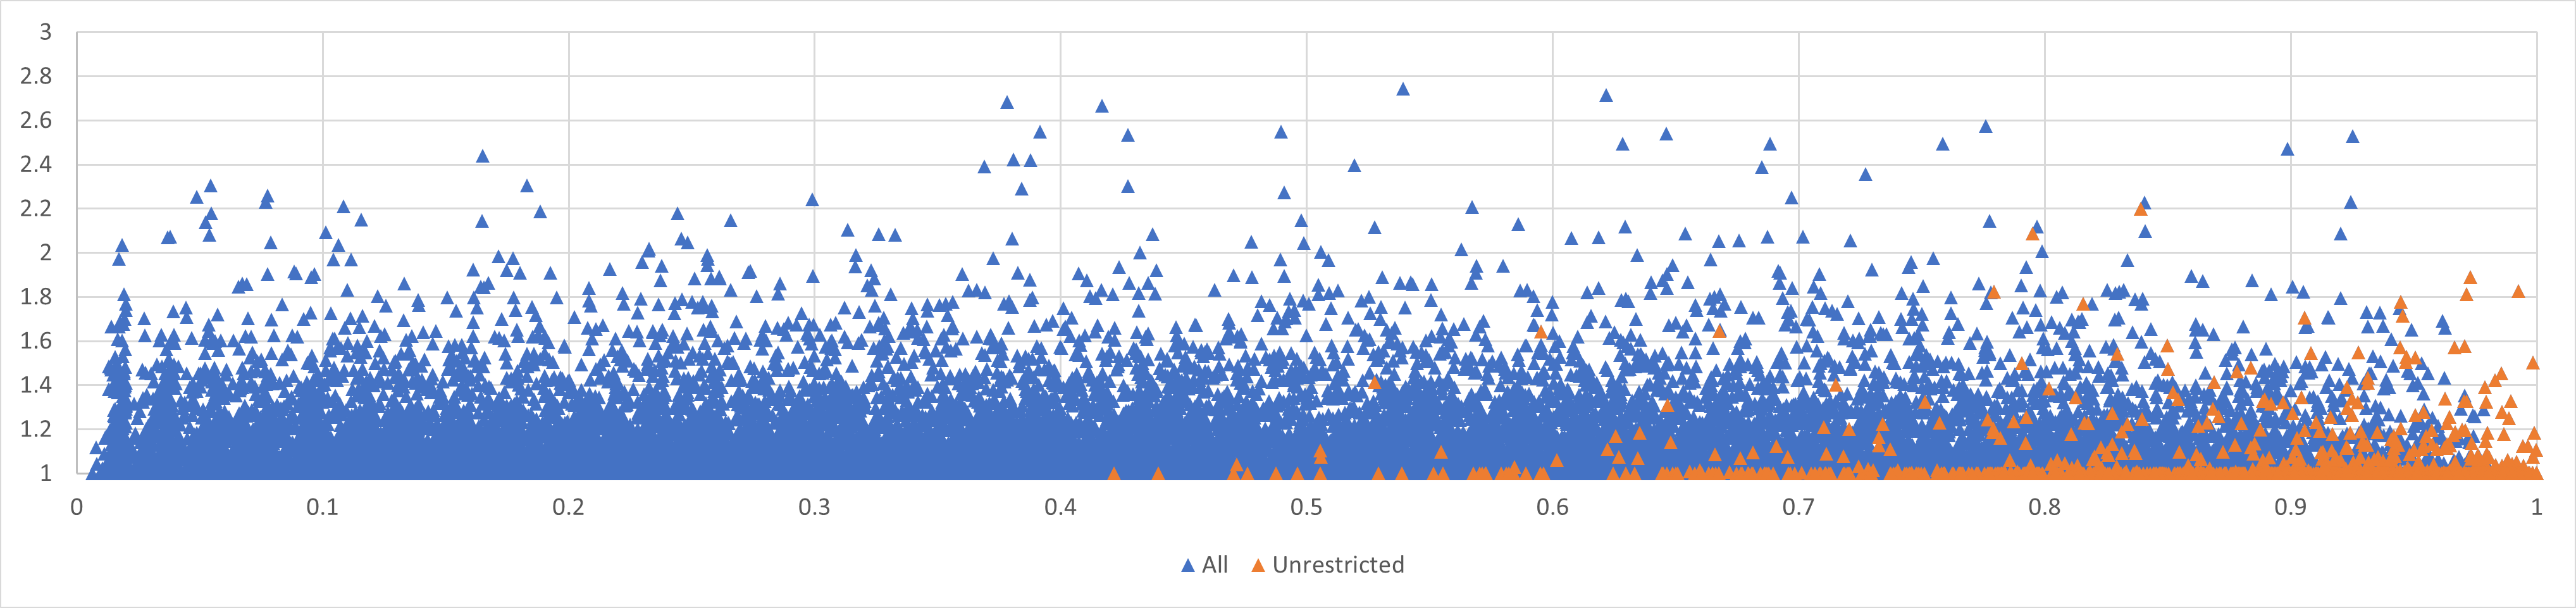
\includegraphics[scale=.48]{scatter-alpha-8-50-1000.png}
\end{center}
\caption{Results of Random Sampling for $d=1$ and $n=8$ with $50\cdot 1000$ samples. Each data point corresponds to the result of $\frac{\text{opt}(b)}{\Vert Rb\Vert_\infty}$ for one sampled $b$. The results of the unrestrictedly generated samples with $\varsigma=1$ are marked.}\label{res_rsample_8}
\end{figure}
\begin{figure}
\begin{center}
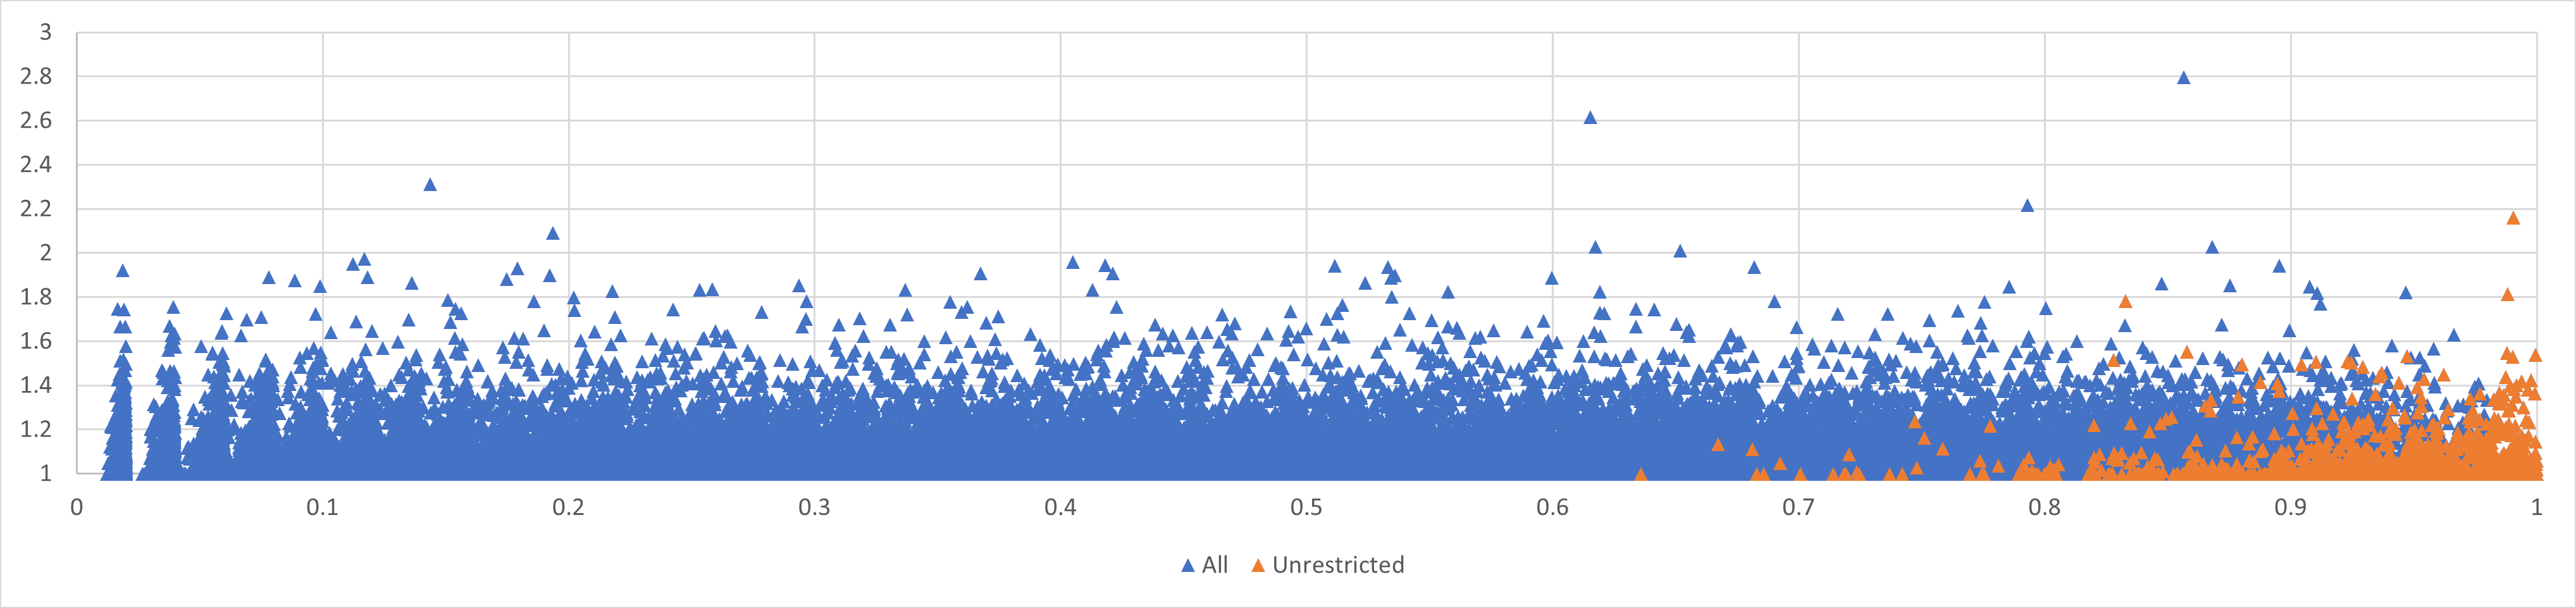
\includegraphics[scale=.48]{scatter-alpha-16-50-1000.png}
\end{center}
\caption{Results of Random Sampling for $d=1$ and $n=16$ with $50\cdot 1000$ samples. Each data point corresponds to the result of $\frac{\text{opt}(b)}{\Vert Rb\Vert_\infty}$ for one sampled $b$. The results of the unrestrictedly generated samples with $\varsigma=1$ are marked.}\label{res_rsample_16}
\end{figure}
\begin{figure}
\begin{center}
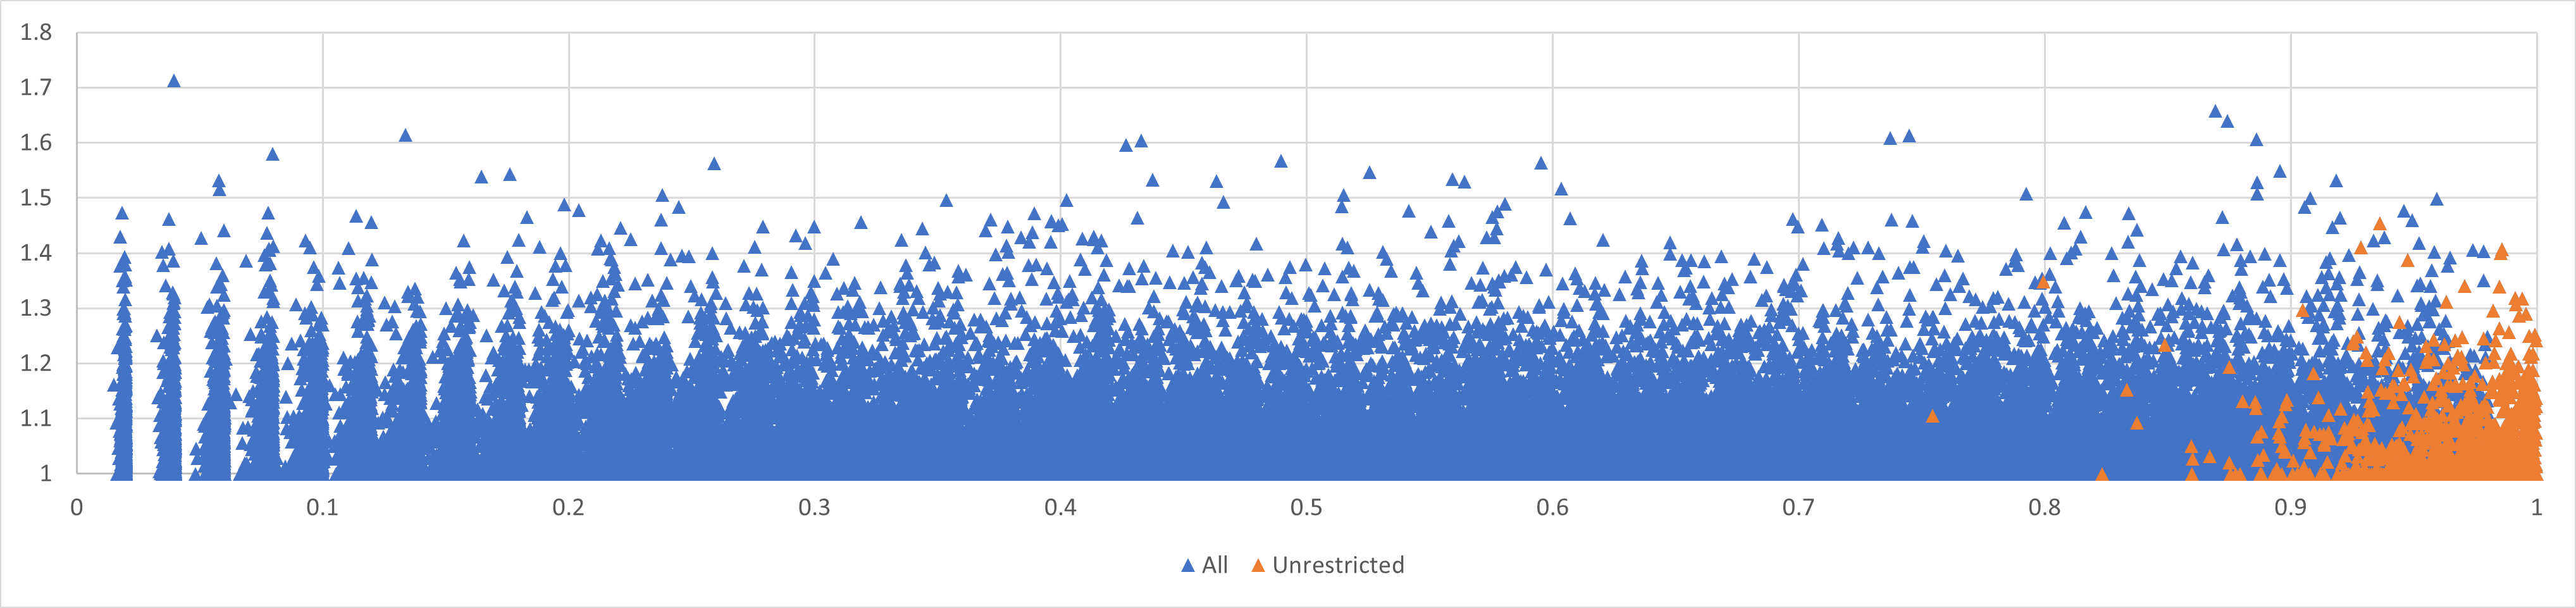
\includegraphics[scale=.48]{scatter-alpha-32-50-1000.png}
\end{center}
\caption{Results of Random Sampling for $d=1$ and $n=32$ with $50\cdot 1000$ samples. Each data point corresponds to the result of $\frac{\text{opt}(b)}{\Vert Rb\Vert_\infty}$ for one sampled $b$. The results of the unrestrictedly generated samples with $\varsigma=1$ are marked.}\label{res_rsample_32}
\end{figure}
\begin{figure}
\begin{center}
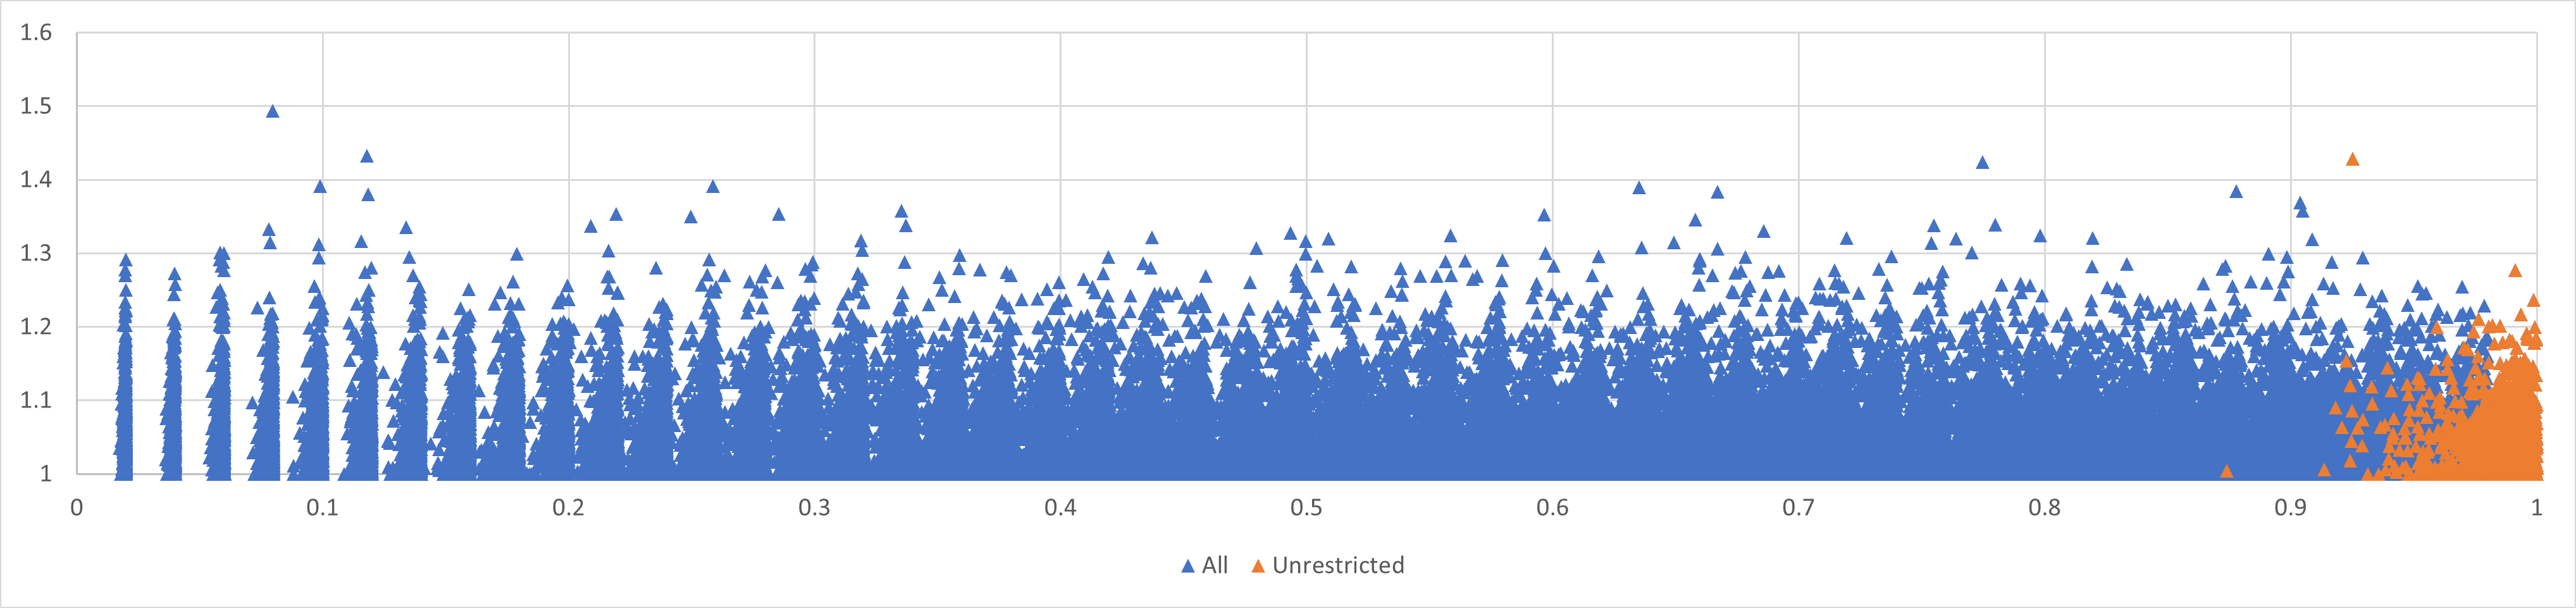
\includegraphics[scale=.48]{scatter-alpha-64-50-1000.png}
\end{center}
\caption{Results of Random Sampling for $d=1$ and $n=64$ with $50\cdot 1000$ samples. Each data point corresponds to the result of $\frac{\text{opt}(b)}{\Vert Rb\Vert_\infty}$ for one sampled $b$. The results of the unrestrictedly generated samples with $\varsigma=1$ are marked.}\label{res_rsample_64}
\end{figure}
Taking a look at the evaluations of $\alpha$, we can conclude that $\alpha=3$ can be used for our approximator at $d=1$. Values nearly at $3$, like $2.99758364093494$, were reached in most samplings for small $n$, but no estimate was found that would suggest $\alpha<1$ or $\alpha>3$. (Note that due to numerical errors, sometimes the estimate is $0.99999999...$ instead of $1$.)\\
For bigger $n$ at $d=1$, the estimates of $\alpha$ decreased overall. Since an increase in samples results in higher estimates, but only slightly increasing relative to the number of samples, it might be necessary to choose another strategy for sampling in order to get better estimates in acceptable time.\\

It seems that $\alpha=3$ should be a good choice for $\alpha$, but since the approximator will have even better congestion approximations for \emph{most} demands, it can be chosen even smaller. This evaluation suggests choosing $\alpha=3$ as parameter when looking for a correct $\alpha$, or $\alpha\approx 2\pm 0.5$ as value leading to less iterations on average.

\chapter{Final Remarks}
There are many possible improvements that lie at hand, but that were omitted in this thesis due to temporal reasons. Those include the enhancements and alternatives discussed for the golden section search, some steps of proofs that could be shown in more detail, a comparison with Nesterov's accelerated gradient descent method instead of the naive steepest descent at the step size optimization, more samplings for $\alpha$ (for example, the suggestions from the implementation chapter, namely randomized cut with maximum congestion or a pre-calculation of the approximate optimal flow value) and optimizations of the data structures.\\
Also, \texttt{AlmostRoute} could be extended to also return the potential threshold cuts, and an evaluation of \texttt{CompleteRoute} can be done.\\
The repository is public - if desired, feel free to contact me: \url{js97.sw@gmail.com}.\\
I finally want to thank Prof. Dr. Harald Räcke for supervising and advising this thesis with interesting ideas, helpful inputs and all the time to answer my many questions, and Jonah Sherman for his great publication.

%\clearpage
%
\listoffigures % Abbildungsverzeichnis
\printglossary[type=\acronymtype,title=Abkürzungsverzeichnis] % Abkürzungsverzeichnis

%\listoftables % Tabellenverzeichnis

\onehalfspacing

%\addchap{Tabellenvarianten}


\printbibliography
\end{document}
